


%% PhysicsOlympiad 1994 Screening Exam
%%----------------------------------------
\element{aapt}{
\begin{question}{olympiad-1994-q01}
    A motorist travels \SI{320}{\kilo\meter} at \SI{80}{\kilo\meter\per\hour} and then \SI{320}{\kilo\meter} at \SI{100}{\kilo\meter\per\hour}.
    What is the average speed of the motorist for the entire trip?
    \begin{multicols}{3}
    \begin{choices}
        \wrongchoice{\SI{84}{\kilo\meter\per\hour}}
      \correctchoice{\SI{89}{\kilo\meter\per\hour}}
        \wrongchoice{\SI{90}{\kilo\meter\per\hour}}
        \wrongchoice{\SI{91}{\kilo\meter\per\hour}}
        \wrongchoice{\SI{95}{\kilo\meter\per\hour}}
    \end{choices}
    \end{multicols}
\end{question}
}

\element{aapt}{
\begin{question}{olympiad-1994-q02}
    A sports car is stopped at a light.
    At $t=0$ the light changes and the sports car accelerates at a constant \SI{2.0}{\meter\per\second\squared}.
    At $t=\SI[fraction-function=\tfrac]{10/3}{\second}$ a station wagon traveling at a constant \SI{15}{\meter\per\second} in the same direction passes the stop light.
    When does the station wagon catch up to the sports car?
    \begin{multicols}{3}
    \begin{choices}
        \wrongchoice{never}
      \correctchoice{$t = \SI{5.0}{\second}$}
        \wrongchoice{$t = \SI{7.5}{\second}$}
        \wrongchoice{$t = \SI{12}{\second}$}
        \wrongchoice{$t = \SI{21}{\second}$}
    \end{choices}
    \end{multicols}
\end{question}
}

\element{aapt}{
\begin{question}{olympiad-1994-q03}
    A ball is thrown from ground level with an initial velocity of $v_0$ in the upward direction.
    It reaches a maximum height $y$ and returns to ground level at time $t$ after it was thrown.
    If its initial velocity is doubled,
        it will be in the air for time \rule[-0.1pt]{4em}{0.1pt} and reach a maximum height \rule[-0.1pt]{4em}{0.1pt}.
    \begin{multicols}{3}
    \begin{choices}
        \wrongchoice{$t$; $4y$}
        \wrongchoice{$2t$; $y$}
        \wrongchoice{$2t$; $2y$}
      \correctchoice{$2t$; $4y$}
        \wrongchoice{$4t$; $2y$}
    \end{choices}
    \end{multicols}
\end{question}
}

\element{aapt}{
\begin{question}{olympiad-1994-q04}
    %% modified to make self contained
    A ball is thrown from ground level with an initial velocity of $v_0$ in the upward direction.
    It reaches a maximum height $y$ and returns to ground level at time $t$ after it was thrown.
    %% start question
    The ball is then taken to mars where the acceleration due to gravity is approximately \SI{4}{\meter\per\second\squared} ($0.4 g_E$).
    It is thrown from ground level with the same initial velocity as it originally had on Earth,
        $v_0$ in the upward direction.
    On Mars,
        it will be in the air for time \rule[-0.1pt]{4em}{0.1pt} and reach a maximum height \rule[-0.1pt]{4em}{0.1pt}.
    \begin{multicols}{3}
    \begin{choices}
        \wrongchoice{$0.5 t$; $2.5 y$}
        \wrongchoice{$0.4 t$; $6.25 y$}
      \correctchoice{$2.5 t$; $2.5 y$}
        \wrongchoice{$6.25 t$; $2.5 y$}
        \wrongchoice{$6.25 t$; $6.25 y$}
    \end{choices}
    \end{multicols}
\end{question}
}

\element{aapt}{
\begin{question}{olympiad-1994-q05}
    A top is spinning in the direction shown in the accompanying figure.
    \begin{center}
    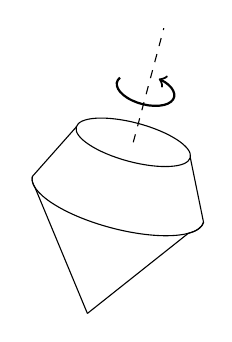
\begin{tikzpicture}
    \begin{scope}[rotate=-15,scale=0.75]
        %% top
        \draw (0,0) circle (1cm and 0.33cm);
        \draw (-1.5,-1) arc(180:360:1.5cm and 0.495cm);
        %\draw (0,-3) -- ++(130:2.0);
        \draw (-1,0) -- (-1.5,-1) arc(180:200:1.5cm and 0.495cm) -- (0,-3);
        \draw (+1,0) -- (+1.5,-1) arc(360:330:1.5cm and 0.495cm) -- (0,-3);
        %% spinning
        \draw[thick,->] (-0.5,1) arc (-200:70:0.5cm and 0.25cm);
        %% Axis
        \draw[dashed] (0,0) -- (0,2);
    \end{scope}
    \end{tikzpicture}
    \end{center}
    Its axis of rotation makes an angle of \ang{15} with the vertical.
    Assume friction can be neglected.
    The magnitude of the top's angular momentum will \rule[-0.1pt]{4em}{0.1pt} while its direction will \rule[-0.1pt]{4em}{0.1pt}.
    \begin{choices}
        \wrongchoice{increase; precess in the counterclockwise direction when seen from above.}
        \wrongchoice{increase; not precess}
        \wrongchoice{remain the same; not precess}
        \wrongchoice{remain the same; precess in the clockwise direction when seen from above.}
      \correctchoice{remain the same; precess in the counterclockwise direction when seen from above.}
    \end{choices}
\end{question}
}

\element{aapt}{
\begin{question}{olympiad-1994-q06}
    Three air track cars,
        shown in the accompanying figure,
        all have the same mass $m$.
    Cars 2 and 3 are initially at rest.
    Car 1 is moving to the right with speed $v$.
    \begin{center}
    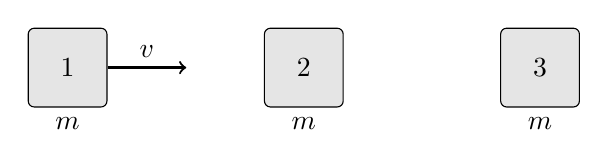
\begin{tikzpicture}
        %% Blocks
        \node[draw,minimum size=1cm,rounded corners=0.5ex,fill=white!90!black] (A) at (-3,0) {1};
        \node[draw,minimum size=1cm,rounded corners=0.5ex,fill=white!90!black] (B) at (+0,0) {2};
        \node[draw,minimum size=1cm,rounded corners=0.5ex,fill=white!90!black] (C) at (+3,0) {3};
        %% masses ??
        \node[anchor=north] at (A.south) {$m$};
        \node[anchor=north] at (B.south) {$m$};
        \node[anchor=north] at (C.south) {$m$};
        %% Arrows
        \draw[thick,->] (A.east) -- ++(0:1cm) node[pos=0.5,anchor=south] {$v$};
    \end{tikzpicture}
    \end{center}
    Car 1 collides with car 2 and sticks to it.
    The 1-2 combination collides elastically with car 3.
    Which of the following is most nearly the final speed of the 1-2 combination?
    \begin{multicols}{3}
    \begin{choices}
      \correctchoice{$0.17 v$}
        \wrongchoice{$0.50 v$}
        \wrongchoice{$0.67 v$}
        \wrongchoice{$0.80 v$}
        \wrongchoice{$1.0 v$}
    \end{choices}
    \end{multicols}
\end{question}
}

\element{aapt}{
\begin{question}{olympiad-1994-q07}
    A cube with mass $M$ starts at rest at point 1 at a height $4R$,
        where $R$ is the radius of the circular part of the track.
    The cube slides down the frictionless track and around the loop.
    \begin{center}
    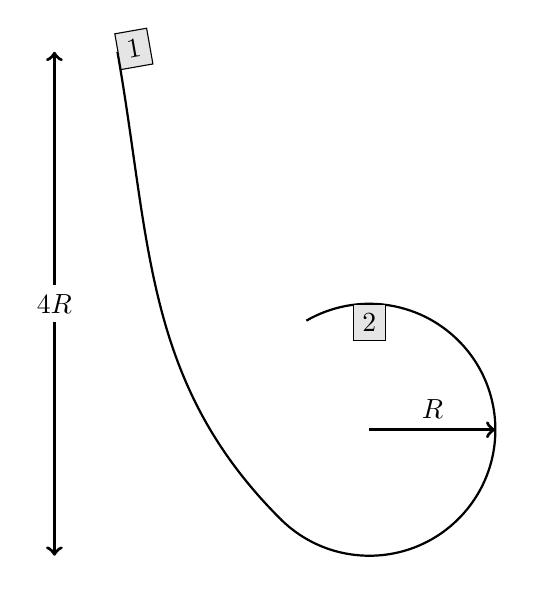
\begin{tikzpicture}[scale=0.8]
        %% Track
        \draw[thick] (-4,6) to[out=280,in=135] (225:2);
        \draw[thick] (225:2) arc(-135:120:2);
        \draw[very thick,->] (0,0) -- (2,0) node[pos=0.5,anchor=south] {$R$};
        %% block 1
        \node[draw,fill=white!90!black,minimum size=0.25,anchor=west,rotate=10] at (-4,6) {$1$};
        %% block 2
        \node[draw,fill=white!90!black,minimum size=0.25,anchor=north] at (90:2) {$2$};
        %% 6R
        \draw[very thick,<->] (-5,-2) -- (-5,6) node[pos=0.5,anchor=center,fill=white] {$4R$};
    \end{tikzpicture}
    \end{center}
    The force that the track exerts on the cube at point 2 is most nearly \rule[-0.1pt]{4em}{0.1pt} times the cube's weight $Mg$.
    \begin{multicols}{3}
    \begin{choices}
        \wrongchoice{1}
        \wrongchoice{2}
      \correctchoice{3}
        \wrongchoice{4}
        \wrongchoice{5}
    \end{choices}
    \end{multicols}
\end{question}
}

\element{aapt}{
\begin{question}{olympiad-1994-q08}
    An astronaut with weight $W$ on Earth lands on a planet with mass 0.1 times the mass of Earth and radius 0.5 times the radius of Earth.
    The astronaut's weight is \rule[-0.1pt]{4em}{0.1pt} on the planet.
    \begin{multicols}{3}
    \begin{choices}
        \wrongchoice{$0.02 W$}
        \wrongchoice{$0.04 W$}
        \wrongchoice{$0.2 W$}
      \correctchoice{$0.4 W$}
        \wrongchoice{$ W$}
    \end{choices}
    \end{multicols}
\end{question}
}

\element{aapt}{
\begin{question}{olympiad-1994-q09}
    A horizontal force $F$, represented by the arrow in the figure below,
        is used to push a block of weight $mg$ up an inclined plane making an angle of $\theta$ with the horizontal.
    The coefficient of friction between the plane and the block is $\mu$.
    \begin{center}
    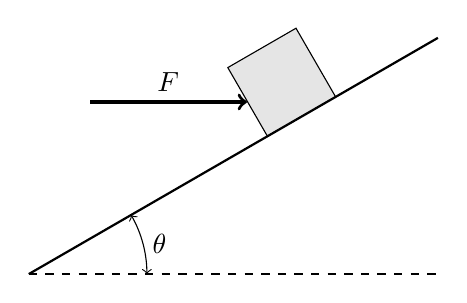
\begin{tikzpicture}
        %% incline
        \draw[thick] (0,0) -- (30:6);
        \draw[thick,dashed] (0,0) -- (0:5.196);
        \draw[<->] (1.5,0) arc (0:30:1.5) node[pos=0.5,anchor=west] {$\theta$};
        %% block
        \node[draw,anchor=south,minimum size=1cm,rotate=30,fill=white!90!black] (A) at (30:4) {};
        %% force
        \draw[very thick,<-] (A.west) -- ++(180:2) node[pos=0.5,anchor=south] {$F$};
    \end{tikzpicture}
    \end{center}
    The magnitude of the frictional force acting on the block is:
    \begin{multicols}{2}
    \begin{choices}
        \wrongchoice{$\mu mg\cos\theta$}
        \wrongchoice{$\dfrac{\mu mg}{\cos\theta}$}
      \correctchoice{$\mu\left( mg \cos\theta + F\sin\theta\right)$}
        \wrongchoice{$\mu\left(F\cos\theta - mg\sin\theta\right)$}
        \wrongchoice{$\mu F\cos\theta$}
    \end{choices}
    \end{multicols}
\end{question}
}

\element{aapt}{
\begin{question}{olympiad-1994-q10}
    A child of mass $M$ stands on the edge of a merry-go-round of radius $R$ and moment of inertia $I$.
    Both the merry-go-round and child are initially at rest.
    The child walks around the circumference with speed $v$ with respect to the ground.
    What is the magnitude of the angular velocity of the merry-go-round with respect to the ground?
    \begin{multicols}{2}
    \begin{choices}
      \correctchoice{zero}
        \wrongchoice{$\omega = \dfrac{MRv}{I}$}
        \wrongchoice{$\omega = \dfrac{v}{R}$}
        \wrongchoice{$\omega = \dfrac{MRv}{I-MR^2}$}
        \wrongchoice{$\omega = \dfrac{MRv}{I+MR^2}$}
    \end{choices}
    \end{multicols}
\end{question}
}

\element{aapt}{
\begin{question}{olympiad-1994-q11}
    A rigid rod of mass $M$ and length $L$ has moment of inertia $\frac{1}{12} ML^2$ about its center of mass.
    A sphere of mass $m$ and radius $R$ has moment of inertia $\frac{2}{5} MR^2$ about its center of mass.
    A combined system is formed by centering the sphere at one end of the rod and placing an axis at the other (see accompanying figure).
    \begin{center}
    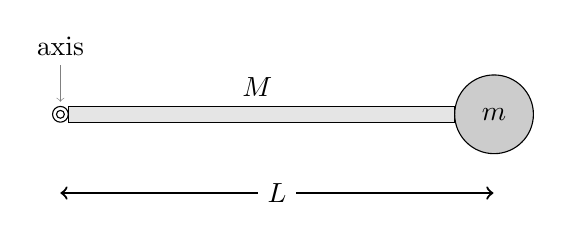
\begin{tikzpicture}
        %% Pivot Point
        \draw (0,0) circle (0.05cm);
        \draw (0,0) circle (0.1cm);
        \node[pin={[pin distance=5mm,pin edge={<-,shorten <=1pt}]90:axis}] at (0,0) {};
        %% Rod
        \draw[fill=white!90!black] (0.1,0.1) rectangle (5,-0.1);
        \node[anchor=south] at (2.5,0.1) {$M$};
        \draw[thick,<->] (0,-1) -- (5.5,-1) node[pos=0.5,anchor=center,fill=white] {$L$};
        %% Ball
        \node[draw,fill=white!80!black,circle,anchor=west,minimum size=1cm] at (5,0) {$m$};
    \end{tikzpicture}
    \end{center}
    What is the moment of inertia of the combined system about the axis shown?
    \begin{choices}
        \wrongchoice{$I = \dfrac{1}{12} ML^2 + \dfrac{2}{5} MR^2$}
        \wrongchoice{$I = \dfrac{1}{12} ML^2 + \dfrac{2}{5} MR^2 + mL^2$}
      \correctchoice{$I = \dfrac{1}{3} ML^2 + \dfrac{2}{5} MR^2 + mL^2$}
        \wrongchoice{$I = \dfrac{1}{12} ML^2 + mL^2$}
        \wrongchoice{$I = \dfrac{1}{3} ML^2 + mL^2$}
    \end{choices}
\end{question}
}

\element{aapt}{
\begin{question}{olympiad-1994-q12}
    A rocket is launched from the surface of a planet with mass $M$ and radius $R$.
    What is the minimum velocity the rocket must be given to completely escape from the planet's gravitational field?
    \begin{multicols}{2}
    \begin{choices}
        \wrongchoice{$v = \sqrt{\dfrac{2GM}{R^2}}$}
      \correctchoice{$v = \sqrt{\dfrac{2GM}{R}}$}
        \wrongchoice{$v = \sqrt{\dfrac{GM}{R^2}}$}
        \wrongchoice{$v = \sqrt{\dfrac{GM}{R}}$}
        \wrongchoice{$v = \sqrt{GM}$}
    \end{choices}
    \end{multicols}
\end{question}
}

\element{aapt}{
\begin{question}{olympiad-1994-q13}
    A uniform rod of length $L$ and weight $W_R$ is suspended as shown in the accompanying figure.
    \begin{center}
    \begin{tikzpicture}
        %% and wall
        \draw[thick] (0,-1) -- (0,6);
        \node[anchor=east,fill,pattern=north east lines,minimum width=0.1cm, minimum height=7cm] at (0,2.5) {};
        %% hinge and rod
        \draw (0.1,0) circle (0.1);
        \draw[fill=white!90!black] (0.2,-0.1) rectangle (6,0.1);
        \draw[very thick,->] (6,0.1) -- (6,-2) node[anchor=south east] {$W$};
        %% Cable
        \draw (6,0.1) -- (0,5);
        \draw[very thick,->] (6,0.1) -- ++(140.76:2) node[anchor=south west] {$T$};
    \end{tikzpicture}
    \end{center}
    A weight $W$ is added to the end of the rod.
    The support wire is at an angle $\theta$ to the rod.
    What is the tension $T$ in the wire?
    \begin{multicols}{2}
    \begin{choices}
        \wrongchoice{$T = \dfrac{W}{\sin\theta}$}
        \wrongchoice{$T = W + W_R$}
        \wrongchoice{$T = W + \dfrac{1}{2}W_R$}
      \correctchoice{$T = \dfrac{W + \dfrac{1}{2}W_R}{\sin\theta}$}
        \wrongchoice{$T = \dfrac{W + W_R}{\sin\theta}$}
    \end{choices}
    \end{multicols}
\end{question}
}

\element{aapt}{
\begin{question}{olympiad-1994-q14}
    A hollow vertical cylinder of radius $R$ is rotated with angular velocity $\omega$ about an axis through its center.
    \begin{center}
    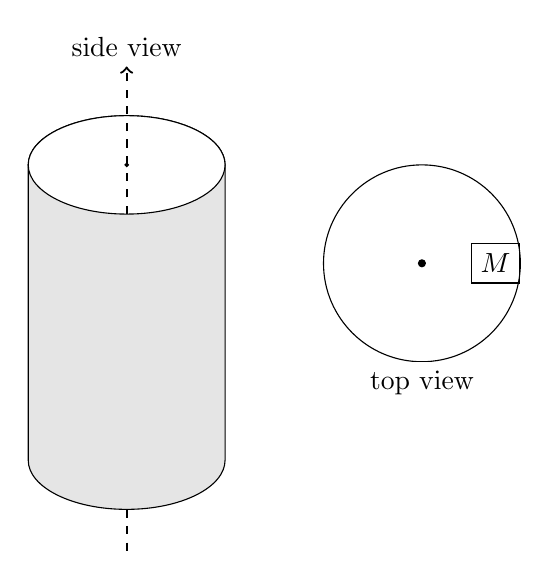
\begin{tikzpicture}[scale=1.25]
        \begin{scope}[xshift=-1.5cm]
            \draw[fill=white!90!black] (-1,0) arc (180:0:1cm and 0.5cm) -- (1,-3) arc(0:-180:1cm and 0.5cm) -- (-1,0) --cycle;
            %\draw[fill=white!50!black] (-1,0) arc(180:-180:1cm and 0.5cm);
            \draw[fill=white] (-1,0) arc(180:-180:1cm and 0.5cm);
            \draw[fill] (0,0) circle (0.5pt);
            \draw[thick,dashed] (0,-3.5) -- (0,-4);
            \draw[thick,dashed,->] (0,-0.5) -- (0,1) node[anchor=south,text width=5em,text centered] {side view};
        \end{scope}
        \begin{scope}[xshift=+1.5cm,yshift=-1cm]
            %\draw[fill=white!50!black] (0,0) circle (1cm);
            \draw[fill=white] (0,0) circle (1cm);
            \draw[fill] (0,0) circle (1pt);
            \node[anchor=north,fill=white] at (0,-1) {top view};
            \node[draw,minimum size=0.5cm,anchor=east] at (1,0) {$M$};
        \end{scope}
    \end{tikzpicture}
    \end{center}
    What is the minimum coefficient of static friction necessary to keep the mass $M$ suspended on the inside of the cylinder as it rotates?
    \begin{multicols}{2}
    \begin{choices}
        \wrongchoice{$\mu = \dfrac{gR}{\omega^2}$}
        \wrongchoice{$\mu = \dfrac{\omega^2 g}{R}$}
        \wrongchoice{$\mu = \dfrac{\omega^2 R}{g}$}
        \wrongchoice{$\mu = \dfrac{\omega^2}{gR}$}
      \correctchoice{$\mu = \dfrac{g}{\omega^2 R}$}
    \end{choices}
    \end{multicols}
\end{question}
}

\element{aapt}{
\begin{question}{olympiad-1994-q15}
    A block of mass $M$ is attached to a relaxed spring with force constant $k$,
        placed on a frictionless inclined plane as shown in the accompanying figure, and released.
    \begin{center}
    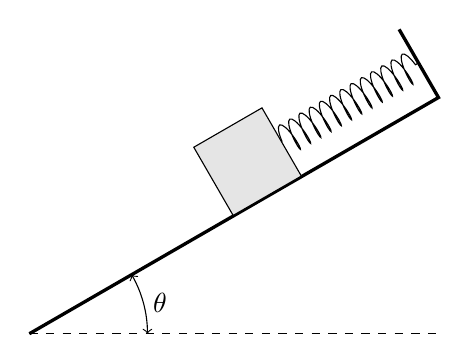
\begin{tikzpicture}
        %% incline
        \draw[very thick] (0,0) -- (30:6) --++(120:1);
        \draw[dashed] (0,0) -- (0:5.20);
        \draw[<->] (1.5,0) arc (0:30:1.5) node[pos=0.5,anchor=west] {$\theta$};
        %% block
        \node[draw,anchor=south east,minimum size=1cm,rotate=30,fill=white!90!black] (A) at (30:4) {};
        %% Spring
        \draw[decoration={aspect=0.2,segment length=1.5mm,amplitude=2mm,coil},decorate] (A.east) -- ++(30:2);
    \end{tikzpicture}
    \end{center}
    What is the maximum extension of the spring?
    \begin{multicols}{2}
    \begin{choices}
      \correctchoice{$x = \dfrac{2Mg\sin\theta}{k}$}
        \wrongchoice{$x = \dfrac{Mg\sin\theta}{k}$}
        \wrongchoice{$x = \dfrac{2Mg}{k}$}
        \wrongchoice{$x = \dfrac{Mg}{k}$}
        \wrongchoice{$x = \sqrt{2gM}$}
    \end{choices}
    \end{multicols}
\end{question}
}

\element{aapt}{
\begin{question}{olympiad-1994-q16}
    A simple pendulum of length $L$ and mass $m$ is attached to a moving support.
    \begin{center}
    \begin{tikzpicture}
        %% Wall
        \node[anchor=east,fill,pattern=north east lines,minimum width=0.25cm, minimum height=4.25cm] at (0,-1.85) {};
        \draw (0,0.29) rectangle (-0.29,-4);
        %% Ceiling
        \node[anchor=south,fill,pattern=north east lines,minimum width=3cm, minimum height=0.25cm] at (1.5,0) {};
        \draw (0,0) rectangle (3,0.29);
        %% Pendulum
        \draw (1.5,0) -- ++(300:3);
        \draw[fill=white!90!black] (1.5,0) ++(300:3) circle (5pt);
        %% angle
        \draw[dashed] (1.5,0) -- ++(270:3);
        \draw[<->] (1.5,0) ++(270:1.5) arc (270:300:1.5) node[pos=0.5,anchor=north] {$\theta$};
        %% length
        \draw[latex-latex] (2.5,0) -- ++(300:3) node[pos=0.5,anchor=center,fill=white,rotate=-60] {$L$};
    \end{tikzpicture}
    \end{center}
    In order for the pendulum string to make a constant angle $\theta$ with the vertical,
        the support must be moving to the:
    \begin{choices}
        \wrongchoice{right with constant acceleration $a = g\tan\theta$.}
      \correctchoice{left with constant acceleration $a = g\tan\theta$.}
        \wrongchoice{right with constant acceleration $a = g\sin\theta$.}
        \wrongchoice{right with constant velocity $v=\sqrt{Lg\tan\theta}$}
        \wrongchoice{left with constant velocity $v=\sqrt{Lg\tan\theta}$}
    \end{choices}
\end{question}
}

\element{aapt}{
\begin{question}{olympiad-1994-q17}
    A Carnot cycle takes in \SI{1000}{\joule} of heat at a high temperature of \SI{400}{\kelvin}.
    How much heat is expelled at the cooler temperature of \SI{300}{\kelvin}?
    \begin{multicols}{3}
    \begin{choices}
        \wrongchoice{zero}
        \wrongchoice{\SI{250}{\joule}}
        \wrongchoice{\SI{500}{\joule}}
      \correctchoice{\SI{750}{\joule}}
        \wrongchoice{\SI{1000}{\joule}}
    \end{choices}
    \end{multicols}
\end{question}
}

\element{aapt}{
\begin{question}{olympiad-1994-q18}
    An ideal gas is expanded at constant pressure from initial volume $V_i$ and temperature $T_i$ to final volume $V_f$ and temperature $T_f$.
    The gas has molar heat capacity $C_P$ at constant pressure.
    The amount of work done by $n$ moles of the gas during the process can be expressed:
    \begin{multicols}{2}
    \begin{choices}
        \wrongchoice{zero}
        \wrongchoice{$nRT\ln\left(\dfrac{V_f}{V_i}\right)$}
        \wrongchoice{$C_P\left(T_f-T_i\right)$}
        \wrongchoice{$nR\left(V_f-V_i\right)$}
      \correctchoice{$nR\left(T_f-T_i\right)$}
    \end{choices}
    \end{multicols}
\end{question}
}

\element{aapt}{
\begin{question}{olympiad-1994-q19}
    The average translational kinetic energy of any ideal gas depends only on:
    \begin{choices}
      \correctchoice{the absolute (Kelvin) temperature.}
        \wrongchoice{the mass of the gas.}
        \wrongchoice{the pressure of the gas.}
        \wrongchoice{the amount of the gas.}
        \wrongchoice{whether the gas is monatomic or diatomic.}
    \end{choices}
\end{question}
}

\element{aapt}{
\begin{question}{olympiad-1994-q20}
    A soap film of thickness $t$ is surrounded by air.
    It is illuminated at near normal incidence by monochromatic light which has wavelength $\lambda$ in the film.
    \begin{center}
    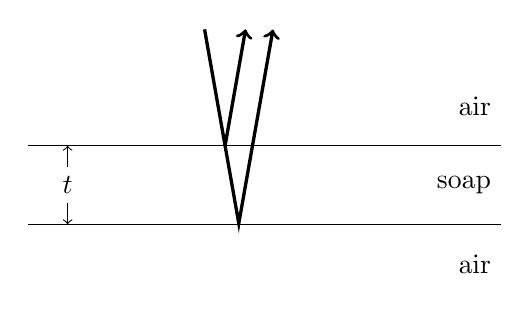
\begin{tikzpicture}
        \draw (-3,1) -- (3,1);
        \draw (-3,0) -- (3,0);
        %% thickness
        \draw[<->] (-2.5,1) -- (-2.5,0) node[pos=0.5,anchor=center,fill=white] {$t$};
        %% index of refraction
        \node[anchor=east] at (3,1.5) {air};
        \node[anchor=east] at (3,0.5) {soap};
        \node[anchor=east] at (3,-0.5) {air};
        %% Path
        \draw[very thick] (-0.5,1) -- ++(100:1.5);
        \draw[very thick,->] (-0.5,1) -- ++(80:1.5);
        \draw[very thick,->] (-0.5,1) -- ++(-80:1.003) -- ++(80:2.5);
    \end{tikzpicture}
    \end{center}
    A film thickness of \rule[-0.1pt]{4em}{0.1pt} will produce maximum brightness of the reflected light.
    \begin{multicols}{3}
    \begin{choices}
      \correctchoice{$\dfrac{\lambda}{4}$}
        \wrongchoice{$\dfrac{\lambda}{2}$}
        \wrongchoice{$\lambda$}
        \wrongchoice{$2\lambda$}
        \wrongchoice{$4\lambda$}
    \end{choices}
    \end{multicols}
\end{question}
}

\element{aapt}{
\begin{question}{olympiad-1994-q21}
    You are given two lenses,
        a converging lens with focal length \SI{+10}{\centi\meter} and a diverging lens with focal length \SI{-20}{\centi\meter}.
    Which of the following would produce a real image that is smaller than the object?
    \begin{choices}
        \wrongchoice{Placing the object \SI{5}{\centi\meter} from the converging lens.}
        \wrongchoice{Placing the object \SI{15}{\centi\meter} from the converging lens.}
      \correctchoice{Placing the object \SI{25}{\centi\meter} from the converging lens.}
        \wrongchoice{Placing the object \SI{15}{\centi\meter} from the diverging lens.}
        \wrongchoice{Placing the object \SI{25}{\centi\meter} from the diverging lens.}
    \end{choices}
\end{question}
}

\element{aapt}{
\begin{question}{olympiad-1994-q22}
    A source at rest emits waves with wavelength $\lambda$ in a medium with velocity $v$.
    \begin{center}
    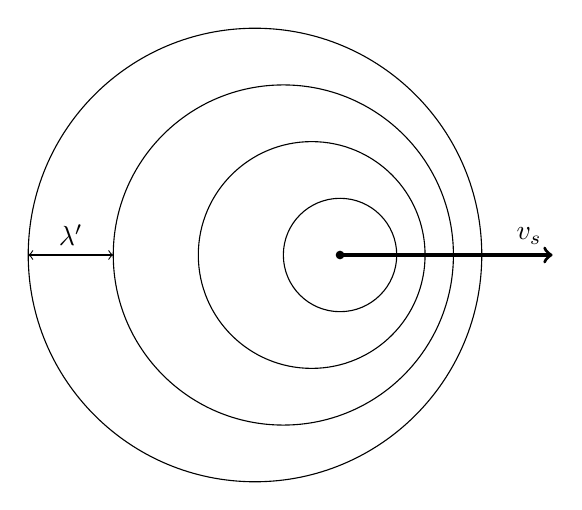
\begin{tikzpicture}[scale=0.9]
        %% Wave Fronts
        \foreach \x in {8,16,24,32} {
            \draw (-0.5 * \x mm,0) circle (\x mm);
        }
        %% Velocity
        \draw[fill] (-4mm,0) circle (1.5pt);
        \draw[very thick,->] (-4mm,0) --++(0:3) node[anchor=south east] {$v_s$};
        %% lambda prime
        \draw[<->] (-48mm,0) -- (-36mm,0) node[pos=0.5,anchor=south] {$\lambda^{\prime}$};
    \end{tikzpicture}
    \end{center}
    If the source moves to the right with velocity $v_s$,
        the distance between adjacent crests $\lambda^{\prime}$ directly behind the source is:
    \begin{multicols}{2}
    \begin{choices}
        \wrongchoice{$\dfrac{\lambda v}{v + v_s}$}
        \wrongchoice{$\dfrac{\lambda v}{v - v_s}$}
        \wrongchoice{$\lambda \left(1 + \dfrac{v}{v_s}\right)$}
      \correctchoice{$\lambda \left(1 + \dfrac{v_s}{v}\right)$}
        \wrongchoice{$\lambda \left(1 - \dfrac{v_s}{v}\right)$}
    \end{choices}
    \end{multicols}
\end{question}
}

\element{aapt}{
\begin{question}{olympiad-1994-q23}
    Two sources, in phase and a distance $d$ apart, each emit a wave of wavelength $\lambda$.
    See accompanying figure.
    \begin{center}
    \begin{tikzpicture}
        %% Two sources
        \draw[fill] (0,+1) circle (2pt);
        \draw[fill] (0,-1) circle (2pt);
        \draw[<->] (-0.3,-1) -- (-0.3,+1) node[pos=0.5,anchor=center,fill=white] {$d$};
        %% point P
        \draw[fill] (6,2) circle (1pt) node[anchor=south] {$P$};
        \draw (0,+1) -- (6,2) node[pos=0.1,anchor=south,rotate=14] {$L_2$};
        \draw (0,-1) -- (6,2) node[pos=0.1,anchor=south,rotate=37] {$L_1$};
        %% distance x
        \draw[<->] (6,0) -- (6,1.95) node[pos=0.5,anchor=center,fill=white] {$x$};
        \draw[dashed] (-0.1,0) -- (6.1,0);
    \end{tikzpicture}
    \end{center}
    Which of the choices for the path difference $\Delta L = L_1 - L_2$ will always produce constructive interference at point $P$?
    \begin{multicols}{3}
    \begin{choices}
        \wrongchoice{$d\sin\theta$}
        \wrongchoice{$\dfrac{x}{L_1}$}
        \wrongchoice{$d\left(\dfrac{x}{L_2}\right)$}
        \wrongchoice{$\dfrac{\lambda}{d}$}
      \correctchoice{$2\lambda$}
    \end{choices}
    \end{multicols}
\end{question}
}

\newcommand{\aaptOlympiadNinetyFourQTwentyFour}{
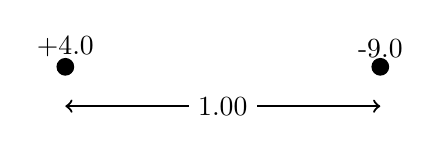
\begin{tikzpicture}
    %% charges
    \draw[fill] (-2,0) circle (3pt) node[anchor=south] {\SI{+4.0}{\micro\coulomb}};
    \draw[fill] (+2,0) circle (3pt) node[anchor=south] {\SI{-9.0}{\micro\coulomb}};
    %% length
    \draw[thick,<->] (-2,-0.5) -- (2,-0.5) node[pos=0.5,anchor=center,fill=white] {\SI{1.00}{\meter}};
\end{tikzpicture}
}

\element{aapt}{
\begin{question}{olympiad-1994-q24}
    %Refer to the following information for the next two questions.
    Two point charges of \SI{+4.00}{\micro\coulomb} and \SI{-9.00}{\micro\coulomb} are placed \SI{1.00}{\meter} apart,
        as shown in the accompanying figure.
    \begin{center}
        \aaptOlympiadNinetyFourQTwentyFour
    \end{center}
    Assume the potential goes to zero as $R$ goes to infinity.
    %% start question
    The total electric field due to the two charges is zero at a point:
    \begin{choices}
        \wrongchoice{\SI{3.00}{\meter} to the right of the \SI{-9.00}{\micro\coulomb} charge.}
        \wrongchoice{\SI{0.40}{\meter} to the right of the \SI{+4.00}{\micro\coulomb} charge.}
        \wrongchoice{\SI{0.31}{\meter} to the right of the \SI{+4.00}{\micro\coulomb} charge.}
        \wrongchoice{\SI{0.80}{\meter} to the left of the \SI{+4.00}{\micro\coulomb} charge.}
      \correctchoice{\SI{2.00}{\meter} to the left of the \SI{+4.00}{\micro\coulomb} charge.}
    \end{choices}
\end{question}
}

\element{aapt}{
\begin{question}{olympiad-1994-q25}
    %Refer to the following information for the next two questions.
    Two point charges of \SI{+4.00}{\micro\coulomb} and \SI{-9.00}{\micro\coulomb} are placed \SI{1.00}{\meter} apart,
        as shown in the accompanying figure.
    \begin{center}
        \aaptOlympiadNinetyFourQTwentyFour
    \end{center}
    Assume the potential goes to zero as $R$ goes to infinity.
    %% start question
    How much work is done moving the \SI{-9.00}{\micro\coulomb} charge from its original position to a new position \SI{2.00}{\meter} from the \SI{+4.00}{\micro\coulomb} charge?
    \begin{multicols}{3}
    \begin{choices}
        \wrongchoice{\SI{-0.324}{\joule}}
        \wrongchoice{\SI{-0.081}{\joule}}
      \correctchoice{\SI{+0.162}{\joule}}
        \wrongchoice{\SI{+0.243}{\joule}}
        \wrongchoice{\SI{+0.486}{\joule}}
    \end{choices}
    \end{multicols}
\end{question}
}

\element{aapt}{
\begin{question}{olympiad-1994-q26}
    A point charge $Q$ is placed at the center of a spherical conducting shell,
        the shaded part of the accompanying figure.
    A total charge of $-q$ is placed on the shell.
    \begin{center}
    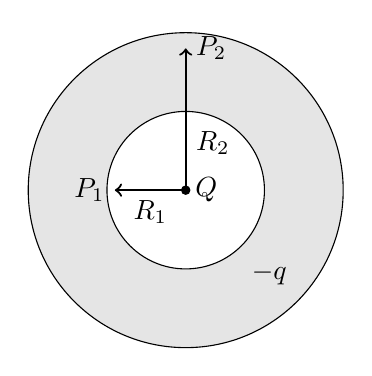
\begin{tikzpicture}
        %% Inner and outer
        \draw[fill=white!90!black] (0,0) circle (2cm);
        \draw[fill=white] (0,0) circle (1cm);
        %% charge
        \draw[fill] (0,0) circle (1.5pt) node[anchor=west] {$Q$};
        \node[anchor=center] at (315:1.5) {$-q$};
        %% Radius
        \draw[thick,->] (0,0) -- (90:1.8cm)
            node[pos=0.33,anchor=west] {$R_2$}
            node[pos=1.00,anchor=west] {$P_2$};
        \draw[thick,->] (0,0) -- (180:0.9cm)
            node[pos=0.50,anchor=north] {$R_1$}
            node[pos=1.00,anchor=east] {$P_1$};
    \end{tikzpicture}
    \end{center}
    The magnitude of the electric field at point $P_1$ a distance $R_1$ from the center is \rule[-0.1pt]{4em}{0.1pt}.
    The magnitude of the electric field at point $P_2$ a distance $R_2$ from the center is \rule[-0.1pt]{4em}{0.1pt}.
    \begin{multicols}{2}
    \begin{choices}
      \correctchoice{zero; zero}
        \wrongchoice{$k\dfrac{Q}{R_1^2}$; zero}
        \wrongchoice{$k\dfrac{Q-q}{R_1^2}$; zero}
        \wrongchoice{zero; $k\dfrac{Q-q}{R_2^2}$}
        \wrongchoice{$k\dfrac{Q-q}{R_1^2}$; $k\dfrac{Q-q}{R_2^2}$}
    \end{choices}
    \end{multicols}
\end{question}
}

\element{aapt}{
\begin{question}{olympiad-1994-q27}
    Resistor $R_4$, as shown in the figure, is a variable resistor.
    \begin{center}
    \ctikzset{bipoles/length=1.00cm}
    \begin{tikzpicture}[scale=1.2]
        \draw (0,0) to[battery,l=$V$] (-2,0) to (-2,3)
                    to [R,l=$R_1$] (0,5) to [R,l=$R_2$] (2,3)
                    to (2,0) -- (0,0);
        \draw (2,3) to[vR,l=$R_4$] (0,1)
                    to[R,l=$R_3$] (-2,3);
        \draw (0,5) to[ammeter] (0,1);
    \end{tikzpicture}
    \end{center}
    In order for there to be no current through the ammeter,
        $R_4$ must be equal to:
    \begin{multicols}{3}
    \begin{choices}
        \wrongchoice{$R_2$}
        \wrongchoice{$R_3$}
        \wrongchoice{$\dfrac{R_1 R_2}{R_3}$}
        \wrongchoice{$\dfrac{R_1 R_3}{R_2}$}
      \correctchoice{$\dfrac{R_2 R_3}{R_1}$}
    \end{choices}
    \end{multicols}
\end{question}
}

\element{aapt}{
\begin{question}{olympiad-1994-q28}
    A resistor $R$ dissipates power $P$ when connected directly to a voltage source $V$,
        as shown in the accompanying figures.
    \begin{center}
    \ctikzset{bipoles/length=0.75cm}
    ~\hfill
    \begin{circuitikz}
        \draw[white] (0,-0.5) -- (2.5,0);
        \draw (0,0) to [battery,l=$V$] (0,2) to (2,2) to [R,l_=$R$] (2,0) to (0,0);
        \node[anchor=west] at (2.1,1) {$P$}; 
    \end{circuitikz}
    \hfill
    \begin{circuitikz}
        \draw (0,0) to (0,1.5) to [battery,l=$V$] (0,3) to (2,3) to [R,l_=$R$] (2,1.5) to [R,l_=$R^{\prime}$] (2,0) to (0,0);
        \node[anchor=west] at (2.1,2.25) {$P/2$}; 
    \end{circuitikz}
    \hfill~
    \end{center}
    What resistance $R^{\prime}$ must be connected in series with $R$ to decrease the power dissipated in $R$ to $\frac{1}{2}P$?
    \begin{multicols}{2}
    \begin{choices}
        \wrongchoice{$\dfrac{R}{2}$}
        \wrongchoice{$\dfrac{R}{\sqrt{2}}$}
        \wrongchoice{$R$}
      \correctchoice{$R\left(\sqrt{2}-1\right)$}
        \wrongchoice{$R\sqrt{2}$}
    \end{choices}
    \end{multicols}
\end{question}
}

\element{aapt}{
\begin{question}{olympiad-1994-q29}
    The infinitely long straight wire carries a conventional current $I$ as shown in the accompanying figure.
    The rectangular loop carries a conventional current $I^{\prime}$ in the counterclockwise direction.
    \begin{center}
    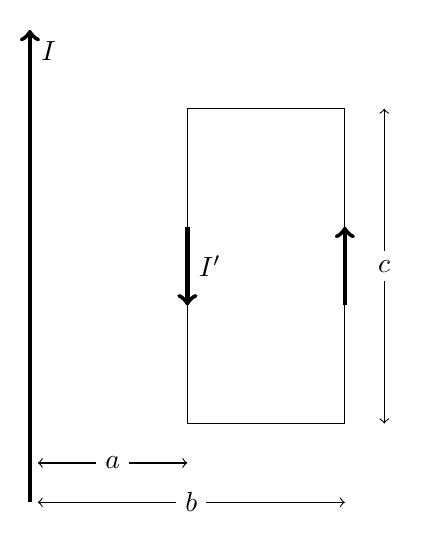
\begin{tikzpicture}
        %% Straight Wire
        \draw[ultra thick,->] (0,-3) -- (0,3) node[anchor=north west] {$I$};
        %% Wire loop
        \draw (2,-2) rectangle (4,+2);
        \draw[ultra thick,->] (2,+0.5) -- (2,-0.5) node[pos=0.5,anchor=west] {$I^{\prime}$};
        \draw[ultra thick,->] (4,-0.5) -- (4,+0.5);
        %% lengths
        \draw[<->] (4.5,-2) -- (4.5,+2) node[pos=0.5,anchor=center,fill=white] {$c$};
        \draw[<->] (0.1,-2.5) -- (2,-2.5) node[pos=0.5,anchor=center,fill=white] {$a$};
        \draw[<->] (0.1,-3) -- (4,-3) node[pos=0.5,anchor=center,fill=white] {$b$};
    \end{tikzpicture}
    \end{center}
    The net force on the rectangular loop is:
    \begin{choices}
      \correctchoice{$\dfrac{\mu II^{\prime} c}{2\pi}\left(\dfrac{1}{a}-\dfrac{1}{b}\right)$ to the right}
        \wrongchoice{$\dfrac{\mu II^{\prime} c}{2\pi}\left(\dfrac{1}{a}+\dfrac{1}{b}\right)$ to the left}
        \wrongchoice{$\dfrac{\mu II^{\prime} c}{2\pi}\left(\dfrac{c}{a}+\dfrac{c}{b}+\dfrac{2\left(b-a\right)}{c}\right)$ to the left}
        \wrongchoice{$\dfrac{\mu II^{\prime} c}{2\pi}\dfrac{2\left(a-b\right)}{c}$ to the right}
        \wrongchoice{zero}
    \end{choices}
\end{question}
}

\element{aapt}{
\begin{question}{olympiad-1994-q30}
    A spatially uniform magnetic field of \SI{0.080}{\tesla} is directed into the plane of the page and perpendicular to it,
        as shown in the accompanying figure.
    A wire loop in the plane of the page has constant area \SI{0.010}{\meter\squared}.
    \begin{center}
    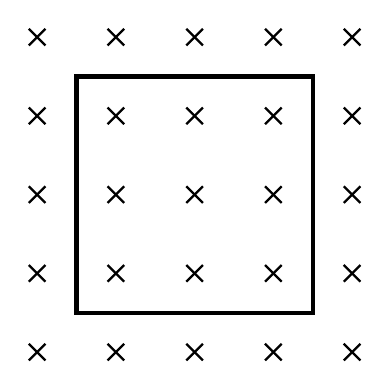
\begin{tikzpicture}
        %% B field into page
        \foreach \x in {1,2,3,4,5}
            \foreach \y in {1,2,3,4,5} {
                \draw[thick] (\x,\y) -- ++(45:0.15);
                \draw[thick] (\x,\y) -- ++(135:0.15);
                \draw[thick] (\x,\y) -- ++(225:0.15);
                \draw[thick] (\x,\y) -- ++(315:0.15);
            }
        %% Wire loop
        \draw[ultra thick] (1.5,1.5) rectangle (4.5,4.5);
    \end{tikzpicture}
    \end{center}
    The magnitude of the magnetic field decreases at a constant rate of \SI{3.0e-4}{\tesla\per\second}.
    What is the magnitude and direction of the induced emf?
    \begin{choices}
      \correctchoice{\SI{3.0e-6}{\volt} clockwise}
        \wrongchoice{\SI{3.0e-6}{\volt} counterclockwise}
        \wrongchoice{\SI{2.4e-5}{\volt} counterclockwise}
        \wrongchoice{\SI{8.0e-4}{\volt} counterclockwise}
        \wrongchoice{\SI{8.0e-4}{\volt} clockwise}
    \end{choices}
\end{question}
}


%% PhysicsOlympiad 1995 Screening Exam
%%----------------------------------------
\element{aapt}{
\begin{question}{olympiad-1995-q01}
    The accompanying figure is a graph of an object's position as a function of time.
    \begin{center}
    \begin{tikzpicture}
        \begin{axis}[
            axis y line=left,
            axis x line=middle,
            axis line style={->},
            xlabel={time},
            xtick=\empty,
            ylabel={position},
            ytick=\empty,
            grid=major,
            xmin=0,xmax=10,
            ymin=-5,ymax=10,
            width=0.8\columnwidth,
            height=0.5\columnwidth,
        ]
        %% NOTE: TODO: make function and labels
        \addplot[line width=1pt,no marks] plot coordinates { (0,0) (2,4) (6,-4) (8,0) };
        \end{axis}
    \end{tikzpicture}
    \end{center}
    Which lettered segment corresponds to a time when the object has a negative acceleration?
    \begin{multicols}{3}
    \begin{choices}
        \wrongchoice{$A$}
        \wrongchoice{$B$}
      \correctchoice{$C$}
        \wrongchoice{$D$}
        \wrongchoice{$E$}
    \end{choices}
    \end{multicols}
\end{question}
}

\element{aapt}{
\begin{question}{olympiad-1995-q02}
    A car is moving at a constant velocity to the right along a straight level highway.
    Just as the car passes a cliff,
        a rock falls straight down in the cliff’s reference system.
    Which of the accompanying curves best depicts the path the rock takes in the car's reference system?
    \begin{multicols}{3}
    \begin{choices}
        \AMCboxDimensions{down=-0.45cm}
        \wrongchoice{
            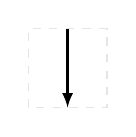
\begin{tikzpicture}
                \draw[dashed,white!90!black] (0,0) rectangle (1,1);
                \draw[thick,-latex] (0.5,1) -- (0.5,0);
            \end{tikzpicture}
        }
        \wrongchoice{
            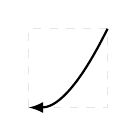
\begin{tikzpicture}
                \draw[dashed,white!90!black] (0,0) rectangle (1,1);
                %\draw[thick,-latex] (1,1) arc(0:-90:1);
                \draw[thick,-latex] (1,1) parabola bend (0,0) (0,0);
            \end{tikzpicture}
        }
        \wrongchoice{
            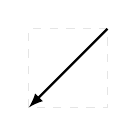
\begin{tikzpicture}
                \draw[dashed,white!90!black] (0,0) rectangle (1,1);
                \draw[thick,-latex] (1,1) -- (0,0);
            \end{tikzpicture}
        }
        %% ANS is E
        \correctchoice{
            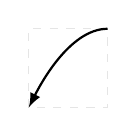
\begin{tikzpicture}
                \draw[dashed,white!90!black] (0,0) rectangle (1,1);
                %\draw[thick,-latex] (1,1) arc(90:180:1);
                \draw[thick,-latex] (1,1) parabola bend (1,1) (0,0);
            \end{tikzpicture}
        }
        \wrongchoice{
            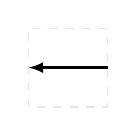
\begin{tikzpicture}
                \draw[dashed,white!90!black] (0,0) rectangle (1,1);
                \draw[thick,-latex] (1,0.5) -- (0,0.5);
            \end{tikzpicture}
        }
    \end{choices}
    \end{multicols}
\end{question}
}

\element{aapt}{
\begin{question}{olympiad-1995-q03}
    Three blocks---1, 2, and 3---rest on a horizontal frictionless surface,
        as shown in the accompanying figure.
    Each block has a mass $m$, and the blocks are connected by massless strings.
    Block 3 is pulled to the right by a force $F$.
    \begin{center}
    \begin{tikzpicture}
        %% Floor
        \node[anchor=north,fill,pattern=north east lines,minimum width=8cm, minimum height=0.05cm] at (-1.5,0) {};
        \draw (-5.5,0) -- (2.5,0);
        %% Blocks
        \node[anchor=south,minimum size=1cm,draw,fill=white!90!black] (A) at (0,0) {$m$};
        \node[anchor=south,minimum size=1cm,draw,fill=white!90!black] (B) at (-2,0) {$m$};
        \node[anchor=south,minimum size=1cm,draw,fill=white!90!black] (C) at (-4,0) {$m$};
        %% Labels
        \node[anchor=south] at (A.north) {3};
        \node[anchor=south] at (B.north) {2};
        \node[anchor=south] at (C.north) {1};
        %% Strings
        \draw[thick] (A.west) -- (B.east);
        \draw[thick] (B.west) -- (C.east);
        %% Force
        \draw[thick,->] (A.east) -- ++(0:1.5cm) node[pos=0.5,anchor=south] {$F$};
    \end{tikzpicture}
    \end{center}
    The resultant force on block 2 is:
    \begin{multicols}{3}
    \begin{choices}
        \wrongchoice{zero}
      \correctchoice{$\dfrac{F}{3}$}
        \wrongchoice{$\dfrac{F}{2}$}
        \wrongchoice{$\dfrac{2F}{3}$}
        \wrongchoice{$F$}
    \end{choices}
    \end{multicols}
\end{question}
}

\element{aapt}{
\begin{question}{olympiad-1995-q04}
    Which solid vector in the accompanying figures best represents the acceleration of a pendulum mass at an intermediate point in its swing?
    \begin{multicols}{2}
    \begin{choices}
        \AMCboxDimensions{down=-1cm}
        \wrongchoice{
            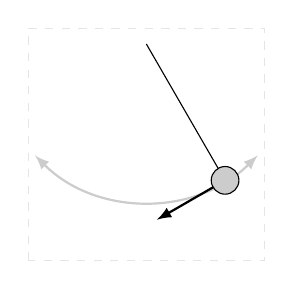
\begin{tikzpicture}
                \draw[dashed,white!90!black] (-1.5,-2.75) rectangle (1.5,0.2);
                %% string
                \draw (0,0) -- (300:2);
                %% path
                \draw[thick,white!80!black,latex-latex] (225:2) arc(225:315:2);
                %% arrows
                \draw[thick,-latex] (300:2) -- ++(210:1);
                %% bob
                \draw[fill=white!80!black] (300:2) circle (5pt);
            \end{tikzpicture}
        }
        \wrongchoice{
            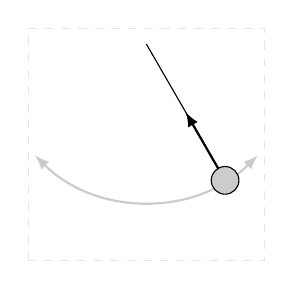
\begin{tikzpicture}
                \draw[dashed,white!90!black] (-1.5,-2.75) rectangle (1.5,0.2);
                %% string
                \draw (0,0) -- (300:2);
                %% path
                \draw[thick,white!80!black,latex-latex] (225:2) arc(225:315:2);
                %% arrows
                \draw[thick,-latex] (300:2) -- ++(120:1);
                %% bob
                \draw[fill=white!80!black] (300:2) circle (5pt);
            \end{tikzpicture}
        }
        \wrongchoice{
            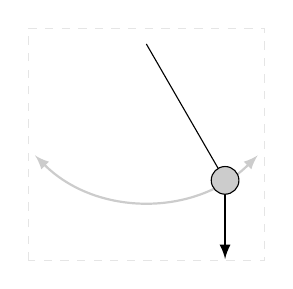
\begin{tikzpicture}
                \draw[dashed,white!90!black] (-1.5,-2.75) rectangle (1.5,0.2);
                %% string
                \draw (0,0) -- (300:2);
                %% path
                \draw[thick,white!80!black,latex-latex] (225:2) arc(225:315:2);
                %% arrows
                \draw[thick,-latex] (300:2) -- ++(270:1);
                %% bob
                \draw[fill=white!80!black] (300:2) circle (5pt);
            \end{tikzpicture}
        }
        %% ANS is D
        \correctchoice{
            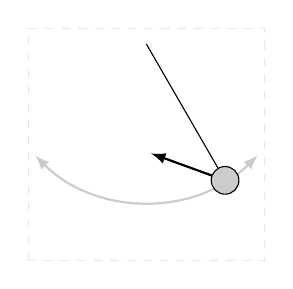
\begin{tikzpicture}
                \draw[dashed,white!90!black] (-1.5,-2.75) rectangle (1.5,0.2);
                %% string
                \draw (0,0) -- (300:2);
                %% path
                \draw[thick,white!80!black,latex-latex] (225:2) arc(225:315:2);
                %% arrows
                \draw[thick,-latex] (300:2) -- ++(160:1);
                %% bob
                \draw[fill=white!80!black] (300:2) circle (5pt);
            \end{tikzpicture}
        }
        \wrongchoice{
            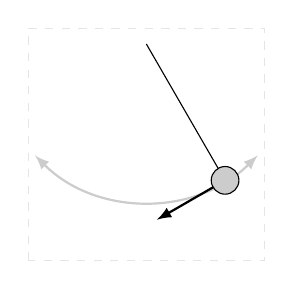
\begin{tikzpicture}
                \draw[dashed,white!90!black] (-1.5,-2.75) rectangle (1.5,0.2);
                %% string
                \draw (0,0) -- (300:2);
                %% path
                \draw[thick,white!80!black,latex-latex] (225:2) arc(225:315:2);
                %% arrows
                \draw[thick,-latex] (300:2) -- ++(210:1);
                %% bob
                \draw[fill=white!80!black] (300:2) circle (5pt);
            \end{tikzpicture}
        }
    \end{choices}
    \end{multicols}
\end{question}
}

\element{aapt}{
\begin{question}{olympiad-1995-q05}
    A mass attached to a horizontal massless spring is displaced \SI{16}{\centi\meter} to the right of its equilibrium position and released from rest.
    At its \SI{16}{\centi\meter} extension,
        the spring-mass system has \SI{1.28}{\joule} of potential energy.
    \begin{center}
    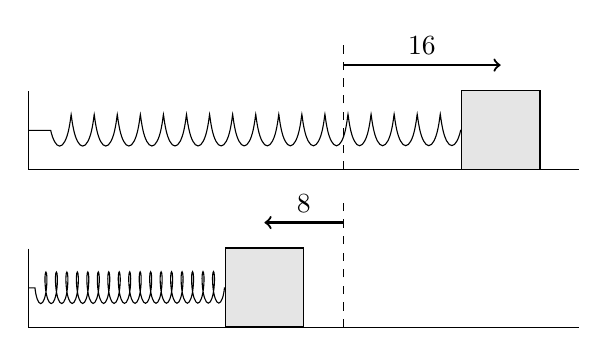
\begin{tikzpicture}
        \begin{scope}[yshift=1cm]
            %% Floor and Wall
            \draw (0,1) -- (0,0) -- (7,0);
            %% block
            \node[draw,fill=white!90!black,minimum size=1cm,anchor=south] (A) at (6,0) {};
            %% Spring
            \draw[decoration={aspect=0.2,segment length=2.93mm,amplitude=2mm,coil},decorate] (A.west) -- (0,0.5);
            %% midway
            \draw[dashed] (4,0) -- (4,1.66);
            \draw[thick,->] (4,1.33) -- (6,1.33) node[pos=0.5,anchor=south] {\SI{16}{\centi\meter}};
        \end{scope}
        \begin{scope}[yshift=-1cm]
            %% Floor and Wall
            \draw (0,1) -- (0,0) -- (7,0);
            %% block
            \node[draw,fill=white!90!black,minimum size=1cm,anchor=south] (A) at (3,0) {};
            %% Spring
            \draw[decoration={aspect=0.2,segment length=1.33mm,amplitude=2mm,coil},decorate] (A.west) -- (0,0.5);
            %% midway
            \draw[dashed] (4,0) -- (4,1.66);
            \draw[thick,->] (4,1.33) -- (3,1.33) node[pos=0.5,anchor=south] {\SI{8}{\centi\meter}};
        \end{scope}
    \end{tikzpicture}
    \end{center}
    Upon release, it slides across a rough surface and comes momentarily to rest \SI{8}{\centi\meter} to the left of its equilibrium position.
    How much mechanical energy was dissipated by friction?
    \begin{multicols}{3}
    \begin{choices}
        \wrongchoice{\SI{0.16}{\joule}}
        \wrongchoice{\SI{0.32}{\joule}}
        \wrongchoice{\SI{0.64}{\joule}}
      \correctchoice{\SI{0.96}{\joule}}
        \wrongchoice{\SI{1.12}{\joule}}
    \end{choices}
    \end{multicols}
\end{question}
}

\element{aapt}{
\begin{question}{olympiad-1995-q06}
    Two identical masses $m$ are connected to a massless string which is hung over two frictionless pulleys as shown.
    \begin{center}
    \begin{tikzpicture}
        %% Ceiling
        \node[anchor=south,fill,pattern=north east lines,minimum width=8cm, minimum height=0.05cm] at (0,0) {};
        \draw (-4,0) -- (4,0);
        %% Mass Left
        \node[draw,anchor=north,minimum size=1cm,fill=white!90!black,rounded corners=0.5ex] (A) at (-2.5,-2.5) {$m$};
        %% Mass Right
        \node[draw,anchor=north,minimum size=1cm,fill=white!90!black,rounded corners=0.5ex] (B) at (+2.5,-2.5) {$m$};
        %% Rope
        \draw[very thick] (A.north) -- (-2.5,-1) arc(180:90:0.5) -- (+2,-0.5) arc(90:0:0.5) -- (B.north);
        %% Pulley Left
        \draw (-2,-1) circle (0.5cm);
        \draw[fill=white!90!black] (-2.2,0) -- (-2.1,-1.1) arc(190:350:0.1) -- (-1.8,0) -- cycle;
        \draw[fill] (-2,-1) circle (1pt);
        %% Pulley Right
        \draw (+2,-1) circle (0.5cm);
        \draw[fill=white!90!black] (+1.8,0) -- (+1.9,-1.1) arc(190:350:0.1) -- (+2.2,0) -- cycle;
        \draw[fill] (+2,-1) circle (1pt);
    \end{tikzpicture}
    \end{center}
    If everything is at rest,
        what is the tension in the cord?
    \begin{choices}
        \wrongchoice{Less than $mg$.}
      \correctchoice{Exactly $mg$.}
        \wrongchoice{More than $mg$ but less than $2mg$.}
        \wrongchoice{Exactly $2mg$.}
        \wrongchoice{More than $2mg$.}
    \end{choices}
\end{question}
}

\element{aapt}{
\begin{question}{olympiad-1995-q07}
    Car $A$ and car $B$ are both traveling down a straight highway at \SI{25}{\meter\per\second} (about \SI{56}{\mile\per\hour}).
    Car $A$ is only \SI{6.0}{\meter} behind car $B$.
    The driver of car $B$ brakes,
        slowing down with a constant acceleration of \SI{2.0}{\meter\per\second\squared}.
    After a time \SI{1.2}{\second},
        the driver of car $A$ begins to brake,
        also at \SI{2.0}{\meter\per\second\squared}.
    What is the relative velocity of the two cars when they collide?
    Hint: Both cars are still moving forward when they collide.
    \begin{multicols}{3}
    \begin{choices}
      \correctchoice{\SI{2.4}{\meter\per\second}}
        \wrongchoice{\SI{5.0}{\meter\per\second}}
        \wrongchoice{\SI{9.5}{\meter\per\second}}
        \wrongchoice{\SI{21}{\meter\per\second}}
        \wrongchoice{\SI{24}{\meter\per\second}}
    \end{choices}
    \end{multicols}
\end{question}
}

\element{aapt}{
\begin{question}{olympiad-1995-q08}
    %% NOTE: make self contained
    During the collision between car $A$ and car $B$ described in Problem \#7 above,
        which car experiences the greater change in momentum?
    \begin{choices}
        \wrongchoice{The more massive car.}
        \wrongchoice{The less massive car.}
        \wrongchoice{Car $A$ because its velocity at the start of the collision is greater.}
        \wrongchoice{Car $B$ because its velocity at the start of the collision is less.}
      \correctchoice{Both cars experience the same magnitude of momentum change.}
    \end{choices}
\end{question}
}

\element{aapt}{
\begin{question}{olympiad-1995-q09}
    A \SI{70}{\kilo\gram} hunter ropes a \SI{350}{\kilo\gram} polar bear.
    Both are initially at rest,
        \SI{30}{\meter} apart on a frictionless and level ice surface.
    When the hunter pulls the polar bear to him,
        the polar bear will move:
    \begin{multicols}{3}
    \begin{choices}
      \correctchoice{\SI{5}{\meter}}
        \wrongchoice{\SI{6}{\meter}}
        \wrongchoice{\SI{15}{\meter}}
        \wrongchoice{\SI{24}{\meter}}
        \wrongchoice{\SI{25}{\meter}}
    \end{choices}
    \end{multicols}
\end{question}
}

\element{aapt}{
\begin{question}{olympiad-1995-q10}
    A bullet of mass $m$ is fired at a block of mass $M$ initially at rest.
    The bullet, moving at an initial speed $v$,
        embeds itself in the block.
    The speed of the block after the collision is:
    \begin{multicols}{2}
    \begin{choices}
        \wrongchoice{$\dfrac{Mv}{M+m}$}
        \wrongchoice{$\dfrac{\left(M+m\right)v}{m}$}
        \wrongchoice{$v\sqrt{\dfrac{m}{M+m}}$}
        \wrongchoice{$v\sqrt{\dfrac{M+m}{m}}$}
      \correctchoice{$\dfrac{mv}{M+m}$}
    \end{choices}
    \end{multicols}
\end{question}
}

\element{aapt}{
\begin{question}{olympiad-1995-q11}
    The driver of a \SI{1000}{\kilo\gram} car tries to turn through a circle of radius \SI{100}{\meter} on an unbanked curve at a speed of \SI{10}{\meter\per\second}.
    The maximum frictional force between the tires and the slippery road is \SI{900}{\newton}.
    The car will:
    \begin{choices}
        \wrongchoice{Slide into the inside of the curve.}
        \wrongchoice{Make the turn.}
        \wrongchoice{Slow down due to the centrifugal force.}
        \wrongchoice{Make the turn only if it speeds up.}
      \correctchoice{Slide off to the outside of the curve.}
    \end{choices}
\end{question}
}

\element{aapt}{
\begin{question}{olympiad-1995-q12}
    A solid cylinder weighing \SI{200}{\newton} has a fixed axis and a string wrapped around it.
    The string is pulled with a force equal to the weight of the cylinder.
    The acceleration of the string is approximately:
    \begin{multicols}{3}
    \begin{choices}
        \wrongchoice{\SI{10}{\meter\per\second\squared}}
      \correctchoice{\SI{20}{\meter\per\second\squared}}
        \wrongchoice{\SI{30}{\meter\per\second\squared}}
        \wrongchoice{\SI{40}{\meter\per\second\squared}}
        \wrongchoice{\SI{50}{\meter\per\second\squared}}
    \end{choices}
    \end{multicols}
\end{question}
}

\element{aapt}{
\begin{question}{olympiad-1995-q13}
    A spinning ice skater has an initial kinetic energy $\frac{1}{2}I\omega^2$.
    She pulls in her outstretched arms,
        decreasing her moment of inertia to $\frac{1}{4}I$.
    Her new angular speed is:
    \begin{multicols}{3}
    \begin{choices}
        \wrongchoice{$\dfrac{1}{4}\omega$}
        \wrongchoice{$\dfrac{1}{2}\omega$}
        \wrongchoice{$\omega$}
        \wrongchoice{$2\omega$}
      \correctchoice{$4\omega$}
    \end{choices}
    \end{multicols}
\end{question}
}

\element{aapt}{
\begin{question}{olympiad-1995-q14}
    A heavy rod of length $L$ and weight $W$ is suspended horizontally by two vertical ropes as shown below. The first rope is attached to the left end of the rod while the second rope is attached a distance $\frac{1}{4}L$ from the right end.
    \begin{center}
    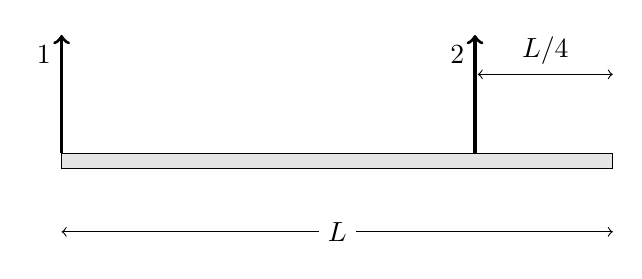
\begin{tikzpicture}[xscale=1.75]
        %% heavy rod
        \draw[fill=white!90!black] (-2,0) rectangle (2,-0.2);
        %% ropes
        \draw[very thick,->] (-2,0) -- ++(90:1.5) node[anchor=north east] {1};
        \draw[very thick,->] (+1,0) -- ++(90:1.5) node[anchor=north east] {2};
        %% labels
        \draw[<->] (-2,-1) -- (2,-1) node[pos=0.5,anchor=center,fill=white] {$L$};
        \draw[<->] (2,1) -- (1.02,1) node[pos=0.5,anchor=south] {$L/4$};
    \end{tikzpicture}
    \end{center}
    The tension in the second rope is:
    \begin{multicols}{3}
    \begin{choices}
        \wrongchoice{$\dfrac{1}{2}W$}
        \wrongchoice{$\dfrac{1}{4}W$}
        \wrongchoice{$\dfrac{1}{3}W$}
        \wrongchoice{$\dfrac{2}{3}W$}
        \wrongchoice{$W$}
    \end{choices}
    \end{multicols}
\end{question}
}

\element{aapt}{
\begin{question}{olympiad-1995-q15}
    A block of ice with mass $m$ falls into a lake.
    After impact, a mass of ice $m/5$ melts.
    Both the block of ice and the lake have a temperature of \SI{0}{\degreeCelsius}.
    If $L$ represents the heat of fusion,
        the minimum distance the ice fell is:
    \begin{multicols}{3}
    \begin{choices}
      \correctchoice{$\dfrac{L}{5g}$}
        \wrongchoice{$\dfrac{5L}{g}$}
        \wrongchoice{$\dfrac{gL}{5m}$}
        \wrongchoice{$\dfrac{mL}{5g}$}
        \wrongchoice{$\dfrac{5gL}{m}$}
    \end{choices}
    \end{multicols}
\end{question}
}

\element{aapt}{
\begin{question}{olympiad-1995-q16}
    Which of the accompanying PV diagrams best represents an isothermal (constant temperature) process?
    \begin{multicols}{3}
    \begin{choices}
        %% NOTE: ANS is B
        \wrongchoice{
            \begin{tikzpicture}
                %% NOTE: TODO: pgfplots
            \end{tikzpicture}
        }
    \end{choices}
    \end{multicols}
\end{question}
}

\element{aapt}{
\begin{question}{olympiad-1995-q17}
    If the heat is added at constant volume,
        \SI{6300}{\joule} of heat are required to raise the temperature of an ideal gas by \SI{150}{\kelvin}.
    If instead, the heat is added at constant pressure,
        \SI{8800}{\joule} are needed for the same temperature change.
    When the temperature of the gas changes by \SI{150}{\kelvin},
        the internal energy of the gas changes by:
    \begin{multicols}{3}
    \begin{choices}
        \wrongchoice{\SI{2500}{\joule}}
      \correctchoice{\SI{6300}{\joule}}
        \wrongchoice{\SI{8800}{\joule}}
        \wrongchoice{\SI{11 300}{\joule}}
        \wrongchoice{\SI{15 100}{\joule}}
    \end{choices}
    \end{multicols}
\end{question}
}

\element{aapt}{
\begin{question}{olympiad-1995-q18}
    A firecracker exploding on the surface of a lake is heard as two sounds---a time interval $t$ apart---by the paddler of a nearby canoe.
    Sound travels with a speed $u$ in water and a speed $v$ in air.
    The distance from the exploding firecracker to the canoe is:
    \begin{multicols}{3}
    \begin{choices}
        \wrongchoice{$\dfrac{uvt}{u+v}$}
        \wrongchoice{$\dfrac{t\left(u+v\right)}{uv}$}
        \wrongchoice{$\dfrac{t\left(u-v\right)}{uv}$}
        \wrongchoice{$vt$}
      \correctchoice{$\dfrac{uvt}{u-v}$}
    \end{choices}
    \end{multicols}
\end{question}
}

\element{aapt}{
\begin{question}{olympiad-1995-q19}
    Two interfering waves have the same wavelength, frequency, and amplitude.
    They are traveling in the same direction but are 90º out of phase.
    Compared to the individual waves, the resultant wave will have the same:
    \begin{choices}
        \wrongchoice{amplitude and velocity but different wavelength.}
        \wrongchoice{amplitude and wavelength but different velocity.}
      \correctchoice{wavelength and velocity but different amplitude.}
        \wrongchoice{amplitude and frequency but different velocity.}
        \wrongchoice{frequency and velocity but different wavelength.}
    \end{choices}
\end{question}
}

\element{aapt}{
\begin{question}{olympiad-1995-q20}
    An organ pipe which is open at both ends resonates with fundamental frequency \SI{300}{\hertz}.
    If one end of the pipe is closed,
        it will resonate with a fundamental frequency of:
    \begin{multicols}{3}
    \begin{choices}
        \wrongchoice{\SI{75}{\hertz}}
      \correctchoice{\SI{150}{\hertz}}
        \wrongchoice{\SI{300}{\hertz}}
        \wrongchoice{\SI{600}{\hertz}}
        \wrongchoice{\SI{1200}{\hertz}}
    \end{choices}
    \end{multicols}
\end{question}
}

\element{aapt}{
\begin{question}{olympiad-1995-q21}
    You are given two lenses,
        a converging lens with focal length \SI{+10}{\centi\meter} and a diverging lens with focal length \SI{-20}{\centi\meter}.
    Which of the following would produce a virtual image that is larger than the object?
    \begin{choices}
      \correctchoice{Placing the object \SI{5}{\centi\meter} from the converging lens.}
        \wrongchoice{Placing the object \SI{15}{\centi\meter} from the converging lens.}
        \wrongchoice{Placing the object \SI{25}{\centi\meter} from the converging lens.}
        \wrongchoice{Placing the object \SI{15}{\centi\meter} from the diverging lens.}
        \wrongchoice{Placing the object \SI{25}{\centi\meter} from the diverging lens.}
    \end{choices}
\end{question}
}

\element{aapt}{
\begin{question}{olympiad-1995-q22}
    Light shining through two very narrow slits produces an interference maximum at point $P$ when the entire apparatus is in air (see accompanying figure).
    \begin{center}
    \begin{tikzpicture}
        %% NOTE: TODO: tikz
        %% Two slits
        \draw[very thick] (0,-1.5) -- (0,1.5);
        \draw[white,fill=white] (0,+1) circle (4pt);
        \draw[white,fill=white] (0,-1) circle (4pt);
        \draw[<->] (-1,-1) -- (-1,+1) node[pos=0.5,anchor=center,fill=white] {$d$};
        %% point P
        \draw[fill] (6,2) circle (1pt) node[anchor=south] {$P$};
        \draw (0,+1) -- (6,2);
        \draw (0,-1) -- (6,2);
        %% distance x
        \draw[<->] (6,0) -- (6,1.95) node[pos=0.5,anchor=center,fill=white] {$x$};
        \draw[dashed] (-0.2,0) -- (6.2,0);
        \draw[dashed] (0,0) -- (6,2);
        \draw[<->] (1.5,0) arc(0:18.4:1.5) node[pos=0.5,anchor=west] {$\theta$};
    \end{tikzpicture}
    \end{center}
    For the interference maximum represented,
        light through the bottom slit travels one wavelength further than light through the top slit before reaching point $P$.
    If the entire apparatus is immersed in water,
        the angle $\theta$ to the interference maximum:
    \begin{choices}
        \wrongchoice{is unchanged}
        \wrongchoice{decreases because the frequency decreases.}
        \wrongchoice{decreases because the wavelength decreases.}
        \wrongchoice{increases because the frequency increases.}
        \wrongchoice{increases because the wavelength increases.}
    \end{choices}
\end{question}
}

\element{aapt}{
\begin{question}{olympiad-1995-q23}
    The magnitude of the field due to an infinite plate of charge is $\sigma/(2\varepsilon_0)$,
        where $\sigma$ is the charge per unit area and $\varepsilon_0$ is the vacuum permittivity.
    The figure below depicts three infinite plates of perpendicular to the plane of the page with charge per unit area $\sigma_1$, $+2\sigma_1$, and $-\sigma_1$.
    \begin{center}
    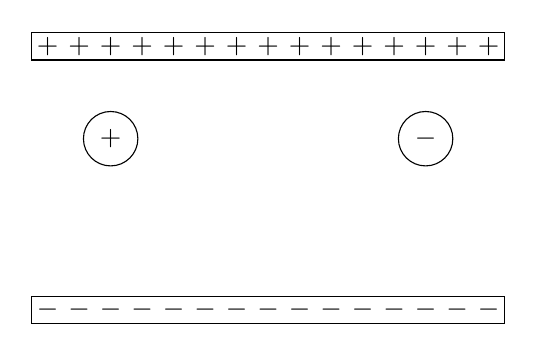
\begin{tikzpicture}
        %% NOTE: TODO: tikz
        %% This was copied from elsewhere, make vertical, not horizontal
        %% Charges
        \node[draw,circle,anchor=center] at (+1,2) {$+$};
        \node[draw,circle,anchor=center] at (+5,2) {$-$};
        %% Top
        \draw (0,0) rectangle (6,-1em);
        \foreach \x in {2,6,...,58}
            \node[anchor=center] at (\x mm,3cm+0.5em) {$+$};
        %% Bottom
        \draw (0,3) rectangle (6,3cm+1em);
        \foreach \x in {2,6,...,58}
            \node[anchor=center] at (\x mm,-0.5em) {$-$};
    \end{tikzpicture}
    \end{center}
    The total field at the point labeled $X$ is:
    \begin{multicols}{2}
    \begin{choices}
        \wrongchoice{$\dfrac{4\sigma_1}{2\varepsilon_0}$ to the left}
        \wrongchoice{$\dfrac{\sigma_1}{2\varepsilon_0}$ to the left}
        \wrongchoice{zero}
        \wrongchoice{$\dfrac{\sigma_1}{2\varepsilon_0}$ to the right}
        \wrongchoice{$\dfrac{4\sigma_1}{2\varepsilon_0}$ to the right}
    \end{choices}
    \end{multicols}
\end{question}
}

\element{aapt}{
\begin{question}{olympiad-1995-q24}
    There are three conducting spheres of identical diameter,
        shown below.
    \begin{center}
    \begin{tikzpicture}
        %% NOTE: TODO: tikz
    \end{tikzpicture}
    \end{center}
    Spheres 1 and 2 are separated by a distance that is large compared to their diameter.
    They have equal charges and repel each other with an electrostatic force $F$.
    Sphere 3 is initially uncharged and has an insulated handle.
    It is touched first to sphere 1, then to sphere 2, and then removed.
    If the distance between spheres 1 and 2 has not changed, the force between these two spheres is:
    \begin{multicols}{3}
    \begin{choices}
        \wrongchoice{zero}
        \wrongchoice{$\dfrac{1}{16} F$}
        \wrongchoice{$\dfrac{1}{4} F$}
        \wrongchoice{$\dfrac{3}{8} F$}
        \wrongchoice{$\dfrac{1}{2} F$}
    \end{choices}
    \end{multicols}
\end{question}
}

\element{aapt}{
\begin{questionmult}{olympiad-1995-q25}
    Two conducting spheres, $A$ of radius $a$ and $B$ of radius $b$,
        are shown in the accompanying figure.
    \begin{center}
    \begin{tikzpicture}
        %% NOTE: TODO: tikz
    \end{tikzpicture}
    \end{center}
    Both are positively charged and isolated from their surroundings.
    They had been connected by a conducting wire but the wire has been removed.
    Assuming the potential an infinite distance away is zero,
        which of the following statements about the spheres are true:
    \begin{choices}[o]
        %% A. i and iv B. i and vi C. ii and vi    D. iii and iv   E. iii and v
        \wrongchoice{Sphere $A$ is at the higher potential.}
        \wrongchoice{Sphere $B$ is at the higher potential.}
      \correctchoice{Both spheres have the same potential.}
      \correctchoice{Sphere $A$ has the larger charge.}
        \wrongchoice{Sphere $B$ has the larger charge.}
        \wrongchoice{Both spheres have the same charge.}
    \end{choices}
\end{questionmult}
}

\element{aapt}{
\begin{question}{olympiad-1995-q26}
    The accompanying figure shows two concentric spherical shells isolated from each other.
    \begin{center}
    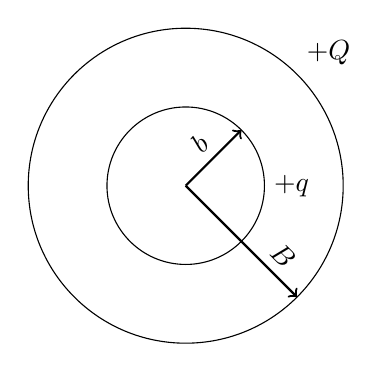
\begin{tikzpicture}
        %% small sphere
        \draw (0,0) circle (1cm);
        \draw[thick,->] (0,0) -- (45:1) node[pos=0.5,anchor=south,rotate=45] {$b$};
        \node[anchor=west] at (0:1) {$+q$};
        %% large sphere
        \draw (0,0) circle (2cm);
        \draw[thick,->] (0,0) -- (315:2) node[pos=0.75,anchor=south,rotate=-45] {$B$};
        \node[anchor= south west] at (45:2) {$+Q$};
    \end{tikzpicture}
    \end{center}
    The smaller shell has radius $b$ and net charge $+q$.
    The larger shell has radius $B$ and net charge $+Q$.
    Assume that the potential is zero at an infinite distance from the shells.
    If $R$ is the distance from the common center,
        the highest electric potential $V$ occurs:
    \begin{choices}
        \wrongchoice{only at $R=0$, where $V$ is infinite}
      \correctchoice{anywhere $R\geq b$, where $V$ is constant}
        \wrongchoice{in the region $b < R < B$.}
        \wrongchoice{immediately outside the larger shell; $V$ is zero everywhere within it.}
        \wrongchoice{far away from the shells; $V$ increases with distance.}
    \end{choices}
\end{question}
}

\element{aapt}{
\begin{question}{olympiad-1995-q27}
    In the circuit represented below,
    \begin{center}
    \ctikzset{bipoles/length=0.75cm}
    \begin{circuitikz}
        \draw[ultra thick,-latex] (0,0.5) -- (0,1.5) node[pos=0.5,anchor=east] {$I$};
        \draw (0,0) to (0,1.5) to [battery,l=$V$] (0,3) to [R,l=$R$] (2,3) to [R,l=$R$] (4,3) to [R,l=$R$] (4,0) to (0,0);
        \draw (2,0) to [battery,l=$V$] (2,1.5) to [R,l=$R$] (2,3);
    \end{circuitikz}
    \end{center}
    the current $I$ equals:
    \begin{multicols}{3}
    \begin{choices}
      \correctchoice{$\dfrac{V}{5R}$}
        \wrongchoice{$\dfrac{V}{4R}$}
        \wrongchoice{$\dfrac{2V}{5R}$}
        \wrongchoice{$\dfrac{V}{2R}$}
        \wrongchoice{$\dfrac{2V}{R}$}
    \end{choices}
    \end{multicols}
\end{question}
}

\element{aapt}{
\begin{question}{olympiad-1995-q28}
    %%Refer to the following information for the next two questions.
    In the following diagram, $L_1$, $L_2$, $L_3$, and $L_4$ are identical light bulbs.
    There are six voltmeters connected to the circuit as shown.
    Assume that the voltmeters do not effect the circuit.
    \begin{center}
    \ctikzset{bipoles/length=1.00cm}
    \begin{circuitikz}[scale=0.80]
        %% NOTE: TODO: circuittikz
        \draw (0,0) to (0,2) to [battery] (0,4) to [R,l=$L_1$] (4,4) to (8,4) to [R,l=$L_3$] (8,2) to  [R,l=$L_4$] (8,0) to (0,0);
        \draw (4,0) to [R,l=$L_2$] (4,4);
    \end{circuitikz}
    \end{center}
    Which of the following combinations are equal to $V_0$?
    \begin{multicols}{3}
    \begin{choices}
        \wrongchoice{$V_1 + V_3$}
        \wrongchoice{$V_2 + V_3 + V_4$}
      \correctchoice{$V_1 + V_5$}
        \wrongchoice{$V_3 + V_4$}
        \wrongchoice{$V_1 + V_4$}
    \end{choices}
    \end{multicols}
\end{question}
}

\element{aapt}{
\begin{question}{olympiad-1995-q29}
    %%Refer to the following information for the next two questions.
    In the following diagram, $L_1$, $L_2$, $L_3$, and $L_4$ are identical light bulbs.
    There are six voltmeters connected to the circuit as shown.
    Assume that the voltmeters do not effect the circuit.
    \begin{center}
    \begin{tikzpicture}
        %% NOTE: TODO: circuittikz
    \end{tikzpicture}
    \end{center}
    If $L_3$ were to burn out,
        opening the circuit, which voltmeter(s) would read zero volts?
    %\begin{multicols}{2}
    \begin{choices}
        %% NOTE: questionmult?
        \wrongchoice{None would read zero.}
        \wrongchoice{only $V_3$}
      \correctchoice{only $V_4$}
        \wrongchoice{only $V_3$, $V_4$, and $V_5$}
        \wrongchoice{they would all read zero}
    \end{choices}
    %\end{multicols}
\end{question}
}

\element{aapt}{
\begin{question}{olympiad-1995-q30}
    Identical currents flow in two perpendicular wires,
        as shown in the accompanying figure.
    The wires are very close but do not touch.
    \begin{center}
    \begin{tikzpicture}
        %% NOTE: TODO: circuittikz
    \end{tikzpicture}
    \end{center}
    The magnetic field can be zero:
    \begin{choices}
        \wrongchoice{at a point in region 1 only}
        \wrongchoice{at a point in region 2 only}
        \wrongchoice{at points in both regions 1 and 2}
        \wrongchoice{at points in both regions 1 and 4}
      \correctchoice{at points in both regions 2 and 4}
    \end{choices}
\end{question}
}


%% PhysicsOlympiad 1996 Screening Exam
%%----------------------------------------
\element{aapt}{
\begin{question}{olympiad-1996-q01}
    An object is projected straight upward from ground level with a velocity of \SI{50}{\meter\per\second}.
    Ignoring air resistance,
        it will return to ground level in approximately:
    \begin{multicols}{3}
    \begin{choices}
        \wrongchoice{\SI{2.5}{\second}}
        \wrongchoice{\SI{5.0}{\second}}
        \wrongchoice{\SI{7.5}{\second}}
      \correctchoice{\SI{10}{\second}}
        \wrongchoice{\SI{15}{\second}}
    \end{choices}
    \end{multicols}
\end{question}
}

\element{aapt}{
\begin{question}{olympiad-1996-q02}
    A jogger runs with constant speed $v$ through a forest of pine trees.
    A pine cone starts to fall from a height h when the jogger is directly below it.
    How far behind the jogger will the pine cone land?
    \begin{multicols}{3}
    \begin{choices}
      \correctchoice{$\sqrt{\dfrac{2hv^2}{g}}$}
        \wrongchoice{$\sqrt{\dfrac{hv^2}{g}}$}
        \wrongchoice{$\dfrac{gh^2}{2v^2}$}
        \wrongchoice{$\dfrac{2gh^2}{v^2}$}
        \wrongchoice{$\dfrac{v^2}{2g}$}
    \end{choices}
    \end{multicols}
\end{question}
}

\element{aapt}{
\begin{question}{olympiad-1996-q03}
    A ball is thrown downward with speed \SI{15}{\meter\per\second} from the roof of a \SI{30}{\meter} building.
    At the same instant a ball is thrown upward with speed \SI{15}{\meter\per\second} from ground level.
    Relative to ground level,
        the two balls pass each other at a height of:
    \begin{multicols}{3}
    \begin{choices}
        \wrongchoice{zero}
        \wrongchoice{\SI{5.0}{\meter}}
      \correctchoice{\SI{10}{\meter}}
        \wrongchoice{\SI{15}{\meter}}
        \wrongchoice{\SI{20}{\meter}}
    \end{choices}
    \end{multicols}
\end{question}
}

\element{aapt}{
\begin{question}{olympiad-1996-q04}
    A swimmer can swim with a velocity of \SI{1.0}{\meter\per\second} in still water.
    The swimmer wishes to swim directly across a river with a current of \SI{0.50}{\meter\per\second} directed from upstream to downstream.
    To end up directly across the river the swimmer must head at an angle of:
    \begin{choices}
        \wrongchoice{$\tan^{-1}\left(\dfrac{1}{2}\right)$ upstream.}
      \correctchoice{$\sin^{-1}\left(\dfrac{1}{2}\right)$ upstream.}
        \wrongchoice{directly across the river.}
        \wrongchoice{$\sin^{-1}\left(\dfrac{1}{2}\right)$ downstream}
        \wrongchoice{$\tan^{-1}\left(\dfrac{1}{2}\right)$ downstream}
    \end{choices}
\end{question}
}

\element{aapt}{
\begin{question}{olympiad-1996-q05}
    What is the tension $T$ in the rope if the \SI{10}{\newton} weight is moving upward with constant velocity?
    \begin{center}
    \begin{tikzpicture}
        %% Ceiling
        \node[anchor=south,fill,pattern=north east lines,minimum width=6cm, minimum height=0.05cm] at (-1,0) {};
        \draw (-4,0) -- (2,0);
        %% Rope
        \draw[very thick,->] (+1.0,0) -- (+1,-3) arc(0:-180:0.5) -- (0,-1) arc(0:135:0.5) -- ++(225:3.5) node[pos=1.0,anchor=south,yshift=0.05cm] {$T$};
        \draw[dashed] (-0.5,-0.5) ++(-0.3535,-0.1464) ++(225:3) -- ++(0:2);
        \draw[thick,<->] (-0.5,-0.5) ++(-0.3535,-0.1464) ++(225:3) ++(0:1.5) arc(0:45:1.5) node[pos=0.5,anchor=west] {\ang{45}};
        %% first pulley
        \draw[thick] (-0.5,-1) circle (0.5);
        \draw[fill=white!90!black] (-0.8,0) -- (-0.7,-1.1) arc(190:350:0.2) -- (-0.2,0) --cycle;
        \draw[fill] (-0.5,-1) circle (1.5pt);
        %% second pulley
        \draw[thick] (0.5,-3) circle (0.50);
        \draw[fill] (0.5,-3) circle (1.5pt);
        %% Masses
        \node[draw,fill=white!90!black,rectangle,rounded corners=1ex,minimum size=1.2cm,anchor=north] (B) at (0.5,-4) {\SI{10}{\newton}};
        \draw[thick] (B.north) -- (0.5,-3);
    \end{tikzpicture}
    \end{center}
    \begin{multicols}{3}
    \begin{choices}
        \wrongchoice{\SI{3.5}{\newton}}
      \correctchoice{\SI{5.0}{\newton}}
        \wrongchoice{\SI{7.1}{\newton}}
        \wrongchoice{\SI{10}{\newton}}
        \wrongchoice{\SI{14}{\newton}}
    \end{choices}
    \end{multicols}
\end{question}
}

\element{aapt}{
\begin{question}{olympiad-1996-q06}
    As shown below,
        two blocks with masses $m$ and $M$ ($M>m$) are pushed by a force $F$ in both Case I and Case II.
    \begin{center}
    \begin{tikzpicture}
        %% Ground
        \node[anchor=north,fill,pattern=north east lines,minimum width=8cm, minimum height=0.05cm] at (0,0) {};
        \draw (-4,0) -- (4,0);
        %% Case I
        \begin{scope}[xshift=-1.75cm]
            \node[anchor=south east,draw,minimum size=1.4cm] (A1) at (0,0) {$M$};
            \node[anchor=south west,draw,minimum size=1.0cm] (B1) at (0,0) {$m$};
            \draw[ultra thick,<-] (A1.west) -- ++(180:1) node[pos=0.5,anchor=south] {$F$};
            \node[anchor=south] at (A1.north) {Case I};
        \end{scope}
        %% Case II
        \begin{scope}[xshift=+1.75cm]
            \node[anchor=south east,draw,minimum size=1.4cm] (A2) at (0,0) {$M$};
            \node[anchor=south west,draw,minimum size=1.0cm] (B2) at (0,0) {$m$};
            \draw[ultra thick,<-] (B2.east) -- ++(0:1) node[pos=0.5,anchor=south] {$F$};
            \node[anchor=south] at (A2.north) {Case II};
        \end{scope}
    \end{tikzpicture}
    \end{center}
    The surface is horizontal and frictionless.
    Let $R_{I}$ be the force that $m$ exerts on $M$ in case I and $R_{II}$ be the force that $m$ exerts on $M$ in case II.
    Which of the following statements is true?
    \begin{choices}
        \wrongchoice{$R_{I} = R_{II} = 0$}
        \wrongchoice{$R_{I} = R_{II}$ and is not equal to zero or $F$.}
        \wrongchoice{$R_{I} = R_{II} = F$}
      \correctchoice{$R_{I} < R_{II}$}
        \wrongchoice{$R_{I} > R_{II}$}
    \end{choices}
\end{question}
}

\element{aapt}{
\begin{question}{olympiad-1996-q07}
    Two blocks, with masses \SI{17}{\kilo\gram} and \SI{15}{\kilo\gram},
        are connected by a light string that passes over a frictionless pulley of negligible mass as shown.
    \begin{center}
    \begin{tikzpicture}
        %% Ground
        \node[anchor=north,fill,pattern=north east lines,minimum width=8cm, minimum height=0.05cm] at (-1,0) {};
        \draw (-5,0) -- (3,0);
        %% Triangle
        \draw (-4,0) -- ++(45:5.657);
        \draw (+2.309,0) -- ++(120:4.619);
        %% angles
        \draw[<->] (-3,0) arc (0:45:1) node[pos=0.5,anchor=west] {\ang{45}};
        \draw[<->] (+1.309,0) arc (180:120:1) node[pos=0.5,anchor=east] {\ang{60}};
        %% pulley
        \draw[] (0,4.4) circle (0.25cm);
        \draw[fill] (0,4.4) circle (1pt);
        \draw[fill] (0,4.0) circle (1pt);
        \draw[very thick] (0,4.0) -- (0,4.4);
        \draw[thick] (0,4.65) arc(90:135:0.25) -- ++(225:2.85) node[pos=0.6,anchor=south,rotate=45] {$T_2$};
        \draw[thick] (0,4.65) arc(90:45:0.25) -- ++(-60:2.5) node[pos=0.6,anchor=south,rotate=-60] {$T_1$};
        %% left and right block
        \path (-4,0) ++(45:2.5) node[draw,rotate=45,anchor=south,minimum size=1.2cm] {\SI{17}{\kilo\gram}};
        \path (+2.309,0) -- ++(120:2) node[draw,rotate=-60,anchor=south,minimum size=1cm] {\SI{15}{\kilo\gram}};
    \end{tikzpicture}
    \end{center}
    The surfaces of the planes are frictionless.
    The blocks are released from rest.
    $T_1$ and $T_2$ are the tensions in the strings.
    Which of the following statements is correct?
    \begin{choices}
      \correctchoice{The \SI{15}{\kilo\gram} block accelerates down the plane.}
        \wrongchoice{The \SI{17}{\kilo\gram} block accelerates down the plane.}
        \wrongchoice{Both blocks remain at rest.}
        \wrongchoice{$T_1 > T_2$}
        \wrongchoice{$T_1 < T_2$}
    \end{choices}
\end{question}
}

\element{aapt}{
\begin{question}{olympiad-1996-q08}
    A small block of mass $m$ starts from rest at the top of a globe of radius $R$.
    \begin{center}
    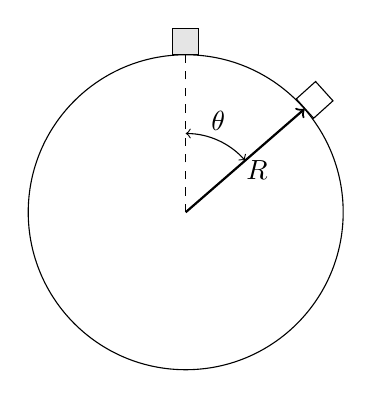
\begin{tikzpicture}
        %% globe
        \draw (0,0) circle (2cm);
        \draw[thick,->] (0,0) -- (41:2) node[anchor=north,pos=0.6] {$R$};
        \draw[dashed] (0,0) -- (90:2);
        \draw[<->] (0,1) arc(90:41:1) node[pos=0.5,anchor=south] {$\theta$};
        %% top block
        \node[anchor=south,draw,fill=white!90!black,minimum size=0.33cm] at (0,2) {};
        %% bottom block
        \node[anchor=south,draw,rotate=-48,minimum size=0.33cm] at (41:2) {};
    \end{tikzpicture}
    \end{center}
    At what angle $\theta$ does it slide off the surface of the globe?
    Assume the system is frictionless.
    \begin{multicols}{2}
    \begin{choices}
        \wrongchoice{$\theta = \ang{0}$}
        \wrongchoice{$\theta = \cos^{-1}\left(\dfrac{1}{3}\right)$}
      \correctchoice{$\theta = \cos^{-1}\left(\dfrac{2}{3}\right)$}
        \wrongchoice{$\theta = \ang{60}$}
        \wrongchoice{$\theta = \ang{90}$}
        %% added distractor ?
        %\wrongchoice{$\theta = \cos^{-1}\left(\dfrac{1}{2}\right)$}
    \end{choices}
    \end{multicols}
\end{question}
}

\element{aapt}{
\begin{questionmult}{olympiad-1996-q09}
    An object with mass $m$ and initial velocity $v$ is brought to rest by a constant force $F$ acting for a time $t$ and through a distance $d$.
    %Possible expressions for the magnitude of the force $F$ are:
    Which of these give(s) the correct expression for the magnitude of the force $F$?
    \begin{multicols}{3}
    \begin{choices}
        %% ANS is E
      \correctchoice{$\dfrac{mv^2}{2d}$}
      \correctchoice{$\dfrac{2md}{t^2}$}
      \correctchoice{$\dfrac{mv}{t}$}
    \end{choices}
    \end{multicols}
\end{questionmult}
}

\element{aapt}{
\begin{questionmult}{olympiad-1996-q10}
    A small sphere is moving at a constant speed in a vertical circle.
    %Below is a list of quantities that could be used to describe some aspect of the motion of the sphere.
    Which of these quantities will change as this sphere moves around the circle?
    \begin{choices}
        %% ANS is E
        \wrongchoice{kinetic energy}
      \correctchoice{potential energy}
      \correctchoice{momentum}
    \end{choices}
\end{questionmult}
}

\element{aapt}{
\begin{question}{olympiad-1996-q11}
    A roller coaster travels with speed $v_A$ at point $A$.
    Point $B$ is a height $H$ above point $A$.
    Assuming no frictional losses and no work done by a motor,
        what is the speed at point $B$?
    \begin{multicols}{2}
    \begin{choices}
      \correctchoice{$\sqrt{v_A^2 - 2gH}$}
        \wrongchoice{$v_A - \sqrt{2gH}$}
        \wrongchoice{$v_A - 2gH$}
        \wrongchoice{$v_A + \sqrt{2gH}$}
        \wrongchoice{$\sqrt{v_A^2 + 2gH}$}
    \end{choices}
    \end{multicols}
\end{question}
}

\element{aapt}{
\begin{question}{olympiad-1996-q12}
    Three air track cars are initially placed as shown in the accompanying figure.
    Car $A$ has mass $m$ and initial velocity $v$ to the right.
    Car $B$ with mass $m$ and car C with mass $4m$ are both initially at rest.
    \begin{center}
    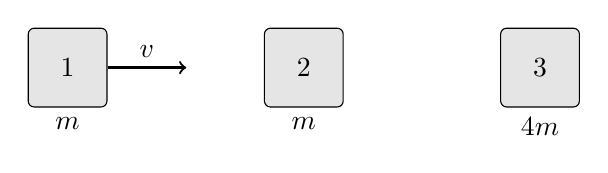
\begin{tikzpicture}
        %% Blocks
        \node[draw,minimum size=1cm,rounded corners=0.5ex,fill=white!90!black] (A) at (-3,0) {1};
        \node[draw,minimum size=1cm,rounded corners=0.5ex,fill=white!90!black] (B) at (+0,0) {2};
        \node[draw,minimum size=1cm,rounded corners=0.5ex,fill=white!90!black] (C) at (+3,0) {3};
        %% masses ??
        \node[anchor=north] at (A.south) {$m$};
        \node[anchor=north] at (B.south) {$m$};
        \node[anchor=north] at (C.south) {$4m$};
        %% Arrows
        \draw[thick,->] (A.east) -- ++(0:1cm) node[pos=0.5,anchor=south] {$v$};
    \end{tikzpicture}
    \end{center}
    Car $A$ collides elastically with car $B$,
        which in turn collides elastically with car $C$.
    After the collision, car $B$ is at rest.
    The final velocities of cars $A$ and $C$ are:
    \begin{choices}
      \correctchoice{Car $A$: $0.6v$ to the left; Car $C$: $0.4v$ to the right}
        \wrongchoice{Car $A$: $2.6v$ to the left; Car $C$: $0.4v$ to the right}
        \wrongchoice{Car $A$: at rest; Car $C$: $0.5v$ to the right}
        \wrongchoice{Car $A$: at rest; Car $C$: $0.25v$ to the right}
        \wrongchoice{Car $A$: at rest; Car $C$: $v$ to the right}
    \end{choices}
\end{question}
}

\element{aapt}{
\begin{question}{olympiad-1996-q13}
    A child with mass $m$ is standing at the edge of a playground merry-go-round with moment of inertia $I$,
        radius $R$, and initial angular velocity $\omega$.
    %% See figure to the right.
    \begin{center}
    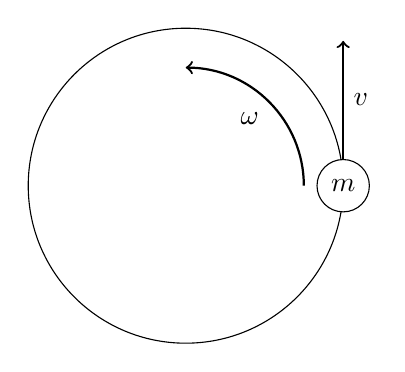
\begin{tikzpicture}
        \draw (0,0) circle (2cm);
        \node[draw,circle,fill=white] (M) at (2,0) {$m$};
        \draw[thick,->] (1.5,0) arc(0:90:1.5) node[pos=0.5,anchor=north east] {$\omega$};
        \draw[thick,->] (M.north) -- ++(90:1.5) node[pos=0.5,anchor=west] {$v$};
    \end{tikzpicture}
    \end{center}
    The child jumps off the edge of the merry-go-round with tangential velocity $v$ with respect to the ground.
    The new angular velocity of the merry-go-round is:
    %\begin{multicols}{2}
    \begin{choices}
        \wrongchoice{$\omega$}
        \wrongchoice{$\sqrt{\dfrac{I\omega^2 - mv^2}{I}}$}
        \wrongchoice{$\sqrt{\dfrac{\left(I+mR^2\right)\omega^2 - mv^2}{I}}$}
        \wrongchoice{$\dfrac{I\omega - mvR}{I}$}
      \correctchoice{$\dfrac{\left(I+mR^2\right)\omega^2 - mvR}{I}$}
    \end{choices}
    %\end{multicols}
\end{question}
}

\element{aapt}{
\begin{question}{olympiad-1996-q14}
    As shown in the figure below,
        a spool has outer radius $R$ and axle radius $r$.
    A string is wrapped around the axle of the spool and can be pulled in any of the directions labeled by I, II, or III.
    \begin{center}
    \begin{tikzpicture}
        %% ground
        \draw (-2,0) -- (4,0);
        \node[anchor=north,fill,pattern=north east lines,minimum width=6.0cm, minimum height=0.05cm] at (1,0) {};
        %% spool
        \draw[thick] (0,2) circle (1cm);
        \draw[thick] (0,2) circle (2cm);
        \draw[thick] (0,0) -- (0,2);
        %% r and R
        \draw[thick,->] (0,2)-- ++(180:1) node[pos=0.50,anchor=south] {$r$};
        \draw[thick,->] (0,2)-- ++(215:2) node[pos=0.75,anchor=south] {$R$};
        %% I, II, and III
        %% NOTE: TODO: double check these angles
        \draw[thick,->] (0,2) ++(300:1) -- ++(30:2.2) node[anchor=south west] {III};
        \draw[thick,->] (0,2) ++(315:1) -- ++(45:2.2) node[anchor=south west] {II};
        \draw[thick,->] (0,2) ++(350:1) -- ++(80:2.2) node[anchor=south west] {I};
    \end{tikzpicture}
    \end{center}
    The spool will slide to the right without rolling on the horizontal surface if it is pulled in direction(s):
    \begin{multicols}{2}
    \begin{choices}
        %% NOTE: questionmult
        \wrongchoice{I only}
      \correctchoice{II only}
        \wrongchoice{III only}
        \wrongchoice{I and II only}
        \wrongchoice{II and III only}
    \end{choices}
    \end{multicols}
\end{question}
}

\element{aapt}{
\begin{question}{olympiad-1996-q15}
    A uniform flag pole of length $L$ and mass $M$ is pivoted on the ground with a frictionless hinge.
    The flag pole makes an angle $\theta$ with the horizontal.
    The moment of inertia of the flag pole about one end is $\frac{1}{3} ML^2$.
    \begin{center}
    \begin{tikzpicture}
        %% ground
        \draw (-1,0) -- (5,0);
        \node[anchor=north,fill,pattern=north east lines,minimum width=6.0cm, minimum height=0.05cm] at (2,0) {};
        %% pivot and bar
        \draw (0,0) arc (270:-90:0.1cm);
        \draw[fill=white!90!black,rotate around={-45:(0,0.1)}] (-0.1,0.2) rectangle (0.1,5);
        \node[anchor=south west] at (45:5.0) {$P$};
        \draw[thick,<->] (-0.1,0.1) ++(135:0.5) -- ++(45:5) node[pos=0.5,anchor=center,fill=white,rotate=45] {$L$};
        %% angle
        \draw[<->] (1.5,0) arc(0:45:1.4) node[pos=0.5,anchor=west] {$\theta$};
    \end{tikzpicture}
    \end{center}
    If it starts falling from the position shown in the accompanying figure,
        the linear acceleration of the free end of the flag pole---labeled $P$---would be:
    \begin{multicols}{3}
    \begin{choices}
        \wrongchoice{$\dfrac{2g}{3}\cos\theta$}
        \wrongchoice{$\dfrac{2g}{3}$}
        \wrongchoice{$g$}
      \correctchoice{$\dfrac{3g}{2}\cos\theta$}
        \wrongchoice{$\dfrac{3g}{2}$}
    \end{choices}
    \end{multicols}
\end{question}
}

\element{aapt}{
\begin{question}{olympiad-1996-q16}
    The root mean square velocity of oxygen gas (atomic mass 16) is $v$ at room temperature.
    What is the root mean square velocity of helium (atomic mass 4) at the same temperature?
    \begin{multicols}{3}
    \begin{choices}
        \wrongchoice{$4 v$}
      \correctchoice{$2 v$}
        \wrongchoice{$v$}
        \wrongchoice{$\dfrac{v}{2}$}
        \wrongchoice{$\dfrac{v}{4}$}
    \end{choices}
    \end{multicols}
\end{question}
}

\element{aapt}{
\begin{question}{olympiad-1996-q17}
    Which of the accompanying $pV$ diagrams best represents an adiabatic process (process where no heat enters or leaves the system)?
    \begin{multicols}{2}
    \begin{choices}
        \AMCboxDimensions{down=-2.5em}
        \wrongchoice{
            \begin{tikzpicture}
                \begin{axis}[
                    axis y line=left,
                    axis x line=bottom,
                    axis line style={->},
                    xlabel={$V$},
                    xtick=\empty,
                    x label style={
                        at={(current axis.right of origin)},
                        anchor=west,
                    },
                    ylabel={$p$},
                    ytick=\empty,
                    y label style={
                        at={(current axis.above origin)},
                        anchor=east,
                        rotate=270,
                    },
                    xmin=0,xmax=10,
                    ymin=0,ymax=10,
                    width=0.95\columnwidth,
                ]
                \addplot[line width=1pt,domain=2:8]{6};
                \draw[thick,->] (axis cs:4,6) -- (axis cs:6,6);
                \end{axis}
            \end{tikzpicture}
        }
        \wrongchoice{
            \begin{tikzpicture}
                \begin{axis}[
                    axis y line=left,
                    axis x line=bottom,
                    axis line style={->},
                    xlabel={$V$},
                    xtick=\empty,
                    x label style={
                        at={(current axis.right of origin)},
                        anchor=west,
                    },
                    ylabel={$p$},
                    ytick=\empty,
                    y label style={
                        at={(current axis.above origin)},
                        anchor=east,
                        rotate=270,
                    },
                    xmin=0,xmax=10,
                    ymin=0,ymax=10,
                    width=0.95\columnwidth,
                ]
                \addplot[line width=1pt,no marks] plot coordinates { (1,1) (9,9) };
                \draw[thick,->] (axis cs:4,4) -- (axis cs:6,6);
                \end{axis}
            \end{tikzpicture}
        }
        %% ANS is C
        \correctchoice{
            \begin{tikzpicture}
                \begin{axis}[
                    axis y line=left,
                    axis x line=bottom,
                    axis line style={->},
                    xlabel={$V$},
                    xtick=\empty,
                    x label style={
                        at={(current axis.right of origin)},
                        anchor=west,
                    },
                    ylabel={$p$},
                    ytick=\empty,
                    y label style={
                        at={(current axis.above origin)},
                        anchor=east,
                        rotate=270,
                    },
                    xmin=0,xmax=10,
                    ymin=0,ymax=10,
                    width=0.95\columnwidth,
                ]
                \addplot[line width=1pt,domain=1:8]{ 22/x^(1.66) };
                \draw[thick,->] (axis cs:5,1.52) -- (axis cs:5.2,1.425);
                \end{axis}
            \end{tikzpicture}
        }
        \wrongchoice{
            \begin{tikzpicture}
                \begin{axis}[
                    axis y line=left,
                    axis x line=bottom,
                    axis line style={->},
                    xlabel={$V$},
                    xtick=\empty,
                    x label style={
                        at={(current axis.right of origin)},
                        anchor=west,
                    },
                    ylabel={$p$},
                    ytick=\empty,
                    y label style={
                        at={(current axis.above origin)},
                        anchor=east,
                        rotate=270,
                    },
                    xmin=0,xmax=10,
                    ymin=0,ymax=10,
                    width=0.95\columnwidth,
                ]
                \addplot[line width=1pt,domain=1:8]{ x^(1.66)/3.5 };
                \draw[thick,->] (axis cs:5,4.13) -- (axis cs:5.2,4.41);
                \end{axis}
            \end{tikzpicture}
        }
        \wrongchoice{
            \begin{tikzpicture}
                \begin{axis}[
                    axis y line=left,
                    axis x line=bottom,
                    axis line style={->},
                    xlabel={$V$},
                    xtick=\empty,
                    x label style={
                        at={(current axis.right of origin)},
                        anchor=west,
                    },
                    ylabel={$p$},
                    ytick=\empty,
                    y label style={
                        at={(current axis.above origin)},
                        anchor=east,
                        rotate=270,
                    },
                    xmin=0,xmax=10,
                    ymin=0,ymax=10,
                    width=0.95\columnwidth,
                ]
                \addplot[line width=1pt,no marks] plot coordinates { (5,1) (5,9) };
                \draw[thick,->] (axis cs:5,4) -- (axis cs:5,6);
                \end{axis}
            \end{tikzpicture}
        }
    \end{choices}
    \end{multicols}
\end{question}
}

\element{aapt}{
\begin{question}{olympiad-1996-q18}
    String $A$ and String $B$ have the same mass and length.
    String $A$ is under tension $T$ and string $B$ is under tension $2T$.
    The speed of waves in $B$ is \rule[-0.1pt]{4em}{0.1pt} times the speed of waves in $A$.
    \begin{multicols}{3}
    \begin{choices}
        \wrongchoice{0.50}
        \wrongchoice{0.71}
        \wrongchoice{1.00}
      \correctchoice{1.4}
        \wrongchoice{2.0}
    \end{choices}
    \end{multicols}
\end{question}
}

\element{aapt}{
\begin{question}{olympiad-1996-q19}
    On a day when the velocity of sound in air is $v$,
        a whistle moves with velocity $u$ toward a stationary wall. 
    \begin{center}
    \begin{tikzpicture}
        %% Floor and Wall
        \draw (-7,0) -- (0,0);
        \node[anchor=north,fill,pattern=north east lines,minimum width=7.0cm, minimum height=0.05cm] at (-3.5,0) {};
        \draw[line width=1.5pt] (0,-0.25) -- (0,3);
        %% cart
        \node[draw,anchor=south,minimum width=1.5cm,minimum height=0.5cm] (A) at (-5,0.4) {};
        %% wheels
        \draw (A.south east) ++(180:0.3cm) arc(-270:90:0.2);
        \draw (A.south west) ++(0:0.3cm) arc(-270:90:0.2);
        %% velocity
        \draw[thick,->] (A.east) -- ++(0:1.5) node[pos=0.5,anchor=south] {$u$};
        %% whistle
        \draw[thick] (A.north) ++(0:0.25) ++ (90:0.25) --++(180:0.5) --++(90:1) --++(0:0.5) --++(270:0.2) --++(180:0.2) -- ++(-60:0.4) -- cycle;
        \draw (A.north) -- ++(90:0.25);
    \end{tikzpicture}
    \end{center}
    The whistle emits sound with frequency $f$. 
    What frequency of reflected sound will be heard by an observer traveling along with the whistle?
    \begin{multicols}{3}
    \begin{choices}
        \wrongchoice{$f \dfrac{v-u}{v+u}$}
        \wrongchoice{$f \dfrac{v}{v+u}$}
        \wrongchoice{$f$}
        \wrongchoice{$f \dfrac{v-u}{v-u}$}
      \correctchoice{$f \dfrac{v+u}{v-u}$}
    \end{choices}
    \end{multicols}
\end{question}
}

\element{aapt}{
\begin{question}{olympiad-1996-q20}
    You are given two lenses, a converging lens with focal length \SI{+10}{\centi\meter} and a diverging lens with focal length \SI{-20}{\centi\meter}.
    Which of the following would produce a real image that is larger than the object?
    \begin{choices}
        \wrongchoice{Placing the object \SI{5}{\centi\meter} from the converging lens.}
      \correctchoice{Placing the object \SI{15}{\centi\meter} from the converging lens.}
        \wrongchoice{Placing the object \SI{25}{\centi\meter} from the converging lens.}
        \wrongchoice{Placing the object \SI{15}{\centi\meter} from the diverging lens.}
        \wrongchoice{Placing the object \SI{25}{\centi\meter} from the diverging lens.}
    \end{choices}
\end{question}
}

\element{aapt}{
\begin{question}{olympiad-1996-q21}
    Two mirrors, labeled $LM$ for left mirror and $RM$ for right mirror in the accompanying figure,
        are parallel to each other and \SI{3.0}{\meter} apart. 
    \begin{center}
    \begin{tikzpicture}
        %% Left and right mirror
        \draw[very thick] (-4,-1) -- (-4,3) node[anchor=south] {$LM$};
        \draw[very thick] (+2,-1) -- (+2,3) node[anchor=south] {$RM$};
        %% Arrows
        \draw[<->] (-3.95,-0.5) -- (-0.05,-0.5) node[pos=0.5,anchor=north] {\SI{2.0}{\meter}};
        \draw[<->] (+1.95,-0.5) -- (+0.05,-0.5) node[pos=0.5,anchor=north] {\SI{1.0}{\meter}};
        %%% Man
        \begin{scope}[anchor=south,scale=2.0]
            \draw[thick] (0,0.25) -- (0,0.75);
            %% Legs
            \draw[thick] (0,0.25) -- (-0.25,0);
            \draw[thick] (0,0.25) -- (+0.25,0);
            %% Arms
            \draw[thick] (0,0.50) -- (-0.25,0.55);
            \draw[thick] (0,0.50) -- (+0.25,0.55);
            %% Head
            \draw[fill=white!90!black] (0,0.80) circle (0.15cm);
        \end{scope}
    \end{tikzpicture}
    \end{center}
    A person standing \SI{1.0}{\meter} from the right mirror ($RM$) looks into this mirror and sees a series of images. 
    How far from the person is the second closest image seen in the right mirror ($RM$)?
    \begin{multicols}{3}
    \begin{choices}
        \wrongchoice{\SI{2.0}{\meter}}
        \wrongchoice{\SI{4.0}{\meter}}
      \correctchoice{\SI{6.0}{\meter}}
        \wrongchoice{\SI{8.0}{\meter}}
        \wrongchoice{\SI{10.0}{\meter}}
    \end{choices}
    \end{multicols}
\end{question}
}

\element{aapt}{
\begin{question}{olympiad-1996-q22}
    A thin film of thickness $t$ and index of refraction 1.33 coats a glass with index of refraction 1.50. 
    \begin{center}
    \begin{tikzpicture}
        \draw (-3,1) -- (3,1);
        \draw (-3,0) -- (3,0);
        %% thickness
        \draw[<->] (-2.5,1) -- (-2.5,0) node[pos=0.5,anchor=center,fill=white] {$t$};
        %% index of refraction
        \node[anchor=east] at (3,1.5) {$n=1.00$};
        \node[anchor=east] at (3,0.5) {$n=1.33$};
        \node[anchor=east] at (3,-0.5) {$n=1.50$};
        %% Path
        \draw[very thick] (-0.5,1) -- ++(100:1.5);
        \draw[very thick,->] (-0.5,1) -- ++(80:1.5);
        \draw[very thick,->] (-0.5,1) -- ++(-80:1.003) -- ++(80:2.5);
    \end{tikzpicture}
    \end{center}
    What is the least thickness $t$ that will strongly reflect light with wavelength \SI{600}{\nano\meter}? 
    Hint: Light undergoes a \ang{180} phase shift when it is reflected off a material with a higher index of refraction.
    \begin{multicols}{3}
    \begin{choices}
      \correctchoice{\SI{225}{\nano\meter}}
        \wrongchoice{\SI{300}{\nano\meter}}
        \wrongchoice{\SI{400}{\nano\meter}}
        \wrongchoice{\SI{450}{\nano\meter}}
        \wrongchoice{\SI{600}{\nano\meter}}
    \end{choices}
    \end{multicols}
\end{question}
}

\element{aapt}{
\begin{question}{olympiad-1996-q23}
    The accompanying figure shows two concentric spherical shells isolated from each other. 
    The smaller shell has radius $b$ and net charge $+Q$.
    The larger shell has radius $2b$ and an equal net charge $+Q$. 
    \begin{center}
    \begin{tikzpicture}
        %% small sphere
        \draw (0,0) circle (1cm);
        \draw[thick,->] (0,0) -- (45:1) node[pos=0.5,anchor=south,rotate=45] {$b$};
        \node[anchor=west] at (0:1) {$+Q$};
        %% large sphere
        \draw (0,0) circle (2cm);
        \draw[thick,->] (0,0) -- (315:2) node[pos=0.75,anchor=south,rotate=-45] {$2b$};
        \node[anchor= south west] at (45:2) {$+Q$};
    \end{tikzpicture}
    \end{center}
    If $R$ is the distance from the common center,
        the highest electric field magnitude $E$ occurs:
    \begin{choices}
        \wrongchoice{only at $R=0$, where $E$ is infinite.}
        \wrongchoice{anywhere $R<b$, where $E$ is constant}
      \correctchoice{immediately outside the smaller ($R=b$) shell.}
        \wrongchoice{immediately outside the larger ($R=2b$) shell.}
        \wrongchoice{far away from the shells; $E$ increases with distance.}
    \end{choices}
\end{question}
}

\element{aapt}{
\begin{question}{olympiad-1996-q24}
    An infinite conducting plate of thickness \SI{0.0200}{\meter} is surrounded by a uniform field $E=\SI{400}{\volt\per\meter}$ directed left to right. 
    %See the figure to the right. 
    \begin{center}
    \begin{tikzpicture}
        %% conducting plate
        \draw[white,fill=white!90!black] (-1,0) rectangle (1,3);
        %% boundaries
        \draw[dotted] (-4,0) -- (-4,3);
        \draw[dotted] (-1,0) -- (-1,3);
        \draw[dotted] (+1,0) -- (+1,3);
        \draw[dotted] (+3,0) -- (+3,3);
        % E field
        \draw[thick,->] (-3,2) -- (-2,2) node[pos=0.5,anchor=south] {$E$};
        \draw[thick,->] (+1.5,2) -- (+2.5,2) node[pos=0.5,anchor=south] {$E$};
        % Voltage
        \draw[thick,<->] (-4,1) -- (-1,1)   
            node[pos=0.0,anchor=south west] {$V_3$}
            node[pos=0.5,anchor=north] {\SI{0.030}{\meter}}
            node[pos=1.0,anchor=south east] {$V_2$};
        \draw[thick,<->] (+1,1) -- (+3,1)   
            node[pos=0.0,anchor=south west] {$V_1$}
            node[pos=0.5,anchor=north] {\SI{0.020}{\meter}}
            node[pos=1.0,anchor=south east] {$V_0$};
        \draw[thick,<->] (-1,1) -- (+1,1)   
            node[pos=0.5,anchor=north] {\SI{0.020}{\meter}};
    \end{tikzpicture}
    \end{center}
    Let the potential $V_0=0$ a distance \SI{0.0200}{\meter} to the right of the plate. 
    What is $V_3$, the potential \SI{0.0300}{\meter} to the left of the plate?
    \begin{multicols}{3}
    \begin{choices}
        \wrongchoice{\SI{-28}{\volt}}
        \wrongchoice{\SI{-20}{\volt}}
        \wrongchoice{\SI{+12}{\volt}}
      \correctchoice{\SI{+20}{\volt}}
        \wrongchoice{\SI{+28}{\volt}}
    \end{choices}
    \end{multicols}
\end{question}
}

\element{aapt}{
\begin{question}{olympiad-1996-q25}
    A sphere of radius $a$ has uniform charge density $\rho$.
    A spherical cavity of radius $c$ is formed in the sphere. 
    The cavity is centered a distance $b$ ($b>c$) from the center of the sphere. 
    \begin{center}
    \begin{tikzpicture}
        %% spherical cavity
        \draw[fill=white!90!black] (0,0) circle (2cm);
        \draw[fill=white] (1,0) circle (0.5cm);
        %% radius
        \draw[thick,->] (0,0) -- (135:2) node[pos=0.5,anchor=south west] {$a$};
        \draw[thick,->] (0,0) -- (1,0) node[pos=0.25,anchor=north] {$b$};
        \draw[thick,->] (1,0) -- ++(45:0.5) node[pos=0.25,anchor=north west] {$c$};
    \end{tikzpicture}
    \end{center}
    What is the magnitude of the electric field at the center of the cavity?
    \begin{multicols}{2}
    \begin{choices}
      \correctchoice{$\dfrac{\rho b}{3\varepsilon_0}$}
        \wrongchoice{$\dfrac{\rho a^3}{3\varepsilon_0 b^2}$}
        \wrongchoice{$\dfrac{\rho \left(a^3-c^3\right)}{3\varepsilon_0 b^2}$}
        \wrongchoice{$\dfrac{\rho}{3\varepsilon_0} \left(b-\dfrac{c^3}{2b^2}\right)$}
        \wrongchoice{$\dfrac{\rho}{3\varepsilon_0} \left(b-\dfrac{c^3}{b^2}\right)$}
        %\wrongchoice{$\dfrac{\rho \left(b-\dfrac{c^3}{2b^2}\right)}{3\varepsilon_0}$}
        %\wrongchoice{$\dfrac{\rho \left(b-\dfrac{c^3}{b^2}\right)}{3\varepsilon_0}$}
    \end{choices}
    \end{multicols}
\end{question}
}

\element{aapt}{
\begin{question}{olympiad-1996-q26}
    As shown in the diagram below, two fixed charges,
    \begin{center}
    \begin{tikzpicture}
        %% charges
        \draw[fill=white!90!black] (-3,0) circle (5pt) node[anchor=north,yshift=-5pt] {$q_1$};
        \draw[fill=white!90!black] (+3,0) circle (5pt) node[anchor=north,yshift=-5pt] {$q_2$};
        %% distance
        \draw[dashed,<->] (-2.8cm,0) -- (+2.8cm,0) node[pos=0.5,anchor=center,fill=white] {\SI{0.200}{\meter}};
    \end{tikzpicture}
    \end{center}
    $q_1 = \SI{+1.00}{\micro\coulomb}$ and $q_2=\SI{-4.00}{\micro\coulomb}$, are \SI{0.200}{\meter} apart. 
    Where is the total field zero?
    \begin{choices}
        \wrongchoice{\SI{0.40}{\meter} to the right of $q_1$}
        \wrongchoice{\SI{0.13}{\meter} to the right of $q_1$}
        \wrongchoice{\SI{0.1}{\meter} to the right of $q_1$}
        \wrongchoice{\SI{0.067}{\meter} to the left of $q_1$}
      \correctchoice{\SI{0.20}{\meter} to the left of $q_1$}
    \end{choices}
\end{question}
}

\element{aapt}{
\begin{question}{olympiad-1996-q27}
    The switch, $S$, is closed in the circuit shown below.
    \begin{center}
    \ctikzset{bipoles/length=1.00cm}
    \begin{circuitikz}
        \draw (0,0) to [battery,l=\SI{6.0}{\volt}] (0,2) to [cspst,l=$S$] (0,4)
                    to [R,l=\SI{100}{\ohm}] (2,4) to (4,4) to [C,l=\SI{10.0}{\micro\farad}] (4,0) to (0,0);
        \draw (2,4) to [R,l=\SI{200}{\ohm}] (2,0);
    \end{circuitikz}
    \end{center}
    What is the charge on the capacitor when it is fully charged?
    \begin{multicols}{3}
    \begin{choices}
        \wrongchoice{\SI{5.0}{\micro\coulomb}}
        \wrongchoice{\SI{10}{\micro\coulomb}}
        \wrongchoice{\SI{20}{\micro\coulomb}}
      \correctchoice{\SI{40}{\micro\coulomb}}
        \wrongchoice{\SI{60}{\micro\coulomb}}
    \end{choices}
    \end{multicols}
\end{question}
}

\element{aapt}{
\begin{question}{olympiad-1996-q28}
    Two identical resistors with resistance $R$ are connected in the two circuits drawn below. 
    \begin{center}
    \ctikzset{bipoles/length=1.00cm}
    \begin{circuitikz}
        %% NOTE: Place label inside circuit??
        \begin{scope}[yshift=+1.5cm]
            \draw (0,0) to [battery,l=\SI{12}{\volt}] (0,2) to [R,l=$R$] (4,2) to (4,0) to [R,l_=$R$] (0,0);
            \node[anchor=north] at (-1.5,2) {I};
            %\node[anchor=north] at (0.5,1) {I};
        \end{scope}
        \begin{scope}[yshift=-1.5cm]
            \draw (0,0) to [battery,l=\SI{12}{\volt}] (0,2) to (2,2) to [R,l=$R$] (2,0);
            \draw (2,2) to (4,2) to [R,l=$R$] (4,0) to (0,0);
            \node[anchor=north] at (-1.5,2) {II};
        \end{scope}
    \end{circuitikz}
    \end{center}
    The battery in both circuits is a \SI{12}{\volt} battery. 
    Which statement is correct?
    \begin{choices}
        \wrongchoice{More current will flow through each R in circuit I than in circuit II.}
      \correctchoice{More total power will be delivered by the battery in circuit II than in circuit I.}
        \wrongchoice{The potential drop across each R will be greater in circuit I than in circuit II.}
        \wrongchoice{The equivalent resistance will be greater in circuit II than in circuit I.}
        \wrongchoice{The power dissipated in each R will be greater in circuit I than in circuit II.}
    \end{choices}
\end{question}
}

\element{aapt}{
\begin{question}{olympiad-1996-q29}
    The resistors---$R_1$, $R_2$, and $R_3$---have been adjusted so that the current in the ammeter (labeled $A$ in the accompanying circuit diagram) is zero. 
    \begin{center}
    \ctikzset{bipoles/length=0.75cm}
    \begin{circuitikz}
        \draw (0,0) to [battery,l=$V$] (4,0) to (4,2) to [R,l=$R_2$] (2,2) to [R,l=$R_1$] (0,2);
        \draw (4,2) to (4,6) to [R,l=$R$] (2,6) to [R,l=$R_3$] (0,6) to (0,0);
        \draw (2,6) to [ammeter,l=$A$] (2,2);
    \end{circuitikz}
    \end{center}
    What is $R$?
    \begin{multicols}{3}
    \begin{choices}
        \wrongchoice{$R_2$}
        \wrongchoice{$R_3$}
        \wrongchoice{$\dfrac{R_1 R_2}{R_3}$}
        \wrongchoice{$\dfrac{R_1 R_3}{R_2}$}
      \correctchoice{$\dfrac{R_2 R_3}{R_1}$}
    \end{choices}
    \end{multicols}
\end{question}
}

\element{aapt}{
\begin{question}{olympiad-1996-q30}
    A long cylindrical conducting wire---shown in cross section below---carries a conventional current out of the page. 
    \begin{center}
    \begin{tikzpicture}
        %% cylindrical a and R
        \draw (0,0) circle (2cm);
        \draw (0,0) circle (1cm);
        %% radius a and R
        \draw[thick,->] (0,0) -- ++(45:2) node[pos=0.75,anchor=south east] {$a$};
        \draw[thick,->] (0,0) -- ++(135:1) node[pos=0.5,anchor=north east] {$R$};
    \end{tikzpicture}
    \end{center}
    The wire has uniform current density $J$ and radius $a$. 
    What is the magnetic field inside the wire,
        a distance $R$ ($R<a$) from the wire's center?
    \begin{choices}
        \wrongchoice{$\dfrac{\mu_0 J a}{2}$ clockwise}
        \wrongchoice{$\dfrac{\mu_0 J a^2}{2R}$ clockwise}
      \correctchoice{$\dfrac{\mu_0 J R}{2}$ counterclockwise}
        \wrongchoice{$\dfrac{\mu_0 J a^2}{2R}$ counterclockwise}
        \wrongchoice{$\dfrac{\mu_0 J a}{2}$ counterclockwise}
    \end{choices}
\end{question}
}


%% PhysicsOlympiad 1997 Screening Exam
%%----------------------------------------
\element{aapt}{
\begin{question}{olympiad-1997-q01}
    Starting from rest at time $t=0$,
        a car moves in a straight line with an acceleration given by the accompanying graph.
    \begin{center}
    \begin{tikzpicture}
        \begin{axis}[
            axis y line=left,
            axis x line=bottom,
            axis line style={->},
            xlabel={time},
            x unit=\si{\second},
            xtick={0,2,4,6},
            minor x tick num=1,
            ylabel={acceleration},
            y unit=\si{\meter\per\second\squared},
            ytick={0,2,4,6},
            minor y tick num=1,
            grid=major,
            xmin=0,xmax=6.1,
            ymin=0,ymax=6.2,
            width=0.8\columnwidth,
            height=0.5\columnwidth,
        ]
        \addplot[line width=1.5pt,no marks] plot coordinates { (0,5) (5,0) (6,0) };
        \end{axis}
    \end{tikzpicture}
    \end{center}
    What is the speed of the car at $t=\SI{3}{\second}$?
    \begin{multicols}{3}
    \begin{choices}
        \wrongchoice{\SI{1.0}{\meter\per\second}}
        \wrongchoice{\SI{2.0}{\meter\per\second}}
        \wrongchoice{\SI{6.0}{\meter\per\second}}
      \correctchoice{\SI{10.5}{\meter\per\second}}
        \wrongchoice{\SI{12.5}{\meter\per\second}}
    \end{choices}
    \end{multicols}
\end{question}
}

\element{aapt}{
\begin{question}{olympiad-1997-q02}
    A flare is dropped from a plane flying over level ground at a velocity of \SI{70}{\meter\per\second} in the horizontal direction.
    At the instant the flare is released, the plane begins to accelerate horizontally at \SI{0.75}{\meter\per\second\squared}.
    The flare takes \SI{4.0}{\second} to reach the ground.
    Assume air resistance is negligible.
    Relative to a spot directly under the flare at release,
        the flare lands directly on the spot.
    \begin{choices}
        \wrongchoice{directly on the spot}
        \wrongchoice{\SI{6.0}{\meter} in front of the spot.}
        \wrongchoice{\SI{274}{\meter} in front of the spot.}
      \correctchoice{\SI{280}{\meter} in front of the spot.}
        \wrongchoice{\SI{286}{\meter} in front of the spot.}
    \end{choices}
\end{question}
}

\element{aapt}{
\begin{question}{olympiad-1997-q03}
    %% NOTE: make independent
    As seen by the pilot of the plane (in question \#2) and measured relative to a spot directly under the plane when the flare lands,
        the flare lands:
    \begin{choices}
        \wrongchoice{\SI{286}{\meter} behind the plane.}
      \correctchoice{\SI{6.0}{\meter} behind the plane.}
        \wrongchoice{directly under the plane.}
        \wrongchoice{\SI{12}{\meter} in front of the plane.}
        \wrongchoice{\SI{274}{\meter} in front of the plane}
    \end{choices}
\end{question}
}

\element{aapt}{
\begin{question}{olympiad-1997-q04}
    A force $F$ is used to hold a block of mass $m$ on an incline as shown in the diagram.
    \begin{center}
    \begin{tikzpicture}
        %% incline
        \draw[thick] (0,0) -- (30:6);
        \draw[thick,dashed] (0,0) -- (0:5.196);
        \draw[<->] (1.5,0) arc (0:30:1.5) node[pos=0.5,anchor=west] {$\theta$};
        %% block
        \node[draw,anchor=south,minimum size=1cm,rotate=30,fill=white!90!black] (A) at (30:4) {};
        %% force
        \draw[very thick,<-] (A.north) -- ++(120:1) node[pos=0.5,anchor=west] {$F$};
    \end{tikzpicture}
    \end{center}
    The plane makes an angle of $\theta$ with the horizontal and $F$ is perpendicular to the plane.
    The coefficient of friction between the plane and the block is $\mu$.
    What is the minimum force, $F$, necessary to keep the block at rest?
    \begin{multicols}{2}
    \begin{choices}
        \wrongchoice{$\mu mg$}
        \wrongchoice{$mg \cos\theta$}
        \wrongchoice{$mg \sin\theta$}
        \wrongchoice{$\dfrac{mg}{\mu} \sin\theta$}
      \correctchoice{$\dfrac{mg}{\mu} \left(\sin\theta-\mu\cos\theta\right)$}
    \end{choices}
    \end{multicols}
\end{question}
}

\element{aapt}{
\begin{question}{olympiad-1997-q05}
    You hold a rubber ball in your hand.
    The Newton's third law companion force to the force of gravity on the ball is the force exerted by the:
    \begin{choices}
      \correctchoice{ball on the Earth.}
        \wrongchoice{ball on the hand.}
        \wrongchoice{hand on the ball.}
        \wrongchoice{Earth on the ball.}
        \wrongchoice{Earth on your hand.}
    \end{choices}
\end{question}
}

\element{aapt}{
\begin{question}{olympiad-1997-q06}
    A ball of mass $m$ is fastened to a string.
    The ball swings in a vertical circle of radius $R$ with the other end of the string held fixed.
    Neglecting air resistance,
        the difference between the string's tension at the bottom of the circle and at the top of the circle is:
    \begin{multicols}{3}
    \begin{choices}
        \wrongchoice{$mg$}
        \wrongchoice{$2 mg$}
        \wrongchoice{$4 mg$}
      \correctchoice{$6 mg$}
        \wrongchoice{$8 mg$}
    \end{choices}
    \end{multicols}
\end{question}
}

\element{aapt}{
\begin{question}{olympiad-1997-q07}
    Three air track cars, shown in the accompanying figure,
        all have the same mass $m$.
    \begin{center}
    \begin{tikzpicture}
        %% Blocks
        \node[draw,minimum size=1cm,rounded corners=0.5ex,fill=white!90!black] (A) at (-3,0) {1};
        \node[draw,minimum size=1cm,rounded corners=0.5ex,fill=white!90!black] (B) at (+0,0) {2};
        \node[draw,minimum size=1cm,rounded corners=0.5ex,fill=white!90!black] (C) at (+3,0) {3};
        %% masses ??
        \node[anchor=north] at (A.south) {$m$};
        \node[anchor=north] at (B.south) {$m$};
        \node[anchor=north] at (C.south) {$m$};
        %% Arrows
        \draw[thick,->] (A.east) -- ++(0:1cm) node[pos=0.5,anchor=south] {$v$};
    \end{tikzpicture}
    \end{center}
    Cars 2 and 3 are initially at rest.
    Car 1 is moving to the right with speed $v$.
    Car 1 collides with car 2 and sticks to it.
    The 1-2 combination collides elastically with car 3.
    Which of the following is most nearly the final speed of car 3?
    \begin{multicols}{3}
    \begin{choices}
        \wrongchoice{$0.17 v$}
        \wrongchoice{$0.50 v$}
      \correctchoice{$0.67 v$}
        \wrongchoice{$0.80 v$}
        \wrongchoice{$1.00 v$}
    \end{choices}
    \end{multicols}
\end{question}
}

\element{aapt}{
\begin{question}{olympiad-1997-q08}
    A point object of mass $2m$ is attached to one end of a rigid rod of negligible mass and length $L$.
    The rod is initially at rest but free to rotate about a fixed axis perpendicular to the rod and passing through its other end.
    \begin{center}
    \begin{tikzpicture}[font=\footnotesize]
        \begin{scope}[xshift=-1.25cm]
            %% point mass
            \node[draw,circle] (A) at (-2,-2) {$m$};
            \draw[thick,->] (A.east) -- ++(0:1cm) node[pos=0.5,anchor=south] {$v$};
            %% rod
            \draw[fill] (-2pt,2cm) rectangle (2pt,-2cm);
            \node[anchor=east] at (-2pt,0) {$L$};
            %% 2m
            \node[draw,circle,fill=white] (B) at (0,-2) {$2m$};
        \end{scope}
        \begin{scope}[xshift=+0.25cm,rotate around={30:(0,2)}]
            %% point mass
            \node[draw,circle] (C) at (-0.5,-2) {$m$};
            %% rod
            \draw[fill] (-2pt,2cm) rectangle (2pt,-2cm);
            \node[anchor=east] at (-5pt,0) {$L$};
            %% 2m
            \node[draw,circle,fill=white] (D) at (0,-2) {$2m$};
            \draw[thick,->] (D.north east) -- ++(0:1cm) node[pos=0.5,anchor=south] {$v_t$};
        \end{scope}
    \end{tikzpicture}
    \end{center}
    A second point object with mass $m$ and initial speed $v$ collides and sticks to the $2m$ object.
    What is the tangential speed $v_t$ of the object immediately after the collision?
    \begin{multicols}{3}
    \begin{choices}
      \correctchoice{$\dfrac{v}{3}$}
        \wrongchoice{$\dfrac{v}{2}$}
        \wrongchoice{$\dfrac{v}{\sqrt{3}}$}
        \wrongchoice{$\dfrac{v}{\sqrt{2}}$}
        \wrongchoice{$\dfrac{2v}{\sqrt{3}}$}
    \end{choices}
    \end{multicols}
\end{question}
}

\element{aapt}{
\begin{question}{olympiad-1997-q09}
    Two artificial satellites I and II have circular orbits of radii $R$ and $2R$,
        respectively, about the same planet.
    The orbital velocity of satellite I is $v$.
    What is the orbital velocity of satellite II?
    \begin{multicols}{3}
    \begin{choices}
        \wrongchoice{$\dfrac{v}{2}$}
      \correctchoice{$\dfrac{v}{\sqrt{2}}$}
        \wrongchoice{$v$}
        \wrongchoice{$\sqrt{2}v$}
        \wrongchoice{$2v$}
    \end{choices}
    \end{multicols}
\end{question}
}

\element{aapt}{
\begin{question}{olympiad-1997-q10}
    The gravitational acceleration on the surface of the moon is \SI{1.6}{\meter\per\second\squared}.
    The radius of the moon is \SI{1.7e6}{\meter}.
    The period of a satellite placed in a low circular orbit about the moon is most nearly:
    \begin{multicols}{2}
    \begin{choices}
        \wrongchoice{\SI{1.0e3}{\second}}
      \correctchoice{\SI{6.5e3}{\second}}
        \wrongchoice{\SI{1.1e6}{\second}}
        \wrongchoice{\SI{5.0e6}{\second}}
        \wrongchoice{\SI{7.1e12}{\second}}
    \end{choices}
    \end{multicols}
\end{question}
}

\element{aapt}{
\begin{question}{olympiad-1997-q11}
    A uniform ladder of length $L$ rests against a smooth frictionless wall.
    \begin{center}
    \begin{tikzpicture}
        %% Wall and Floor
        \draw (0,0) -- (3,0);
        \node[anchor=north,fill,pattern=north east lines,minimum width=3.0cm, minimum height=0.05cm] at (1.5,0) {};
        \draw (0,0) -- (0,5);
        \node[anchor=east,fill,pattern=north east lines,minimum width=0.05cm, minimum height=5.2cm] at (0,2.4) {};
        %% ladder
        \draw[line width=2pt] (0,4) -- (2,0);
        %% angle
        \draw[<->] (1,0) arc(180:116:1) node[pos=0.5,anchor=east] {$\theta$};
    \end{tikzpicture}
    \end{center}
    The floor is rough and the coefficient of static friction between the floor and ladder is $\mu$.
    When the ladder is positioned at angle $\theta$,
        as shown in the accompanying diagram,
        it is just about to slip.
    What is $\theta$?
    \begin{multicols}{2}
    \begin{choices}
        \wrongchoice{$\theta = \dfrac{\mu}{L}$}
        \wrongchoice{$\tan\theta = 2\mu$}
      \correctchoice{$\tan\theta = \dfrac{1}{2\mu}$}
        \wrongchoice{$\sin\theta = \dfrac{1}{\mu}$}
        \wrongchoice{$\cos\theta = \mu$}
    \end{choices}
    \end{multicols}
\end{question}
}

\element{aapt}{
\begin{questionmult}{olympiad-1997-q12}
    Three objects, all of mass $M$,
        are released simultaneously from the top of an inclined plane of height $H$.
    The objects are described as follows:
    %% NOTE: TODO: finish this?
    Assume the cylinders roll down the plane without slipping and the cube slides down the plane without friction.
    Which object(s) reach(es) the bottom of the plane first?
    \begin{choices}
      \correctchoice{a cube of side $R$.}
        \wrongchoice{a solid cylinder of radius $R$}
        \wrongchoice{a hollow cylinder of radius $R$}
        %% I %% II %% III %% I & II %% II & III
    \end{choices}
\end{questionmult}
}

\element{aapt}{
\begin{question}{olympiad-1997-q13}
    A massless rod of length $2R$ can rotate about a vertical axis through its center as shown in the diagram.
    \begin{center}
    \begin{tikzpicture}
        \begin{scope}[yshift=+0.5cm]
            \draw (-3,0) -- (3,0);
            \draw[fill=white!90!black] (-3,0) circle (5pt);
            \draw[fill=white!90!black] (+3,0) circle (5pt);
            \draw[thick,->] (0,0.5) -- (3,0.5) node[pos=0.5,anchor=south] {$R$};
            \draw[dashed] (0,0.75) -- (0,-0.5);
        \end{scope}
        \begin{scope}[yshift=-0.5cm]
            \draw (-3,0) -- (3,0);
            \draw[fill=white!90!black] (-1.5,0) circle (5pt);
            \draw[fill=white!90!black] (+1.5,0) circle (5pt);
            \draw[thick,->] (0,-0.5) -- (1.5,-0.5) node[pos=0.5,anchor=north] {$R/2$};
            \draw[dashed] (0,0.5) -- (0,-0.75);
        \end{scope}
    \end{tikzpicture}
    \end{center}
    The system rotates at an angular velocity $\omega$ when the two masses $m$ are a distance $R$ from the axis.
    The masses are simultaneously pulled to a distance of $R/2$ from the axis by a force directed along the rod.
    What is the new angular velocity of the system?
    \begin{multicols}{3}
    \begin{choices}
        \wrongchoice{$\dfrac{\omega}{4}$}
        \wrongchoice{$\dfrac{\omega}{2}$}
        \wrongchoice{$\omega$}
        \wrongchoice{$2\omega$}
      \correctchoice{$4\omega$}
    \end{choices}
    \end{multicols}
\end{question}
}

\element{aapt}{
\begin{question}{olympiad-1997-q14}
    A meter stick moves with a velocity of $0.60 c$ relative to an observer.
    The observer measures the length of the meter stick to be $L$.
    Which of the following statements is always true?
    \begin{multicols}{2}
    \begin{choices}
        \wrongchoice{$L=\SI{0.60}{\meter}$}
        \wrongchoice{$L=\SI{0.80}{\meter}$}
      \correctchoice{$\SI{0.80}{\meter\squared} L^2 \SI{1.00}{\meter}$}
        %% NOTE: TODO: finish this??
        \wrongchoice{$L=\SI{1.00}{\meter}$}
        \wrongchoice{$L 3 \SI{1.00}{\meter}$}
    \end{choices}
    \end{multicols}
\end{question}
}

\element{aapt}{
\begin{question}{olympiad-1997-q15}
    A glowing ember (hot piece of charcoal) radiates power $P$ in watts at an absolute temperature $T$.
    When the temperature of the ember has decreased to $T/2$,
        the power it radiates is most nearly:
    \begin{multicols}{3}
    \begin{choices}
        \wrongchoice{$P$}
        \wrongchoice{$\dfrac{P}{2}$}
        \wrongchoice{$\dfrac{P}{4}$}
        \wrongchoice{$\dfrac{P}{8}$}
      \correctchoice{$\dfrac{P}{16}$}
    \end{choices}
    \end{multicols}
\end{question}
}

\newcommand{\aaptOlympiadNinetySevenQSixteen}{
\begin{tikzpicture}
    \begin{semilogyaxis}[
        clip=false,
        axis y line=left,
        axis x line=bottom,
        axis line style={->},
        xlabel={$V$},
        xtick=\empty,
        %x label style={
        %    at={(current axis.right of origin)},
        %    anchor=west,
        %},
        ylabel={$p$},
        ytick=\empty,
        y label style={
            at={(current axis.above origin)},
            anchor=east,
            rotate=270,
        },
        xmin=0,xmax=10,
        ymin=0.5,ymax=16,
        width=0.8\columnwidth,
        height=0.5\columnwidth,
    ]
    \node[anchor=south] at (axis cs:2,8) {1};
    \node[anchor=west] at (axis cs:8,2) {2};
    \node[anchor=west] at (axis cs:8,0.8) {3};
    \addplot[line width=1pt,domain=2:8]{ 25/x^(1.66) };
    \draw[thick,->]  (axis cs:5.1,1.69) -- (axis cs:5,1.74);
    \addplot[line width=1pt,domain=2:8]{ 16/x };
    \draw[thick,->] (axis cs:5,3.2) -- (axis cs:5.1,3.17);
    \addplot[line width=1pt,domain=2:8] plot coordinates { (8,0.8) (8,2) };
    \draw[thick,->] (axis cs:8,1.1) -- (axis cs:8,0.9);
    \end{semilogyaxis}
\end{tikzpicture}
}

\element{aapt}{
\begin{question}{olympiad-1997-q16}
    Three processes compose a thermodynamic cycle shown in the accompanying pV diagram of an ideal gas.
    \begin{center}
        \aaptOlympiadNinetySevenQSixteen
    \end{center}
    Process $1\to 2$ takes place at constant temperature (\SI{300}{\kelvin}).
    During this process \SI{60}{\joule} of heat enters the system.
    Process $2\to 3$ takes place at constant volume.
    During this process \SI{40}{\joule} of heat leaves the system.
    Process $3\to 1$ is adiabatic.
    $T_3$ is \SI{275}{\kelvin}.
    %% start question
    What is the change in internal energy of the system during process $3\to 1$?
    \begin{multicols}{3}
    \begin{choices}
        \wrongchoice{\SI{-40}{\joule}}
        \wrongchoice{\SI{-20}{\joule}}
        \wrongchoice{zero}
        \wrongchoice{\SI{+20}{\joule}}
      \correctchoice{\SI{+40}{\joule}}
    \end{choices}
    \end{multicols}
\end{question}
}

\element{aapt}{
\begin{question}{olympiad-1997-q17}
    Three processes compose a thermodynamic cycle shown in the accompanying pV diagram of an ideal gas.
    \begin{center}
        \aaptOlympiadNinetySevenQSixteen
    \end{center}
    Process $1\to 2$ takes place at constant temperature (\SI{300}{\kelvin}).
    During this process \SI{60}{\joule} of heat enters the system.
    Process $2\to 3$ takes place at constant volume.
    During this process \SI{40}{\joule} of heat leaves the system.
    Process $3\to 1$ is adiabatic.
    $T_3$ is \SI{275}{\kelvin}.
    %% start question
    %What is the change in entropy of the system described in Question \#16 during the process $3\to 1$?
    What is the change in entropy of the system during the process $3\to 1$?
    \begin{multicols}{3}
    \begin{choices}
        \wrongchoice{\SI{+5.0}{\kelvin\per\joule}}
        \wrongchoice{\SI{+0.20}{\joule\per\kelvin}}
      \correctchoice{zero}
        \wrongchoice{\SI{-1.6}{\joule\per\kelvin}}
        \wrongchoice{\SI{-6.9}{\kelvin\per\joule}}
    \end{choices}
    \end{multicols}
\end{question}
}

\element{aapt}{
\begin{question}{olympiad-1997-q18}
    A wave is described by the equation: $y(x,t) = 0.030 \sin\left(5\pi x + 4\pi t\right)$ where $x$ and $y$ are in meters and $t$ is in seconds.
    The $+x$ direction is to the right.
    What is the velocity of the wave?
    \begin{choices}
      \correctchoice{\SI{0.80}{\meter\per\second} to the left}
        \wrongchoice{\SI{1.25}{\meter\per\second} to the left}
        \wrongchoice{\SI[parse-numbers=false]{0.12\pi}{\meter\per\second} to the right}
        \wrongchoice{\SI{0.80}{\meter\per\second} to the right}
        \wrongchoice{\SI{1.25}{\meter\per\second} to the right}
    \end{choices}
\end{question}
}

\element{aapt}{
\begin{question}{olympiad-1997-q19}
    Two sources, in phase and a distance $d$ apart,
        each emit a wave of wavelength $\lambda$.
    %See accompanying figure.
    \begin{center}
    \begin{tikzpicture}
        %% Two sources
        \draw[fill] (0,+1) circle (2pt);
        \draw[fill] (0,-1) circle (2pt);
        \draw[<->] (-0.3,-1) -- (-0.3,+1) node[pos=0.5,anchor=center,fill=white] {$d$};
        %% point P
        \draw[fill] (6,2) circle (1pt) node[anchor=south] {$P$};
        \draw (0,+1) -- (6,2) node[pos=0.1,anchor=south,rotate=14] {$L_2$};
        \draw (0,-1) -- (6,2) node[pos=0.1,anchor=south,rotate=37] {$L_1$};
        %% distance x
        \draw[<->] (6,0) -- (6,1.95) node[pos=0.5,anchor=center,fill=white] {$x$};
        \draw[dashed] (-0.1,0) -- (6.1,0);
        \draw[dashed] (0,0) -- (6,2);
        \draw[<->] (1.5,0) arc (0:18.4:1.5) node[pos=0.5,anchor=west] {$\theta$};
    \end{tikzpicture}
    \end{center}
    Which of the choices for the path difference $\Delta L = L_1 - L_2$ will \emph{always} produce destructive interference at point $P$?
    \begin{multicols}{3}
    \begin{choices}
        \wrongchoice{$d\sin\theta$}
        \wrongchoice{$\dfrac{x}{L_1}$}
        \wrongchoice{$d\dfrac{x}{L_2}$}
      \correctchoice{$\dfrac{\lambda}{2}$}
        \wrongchoice{$2\lambda$}
    \end{choices}
    \end{multicols}
\end{question}
}

\element{aapt}{
\begin{question}{olympiad-1997-q20}
    You are given two lenses,
        a converging lens with focal length \SI{+10}{\centi\meter} and a diverging lens with focal length \SI{-20}{\centi\meter}.
    Which of the following would produce a virtual image that is larger than the object?
    \begin{choices}
      \correctchoice{Placing the object \SI{5}{\centi\meter} from the converging lens.}
        \wrongchoice{Placing the object \SI{15}{\centi\meter} from the converging lens.}
        \wrongchoice{Placing the object \SI{25}{\centi\meter} from the converging lens.}
        \wrongchoice{Placing the object \SI{15}{\centi\meter} from the diverging lens.}
        \wrongchoice{Placing the object \SI{25}{\centi\meter} from the diverging lens.}
    \end{choices}
\end{question}
}

\element{aapt}{
\begin{question}{olympiad-1997-q21}
    You are given two identical plano-convex lenses,
        one of which is shown on the right.
    %% NOTE: TODO: remove to the right ??
    \begin{center}
    \begin{tikzpicture}
        %% NOTE: TODO: draw tikz
        \begin{scope}[xshift=-1.5cm]
            \draw (0,0) arc(180:175:26.6);
            \draw (0,0) arc(180:195:26.6);
            %\draw (0,-1) -- (0,+1);
            \node[anchor=north] at (0,-2) {Planoconvex};
        \end{scope}
        \begin{scope}[xshift=+1.5cm]
            \draw (0,0) arc (180:175:26.6); 
            \draw (0,0) arc (180:195:26.6); 
            \node at (0,-1) {Double Convex};
        \end{scope}
    \end{tikzpicture}
    \end{center}
    When you place an object \SI{20}{\centi\meter} to the left of a single plano-convex lens,
        the image appears \SI{40}{\centi\meter} to the right of the lens.
    You then arrange the two plano-convex lenses back to back to form a double convex lens.
    If the object is \SI{20}{\centi\meter} to the left of this new lens,
        what is the approximate location of the image?
    \begin{choices}
        \wrongchoice{\SI{6.7}{\centi\meter} to the right of the lens.}
      \correctchoice{\SI{10}{\centi\meter} to the right of the lens.}
        \wrongchoice{\SI{20}{\centi\meter} to the right of the lens.}
        \wrongchoice{\SI{80}{\centi\meter} to the right of the lens.}
        \wrongchoice{\SI{80}{\centi\meter} to the left of the lens.}
    \end{choices}
\end{question}
}

\element{aapt}{
\begin{question}{olympiad-1997-q22}
    Positive charge $Q$ is uniformly distributed over a ring of radius a that lies in the $y$-$z$ plane as shown in the diagram.
    The ring is centered at the origin.
    \begin{center}
    \begin{tikzpicture}
        %% Coordinates
        \draw[thick,-latex] (+3,0) -- (-3,0) node[anchor=north] {$z$};
        \draw[thick,-latex] (0,-3) -- (0,+3) node[anchor=west] {$y$};
        \draw[thick,-latex] (-2,1.15) -- (3.46,-2) node[anchor=north] {$x$};
        %% Ring
        \draw[line width=2pt] (0,0) circle (2cm);
        %\draw[thick,->] (0,0) -- (45:2cm) node[pos=0.5,anchor=south] {$a$};
        \node[anchor=south east] at (120:2) {$Q$};
    \end{tikzpicture}
    \end{center}
    Which of the following graphs best represents the value of the electric field $E$ as a function of $x$,
        the distance along the positive $x$ axis?
    \begin{multicols}{2}
    \begin{choices}
        \AMCboxDimensions{down=-2.5em}
        %% NOTE: ANS is D
        \wrongchoice{
            %% NOTE: TODO: FINISH this
            \begin{tikzpicture}
                \begin{axis}[
                    axis y line=left,
                    axis x line=bottom,
                    axis line style={->},
                    xlabel={$x$},
                    xtick=\empty,
                    ylabel={$E$},
                    ytick=\empty,
                    xmin=0,xmax=10,
                    ymin=0,ymax=10,
                    width=0.95\columnwidth,
                ]
                \addplot[line width=1pt,domain=0:10]{6};
                \end{axis}
            \end{tikzpicture}
        }
    \end{choices}
    \end{multicols}
\end{question}
}

\element{aapt}{
\begin{question}{olympiad-1997-q23}
    Four point charges are placed at the corners of a square with diagonal $2a$ as shown in the diagram.
    \begin{center}
    \begin{tikzpicture}
        %% coordinates
        \draw[thick,->] (0,0) -- (2,0) node[anchor=north] {$x$};
        \draw[thick,->] (0,0) -- (0,2) node[anchor=west] {$y$};
        %% Charges
        \draw[fill=white!90!black] (-2,-2) circle (5pt) node [anchor=west,xshift=5pt] {$-2q$};
        \draw[fill=white!90!black] (-2,+2) circle (5pt) node [anchor=west,xshift=5pt] {$+3q$};
        \draw[fill=white!90!black] (+2,+2) circle (5pt) node [anchor=east,xshift=-5pt] {$-q$};
        \draw[fill=white!90!black] (+2,-2) circle (5pt) node [anchor=east,xshift=-5pt] {$+3q$};
        %% 2a
        \draw[thick,dashed,<->] (-1.88,1.88) -- (1.88,-1.88) node[pos=0.25,anchor=north,rotate=-45] {$2a$};
    \end{tikzpicture}
    \end{center}
    What is the total electric field at the center of the square?
    \begin{choices}
        \wrongchoice{$\dfrac{kq}{a^2}$ at an angle \ang{45} above the $+x$ axis.}
      \correctchoice{$\dfrac{kq}{a^2}$ at an angle \ang{45} below the $-x$ axis.}
        \wrongchoice{$\dfrac{3 kq}{a^2}$ at an angle \ang{45} above the $-x$ axis.}
        \wrongchoice{$\dfrac{3 kq}{a^2}$ at an angle \ang{45} below the $+x$ axis.}
        \wrongchoice{$\dfrac{9 kq}{a^2}$ at an angle \ang{45} above the $+x$ axis.}
    \end{choices}
\end{question}
}

\newcommand{\olympiadNinetySevenQTwentyFour}{
\begin{tikzpicture}
    %% spherical shell
    \draw[fill=white!90!black] (0,0) circle (2cm);
    \draw[fill=white] (0,0) circle (1.5cm);
    %% radius
    \draw[-latex] (0,0) -- (90:1.5) node[pos=0.5,anchor=west] {$a$};
    \draw[-latex] (0,0) -- (315:2.0) node[pos=0.5,anchor=south,rotate=-45] {$b$};
    %% -q and Q
    \node[anchor=east] (0,0) {$Q$};
    \node[anchor=center] at (225:1.88) {$-q$};
\end{tikzpicture}
}

\element{aapt}{
\begin{question}{olympiad-1997-q24}
    %Both questions 24 and 25 refer to the system shown in the diagram.
    A spherical shell with an inner surface of radius $a$ and an outer surface of radius $b$ is made of conducting material.
    A point charge $+Q$ is placed at the center of the spherical shell and a total charge $-q$ is placed on the shell.
    \begin{center}
        \olympiadNinetySevenQTwentyFour
    \end{center}
    %% start question
    How is the charge $-q$ distributed after it has reached equilibrium?
    \begin{choices}
        \wrongchoice{Zero charge on the inner surface, $-q$ on the outer surface.}
        \wrongchoice{$-Q$ on the inner surface, $-q$ on the outer surface.}
      \correctchoice{$-Q$ on the inner surface, $-q+Q$ on the outer surface.}
        \wrongchoice{$+Q$ on the inner surface, $-q-Q$ on the outer surface.}
        \wrongchoice{The charge $-q$ is spread uniformly between the inner and outer surface.}
    \end{choices}
\end{question}
}

\element{aapt}{
\begin{question}{olympiad-1997-q25}
    %Both questions 24 and 25 refer to the system shown in the diagram.
    A spherical shell with an inner surface of radius $a$ and an outer surface of radius $b$ is made of conducting material.
    A point charge $+Q$ is placed at the center of the spherical shell and a total charge $-q$ is placed on the shell.
    \begin{center}
        \olympiadNinetySevenQTwentyFour
    \end{center}
    %% start question
    Assume that the electrostatic potential is zero at an infinite distance from the spherical shell.
    What is the electrostatic potential at a distance $R$ from the center of the shell,
        where $b^3 R^3 a$?
    \begin{multicols}{3}
    \begin{choices}
        \wrongchoice{zero}
        \wrongchoice{$k\dfrac{Q}{a}$}
        \wrongchoice{$k\dfrac{Q}{R}$}
        \wrongchoice{$k\dfrac{Q-q}{R}$}
      \correctchoice{$k\dfrac{Q-q}{b}$}
    \end{choices}
    \end{multicols}
\end{question}
}

\newcommand{\olympiadNinetySevenQTwentySix}{
\begin{circuitikz}
    %% This is duplicate graphic from before, uses L_1 instead of B_1
    %% NOTE: TODO: draw tikz
\end{circuitikz}
}

\element{aapt}{
\begin{question}{olympiad-1997-q26}
    %% Use the circuit below to answer questions 26 and 27.
    $B_1$ , $B_2$, $B_3$, and $B_4$ are identical light bulbs.
    There are six voltmeters connected to the circuit as shown.
    \begin{center}
        \olympiadNinetySevenQTwentySix
    \end{center}
    All voltmeters are connected so that they display positive voltages.
    Assume that the voltmeters do not effect the circuit.
    %% start question
    If $B_2$ were to burn out,
        opening the circuit, which voltmeter(s) would read zero volts?
    \begin{choices}
      \correctchoice{none would read zero.}
        \wrongchoice{only $V_2$}
        \wrongchoice{only $V_3$ and $V_4$}
        \wrongchoice{only $V_3$, $V_4$ , and $V_5$}
        \wrongchoice{they would all read zero}
    \end{choices}
\end{question}
}

\element{aapt}{
\begin{question}{olympiad-1997-q27}
    %% Use the circuit below to answer questions 26 and 27.
    $B_1$ , $B_2$, $B_3$, and $B_4$ are identical light bulbs.
    There are six voltmeters connected to the circuit as shown.
    \begin{center}
        \olympiadNinetySevenQTwentySix
    \end{center}
    All voltmeters are connected so that they display positive voltages.
    Assume that the voltmeters do not effect the circuit.
    %% start question
    If $B_2$ were to burn out, opening the circuit,
        what would happen to the reading of V 1 ?
    Let $V$ be its original reading when all bulbs are functioning and let $V^{\prime}$ be its reading when $B_2$ is burnt out.
    \begin{multicols}{2}
    \begin{choices}
        \wrongchoice{$V^{\prime} > 2V$}
        \wrongchoice{$2V > V^{\prime} > V$}
        \wrongchoice{$V^{\prime} = V$}
      \correctchoice{$V > V^{\prime} > \dfrac{V}{2}$}
        \wrongchoice{$\dfrac{V}{2} > V^{\prime}$}
    \end{choices}
    \end{multicols}
\end{question}
}

\element{aapt}{
\begin{question}{olympiad-1997-q28}
    A particle with positive charge $q$ and mass $m$ travels along a path perpendicular to a magnetic field.
    The particle moves in a circle of radius $R$ with frequency $f$.
    What is the magnitude of the magnetic field?
    \begin{multicols}{3}
    \begin{choices}
        \wrongchoice{$\dfrac{mf}{q}$}
      \correctchoice{$\dfrac{2\pi fm}{q}$}
        \wrongchoice{$\dfrac{m}{2\pi fq}$}
        \wrongchoice{$\dfrac{mc}{qR}$}
        \wrongchoice{$\dfrac{\mu qf}{2\pi R}$}
    \end{choices}
    \end{multicols}
\end{question}
}

\element{aapt}{
\begin{question}{olympiad-1997-q29}
    %% NOTE: to the right
    Two wires, each carrying a current $i$, are shown in the diagram to the right.
    Both wires extend in a straight line for a very long distance on both the right and the left.
    One wire contains a semi-circular loop of radius a centered on point $X$.
    \begin{center}
    \begin{tikzpicture}
        %% NOTE: TODO: draw tikz
        %% top wire
        \draw (-3,1) -- (3,1);
        \draw[thick,->] (-0.5,1) -- (0.5,1) node[pos=0.5,anchor=south] {$i$};
        %% bottom wire
        \draw (-3,0) -- (-1,0) arc(180:360:1cm) -- (3,0);
        \draw[thick,->] (3,0) -- (2,0) node[pos=0.5,anchor=north] {$i$};
        %% Point X
        \draw[fill] (0,0) circle (1.5pt) node[anchor=south east] {$X$};
        \draw[thick,->] (0,0) -- (315:1cm) node[pos=0.5,anchor=south,rotate=-45] {$a$};
        %% width a
        \draw[thick,<->] (-1.5,0.05) -- (-1.5,0.95) node[pos=0.5,anchor=center,fill=white] {$a$};
    \end{tikzpicture}
    \end{center}
    What is the correct expression for the magnetic field at point $X$?
    HINT: The magnitude of the magnetic field at the center of a circular current loop of radius $R$ is $\mu_0 i/(2R)$.
    \begin{choices}
        %% NOTE: Align options with \makebox[ ]{ }
        \wrongchoice{\makebox[8em][l]{$\dfrac{\mu_0 i}{4a} + \dfrac{\mu_0 i}{2\pi a}$} out of the page}
        %% NOTE: TODO: this could  be reduced
        \wrongchoice{\makebox[8em][l]{$\dfrac{\mu_0 i}{2a} - \dfrac{\mu_0 i}{2\pi a} + \dfrac{\mu_0 i}{2\pi a}$} out of the page}
      \correctchoice{\makebox[8em][l]{$\dfrac{\mu_0 i}{4a} + \dfrac{\mu_0 i}{2\pi a}$} into the page}
        %% NOTE: TODO: this could  be reduced
        \wrongchoice{\makebox[8em][l]{$\dfrac{\mu_0 i}{4a} + \dfrac{\mu_0 i}{2\pi a} + \dfrac{\mu_0 i}{2\pi a}$} into the page}
        \wrongchoice{\makebox[8em][l]{$\dfrac{\mu_0 i}{2a} - \dfrac{\mu_0 i}{2\pi a}$} into the page}
    \end{choices}
\end{question}
}

\element{aapt}{
\begin{questionmult}{olympiad-1997-q30}
    You are given a bar magnet and a looped coil of wire.
    \begin{center}
    \begin{tikzpicture}
        %% Loops
        \foreach \i in {1mm,3mm,5mm,7mm} {
            \draw (\i,0) circle (0.2cm and 1.5cm);
        }
        %% magnet
        \node[draw,fill=white!90!black,minimum width=1.5cm,minimum height=0.5cm,anchor=center] (M) at (-3,0) {};
        \draw[thick,->] (M.east) ++(0,+0.15) to[out=0,in=220]  ++(30:1.5);
        \draw[thick,->] (M.east) ++(0,+0.07) to[out=0,in=200]  ++(15:1.5);
        \draw[thick,->] (M.east) to[out=0,in=180]  ++(0:1.5);
        \draw[thick,->] (M.east) ++(0,-0.07) to[out=0,in=160]  ++(-15:1.5);
        \draw[thick,->] (M.east) ++(0,-0.15) to[out=0,in=140]  ++(-30:1.5);
    \end{tikzpicture}
    \end{center}
    Which of the following would induce an emf in the coil?
    \begin{choices}
      \correctchoice{Moving the magnet toward the coil.}
      \correctchoice{Moving the coil away from the magnet.}
      \correctchoice{Turning the coil about a vertical axis.}
        %% A. I only B. II only C. I & II D. I & III E. I, II, III
    \end{choices}
\end{questionmult}
}


%% PhysicsOlympiad 1998 Screening Exam
%%----------------------------------------
\element{aapt}{
\begin{question}{olympiad-1998-q01}
    The graph below is a plot of position versus time.
    \begin{center}
    \begin{tikzpicture}
        \begin{axis}[
            axis y line=left,
            axis x line=bottom,
            axis line style={->},
            xlabel={time},
            xtick=\empty,
            ylabel={position},
            ytick=\empty,
            xmin=0,xmax=11,
            ymin=0,ymax=11,
            width=0.8\columnwidth,
            height=0.5\columnwidth,
        ]
        %% TODO: NOTE: draw function
        \addplot[mark=\empty,thick,smooth] plot coordinates { (0,3) (5,9) (8,1) (10,6) };
        %% guesswork
        \draw[fill] (axis cs:1,4.5) circle (1.5pt) node[anchor=north] {$A$};
        \draw[fill] (axis cs:3,7.3) circle (1.5pt) node[anchor=north] {$B$};
        \draw[fill] (axis cs:5,9) circle (1.5pt) node[anchor=north] {$C$};
        \draw[fill] (axis cs:6.7,5) circle (1.5pt) node[anchor=west] {$D$};
        \draw[fill] (axis cs:8,1) circle (1.5pt) node[anchor=south] {$E$};
        \end{axis}
    \end{tikzpicture}
    \end{center}
    For which labeled region is the velocity positive and the acceleration negative?
    \begin{multicols}{3}
    \begin{choices}[o]
        \wrongchoice{$A$}
        \wrongchoice{$B$}
        \wrongchoice{$C$}
        \wrongchoice{$D$}
      \correctchoice{$E$}
    \end{choices}
    \end{multicols}
\end{question}
}

\element{aapt}{
\begin{question}{olympiad-1998-q02}
    A child left her home and started walking at a constant velocity.
    After a time she stopped for a while and then continued on with a velocity greater than she originally had.
    All of a sudden she turned around and walked very quickly back home.
    Which of the following graphs best represents the distance versus time graph for her walk?
    \begin{multicols}{2}
    \begin{choices}
        %% NOTE: pgfplots??
        %% NOTE: ANS is B
        \wrongchoice{
            \begin{tikzpicture}
            \end{tikzpicture}
        }
    \end{choices}
    \end{multicols}
\end{question}
}

\element{aapt}{
\begin{question}{olympiad-1998-q03}
    In a rescue attempt, a hovering helicopter drops a life preserver to a swimmer being swept downstream by a river current of constant velocity $v$.
    The helicopter is at a height of \SI{9.8}{\meter}.
    The swimmer is \SI{6.0}{\meter} upstream from a point directly under the helicopter when the life preserver is released.
    It lands \SI{2.0}{\meter} in front of the swimmer.
    How fast is the current flowing?
    Neglect air resistance.
    \begin{multicols}{3}
    \begin{choices}
        \wrongchoice{\SI{13.7}{\meter\per\second}}
        \wrongchoice{\SI{9.8}{\meter\per\second}}
        \wrongchoice{\SI{6.3}{\meter\per\second}}
      \correctchoice{\SI{2.8}{\meter\per\second}}
        \wrongchoice{\SI{2.4}{\meter\per\second}}
    \end{choices}
    \end{multicols}
\end{question}
}

\element{aapt}{
\begin{question}{olympiad-1998-q04}
    A child tosses a ball directly upward.
    Its total time in the air is $T$.
    Its maximum height is $H$.
    What is its height after it has been in the air a time $T/4$?
    Neglect air resistance.
    \begin{multicols}{3}
    \begin{choices}
        \wrongchoice{$\dfrac{1}{4} H$}
        \wrongchoice{$\dfrac{1}{3} H$}
        \wrongchoice{$\dfrac{1}{2} H$}
        \wrongchoice{$\dfrac{2}{3} H$}
      \correctchoice{$\dfrac{3}{4} H$}
    \end{choices}
    \end{multicols}
\end{question}
}

\element{aapt}{
\begin{questionmult}{olympiad-1998-q05}
    A whiffle ball is tossed straight up, reaches a highest point, and falls back down.
    Air resistance is not negligible.
    Which of the following statements are true?
    \begin{choices}
      \correctchoice{The ball’s speed is zero at the highest point.}
        \wrongchoice{The ball’s acceleration is zero at the highest point.}
        \wrongchoice{The ball takes a longer time to travel up to the highest point than to fall back down.}
        %% A. I only B. II only C. I & II only D. I & III only E. I, II, & III
    \end{choices}
\end{questionmult}
}

\element{aapt}{
\begin{question}{olympiad-1998-q06}
    A pendulum is attached to the ceiling of an elevator car.
    When the car is parked, the pendulum exhibits a period of \SI{1.00}{\second}.
    The car now begins to travel upward with an upward acceleration of \SI{2.3}{\meter\per\second\squared}.
    During this part of the motion,
        what will be the approximate period of the pendulum?
    \begin{multicols}{3}
    \begin{choices}
        \wrongchoice{\SI{0.80}{\second}}
      \correctchoice{\SI{0.90}{\second}}
        \wrongchoice{\SI{1.00}{\second}}
        \wrongchoice{\SI{1.10}{\second}}
        \wrongchoice{\SI{1.20}{\second}}
    \end{choices}
    \end{multicols}
\end{question}
}

\element{aapt}{
\begin{question}{olympiad-1998-q07}
    Two identical blocks of weight $W$ are placed one on top of the other as shown below.
    \begin{center}
    \begin{tikzpicture}
        %% Ground
        \draw (0,0) -- (-6,0);
        \node[anchor=north,fill,pattern=north east lines,minimum width=6cm, minimum height=0.05cm] at (-3,0) {};
        %% Wall
        \draw (0,0) -- (0,3);
        \node[anchor=west,fill,pattern=north east lines,minimum width=0.1cm, minimum height=3.2cm] at (0,+1.4) {};
        %% block
        \node[fill=white!90!black,rounded corners=1ex,minimum width=2cm,minimum height=1cm,draw,anchor=south] (B) at (-3,0) {$m$};
        \node[fill=white!90!black,rounded corners=1ex,minimum width=2cm,minimum height=1cm,draw,anchor=south] (T) at (B.north) {$m$};
        %% force
        \draw[very thick,->] (B.west) -- ++(180:1.5) node[pos=0.5,anchor=south] {$F$};
        \draw[very thick] (T.east) -- ++(0:2);
    \end{tikzpicture}
    \end{center}
    The upper block is tied to the wall.
    The lower block is pulled to the right with a force $F$.
    The coefficient of static friction between all surfaces in contact is $\mu$.
    What is the largest force $F$ that can be exerted before the lower block starts to slip?
    \begin{multicols}{3}
    \begin{choices}
        \wrongchoice{$\mu W$}
        \wrongchoice{$\dfrac{3}{2} \mu W$}
        \wrongchoice{$2 \mu W$}
        \wrongchoice{$\dfrac{5}{2} \mu W$}
      \correctchoice{$3 \mu W$}
    \end{choices}
    \end{multicols}
\end{question}
}

\element{aapt}{
\begin{question}{olympiad-1998-q08}
    An object placed on an equal arm balance requires \SI{12}{\kilo\gram} to balance it.
    When placed on a spring scale, the scale reads \SI{120}{\newton}.
    Everything (balance, scale, set of masses, and the object) is now transported to the moon where the gravitational force is one-sixth that on Earth.
    The new readings of the balance and the spring scale (respectively) are:
    \begin{multicols}{2}
    \begin{choices}
      \correctchoice{\SI{12}{\kilo\gram}, \SI{20}{\newton}}
        \wrongchoice{\SI{12}{\kilo\gram}, \SI{120}{\newton}}
        \wrongchoice{\SI{12}{\kilo\gram}, \SI{720}{\newton}}
        \wrongchoice{\SI{2}{\kilo\gram}, \SI{20}{\newton}}
        \wrongchoice{\SI{2}{\kilo\gram}, \SI{120}{\newton}}
    \end{choices}
    \end{multicols}
\end{question}
}

\element{aapt}{
\begin{question}{olympiad-1998-q09}
    A large spool of rope lies on the ground in the diagram below.
    \begin{center}
    \begin{tikzpicture}
        %% Ground
        \draw (-2,0) -- (+4,0);
        \node[anchor=north,fill,pattern=north east lines,minimum width=6cm, minimum height=0.05cm] at (1,0) {};
        %% Spool
        \draw[thick] (0,2) circle (2cm);
        %% Rope
        \draw[thick,->] (0,4) -- ++(0:4) node[anchor=north east] {$X$};
    \end{tikzpicture}
    \end{center}
    The end, labeled $X$, is pulled a distance $S$ in the horizontal direction.
    The spool rolls without slipping.
    The distance the spool’s center of mass moves is:
    \begin{multicols}{3}
    \begin{choices}
        \wrongchoice{$2S$}
        \wrongchoice{$S$}
      \correctchoice{$\dfrac{S}{2}$}
        \wrongchoice{$\dfrac{S}{3}$}
        \wrongchoice{$\dfrac{S}{4}$}
    \end{choices}
    \end{multicols}
\end{question}
}

\element{aapt}{
\begin{question}{olympiad-1998-q10}
    Air track car $Z$ of mass \SI{1.5}{\kilo\gram} approaches and collides with air track car $R$ of mass \SI{2.0}{\kilo\gram}.
    %See the accompanying diagram.
    \begin{center}
    \begin{tikzpicture}
        %% Track
        \draw[thick] (-4,0) -- (4,0);
        %% Carts
        \node[draw,minimum width=1.8cm,minimum height=0.9cm,fill=white,anchor=base,yshift=2mm] (Z) at (-2.5,0) {$Z$};
        \node[draw,minimum width=1.8cm,minimum height=0.9cm,fill=white,anchor=base,yshift=2mm] (R) at (+2.5,0) {$R$};
        %% Spring
        \draw[decoration={aspect=0.2,segment length=1.5mm,amplitude=2mm,coil},decorate] (R.west) -- ++(180:1);
        %% Vector
        \draw[very thick,-latex] (Z.south west) ++(270:0.5) -- ++(0:1.8);
    \end{tikzpicture}
    \end{center}
    Car $R$ has a spring attached to it and is initially at rest.
    When the separation between the cars has reached a minimum, then:
    \begin{choices}
        \wrongchoice{car $R$ is still at rest.}
        \wrongchoice{car $Z$ has come to rest.}
        \wrongchoice{both cars have the same kinetic energy.}
        \wrongchoice{both cars have the same momentum.}
      \correctchoice{the kinetic energy of the system has reached a minimum.}
    \end{choices}
\end{question}
}

\element{aapt}{
\begin{question}{olympiad-1998-q11}
    Two ice skaters, a \SI{200}{\pound} man and a \SI{120}{\pound} woman,
        are initially hugging on a frictionless level ice surface.
    Ten seconds after they push off from each other,
        they are \SI{8.0}{\meter} apart.
    How far has the woman moved in that time?
    \begin{multicols}{3}
    \begin{choices}
        \wrongchoice{\SI{8.0}{\meter}}
        \wrongchoice{\SI{6.5}{\meter}}
      \correctchoice{\SI{5.0}{\meter}}
        \wrongchoice{\SI{4.0}{\meter}}
        \wrongchoice{\SI{3.0}{\meter}}
    \end{choices}
    \end{multicols}
\end{question}
}

\element{aapt}{
\begin{questionmult}{olympiad-1998-q12}
    %% NOTE: to the right
    The diagram to the right shows the velocity-time graph for two masses $R$ and $S$ that collided elastically.
    \begin{center}
    %% NOTE: TODO: pgfplots
    \begin{tikzpicture}
        \begin{axis}[
            axis y line=left,
            axis x line=bottom,
            axis line style={->},
            xlabel={time},
            x unit=\si{\second},
            xtick={0,1,2,3,4},
            minor x tick num=1,
            ylabel={velocity},
            y unit=\si{\meter\per\second},
            ytick={0.0,0.4,0.8,1.2},
            minor y tick num=1,
            grid=major,
            xmin=0,xmax=4.05,
            ymin=0,ymax=1.205,
            width=0.8\columnwidth,
            height=0.5\columnwidth,
        ]
        \addplot[line width=1pt,no marks] plot coordinates { (0,0.8) (1,0.8) (3,0.2) (4,0.2) };
        \node[anchor=south] at (axis cs:0.5,0.8) {$R$};
        \addplot[line width=1pt,no marks] plot coordinates { (0,0) (1,0) (3,1.0) (4,1.0) };
        \node[anchor=north] at (axis cs:3.5,1.0) {$S$};
        \end{axis}
    \end{tikzpicture}
    \end{center}
    Which of the following statements is true?
    \begin{choices}
      \correctchoice{$R$ and $S$ moved in the same direction after the collision.}
      \correctchoice{The velocities of $R$ and $S$ were equal at the mid-time of the collision.}
        \wrongchoice{The mass of $S$ was greater than the mass of $R$.}
        %% A. I only B. II only C. I & II only D. II & III only E. I, II & III
    \end{choices}
\end{questionmult}
}

\element{aapt}{
\begin{question}{olympiad-1998-q13}
    %%  NOTE: reword
    %% Questions 13 and 14 refer to the motion of two blocks along a frictionless level track.
    Two blocks are in motion along a frictionless level track.
    Block \#1 (mass $m_1$) is initially moving with speed $v_0$.
    It collides with and sticks to an initially stationary block (\#2) of mass $m_2 = 9 m_1$.
    %% start question
    What is the speed of the two blocks after the collision?
    \begin{multicols}{3}
    \begin{choices}
        \wrongchoice{$v_0$}
        \wrongchoice{$\dfrac{9}{10} v_0$}
        \wrongchoice{$\dfrac{8}{9} v_0$}
        \wrongchoice{$\dfrac{1}{9} v_0$}
      \correctchoice{$\dfrac{1}{10} v_0$}
    \end{choices}
    \end{multicols}
\end{question}
}

\element{aapt}{
\begin{question}{olympiad-1998-q14}
    %%  NOTE: reword
    %% Questions 13 and 14 refer to the motion of two blocks along a frictionless level track.
    Two blocks are in motion along a frictionless level track.
    Block \#1 (mass $m_1$) is initially moving with speed $v_0$.
    It collides with and sticks to an initially stationary block (\#2) of mass $m_2 = 9 m_1$.
    %% start question
    What fraction of the initial kinetic energy of the system is converted to other forms (heat, sound, \ldots) as a result of the collision?
    \begin{multicols}{3}
    \begin{choices}
        \wrongchoice{\SI{1}{\percent}}
        \wrongchoice{\SI{10}{\percent}}
        \wrongchoice{\SI{50}{\percent}}
      \correctchoice{\SI{90}{\percent}}
        \wrongchoice{\SI{99}{\percent}}
    \end{choices}
    \end{multicols}
\end{question}
}

\element{aapt}{
\begin{question}{olympiad-1998-q15}
    Three identical objects of mass $M$ are fastened to a massless rod of length $L$ as shown.
    \begin{center}
    \begin{tikzpicture}
        %% three masses
        \draw[fill] (-3,0) circle (3pt) node[anchor=south,yshift=3pt] {$M$};
        \draw[fill] (+3,0) circle (3pt) node[anchor=south,yshift=3pt] {$M$};
        \draw[fill] (+0,0) circle (3pt) node[anchor=south,yshift=3pt] {$M$};
        %% connect
        \draw[thick] (-3,0) -- (3,0);
        %% labels
        \draw[thick,<->] (-3,-0.5) -- (-0.05,-0.5) node[pos=0.5,anchor=center,fill=white] {$L/2$};
        \draw[thick,<->] (+3,-0.5) -- (+0.05,-0.5) node[pos=0.5,anchor=center,fill=white] {$L/2$};
    \end{tikzpicture}
    \end{center}
    The array rotates about the center of the rod.
    Its rotational inertia is
    \begin{multicols}{3}
    \begin{choices}
      \correctchoice{$\dfrac{1}{2} ML^2$}
        \wrongchoice{$ML^2$}
        \wrongchoice{$\dfrac{5}{4} ML^2$}
        \wrongchoice{$\dfrac{3}{2} ML^2$}
        \wrongchoice{$3 ML^2$}
    \end{choices}
    \end{multicols}
\end{question}
}

\element{aapt}{
\begin{question}{olympiad-1998-q16}
    A length of rope is wrapped around a spool of weight $W$ with inner radius $r$ and outer radius $R$ as shown in the accompanying diagram.
    \begin{center}
    \begin{tikzpicture}
        %% NOTE: TODO: tikz draw: front and side view
        \begin{scope}
            \draw (2,0) -- (2,0);
        \end{scope}
    \end{tikzpicture}
    \end{center}
    The rope is pulled with a tension $T$ at an angle $\theta$.
    Which of the following conditions must be satisfied for the spool to slide uniformly without rolling?
    \begin{multicols}{2}
    \begin{choices}
      \correctchoice{$\cos\theta = \dfrac{r}{R}$}
        \wrongchoice{$\sin\theta = \dfrac{r}{R}$}
        \wrongchoice{$T = W$}
        \wrongchoice{$T = W\sin\theta$}
        \wrongchoice{$T = W\cos\theta$}
    \end{choices}
    \end{multicols}
\end{question}
}

\element{aapt}{
\begin{question}{olympiad-1998-q17}
    Two identical bricks of length $L$ are piled one on top of the other on a table.
    %See the diagram to the right.
    \begin{center}
    \begin{tikzpicture}
        \draw (-4,0) -- (0,0) -- (0,-2);
        %% Blocks
        \node[draw,minimum width=2cm,minimum height=1cm,anchor=south] (A) at (-0.7,0) {};
        \node[draw,minimum width=2cm,minimum height=1cm,anchor=south,xshift=0.3cm] (B) at (A.north) {};
        %% labels
        \draw[thick,<->] (B.north west) ++(90:0.5) -- ++(0:2cm) node[pos=0.5,anchor=center,fill=white] {$L$};
        %% distance
        \draw[dashed] (B.south east) -- ++(270:2);
        \draw[thick,<-] (0,-0.5) -- ++(180:1);
        \draw[thick,<-] (0.6,-0.5) -- ++(0:1);
        \node[anchor=center] at (0.3,-0.5) {$S$};
    \end{tikzpicture}
    \end{center}
    What is the maximum distance $S$ the top brick can overlap the table with the system still balanced?
    \begin{multicols}{3}
    \begin{choices}
        \wrongchoice{$\dfrac{1}{2} L$}
        \wrongchoice{$\dfrac{2}{3} L$}
      \correctchoice{$\dfrac{3}{4} L$}
        \wrongchoice{$\dfrac{7}{8} L$}
        \wrongchoice{$ L$}
    \end{choices}
    \end{multicols}
\end{question}
}

\element{aapt}{
\begin{question}{olympiad-1998-q18}
    A gas contains a mixture of \ce{He^{4}} and \ce{Ne^{20}} atoms.
    If the average speed of the \ce{He^{4}} atoms is $v_0$,
        what is the average speed of the \ce{Ne^{20}} atoms?
    \begin{multicols}{3}
    \begin{choices}
        \wrongchoice{$\dfrac{1}{5} v_0$}
      \correctchoice{$\dfrac{1}{\sqrt{5}} v_0$}
        \wrongchoice{$v_0$}
        \wrongchoice{$\sqrt{5} v_0$}
        \wrongchoice{$5 v_0$}
    \end{choices}
    \end{multicols}
\end{question}
}

\element{aapt}{
\begin{questionmult}{olympiad-1998-q19}
    One end of a metal rod of length $L$ and cross-sectional area $A$ is held at a constant temperature $T_1$.
    The other end is held at a constant $T_2$.
    Which of the following statements about the amount of heat transferred through the rod per unit time are true?
    \begin{choices}
        \wrongchoice{The rate of heat transfer is proportional to $\dfrac{1}{T_1 - T_2}$.}
      \correctchoice{The rate of heat transfer is proportional to $A$.}
        \wrongchoice{The rate of heat transfer is proportional to $L$.}
        %% A. II only B. III only C. I and II only D. I and III only E. II and III only
    \end{choices}
\end{questionmult}
}

\element{aapt}{
\begin{question}{olympiad-1998-q20}
    On all the pV diagrams shown below the lighter curve represents an isothermal process,
        a process for which the temperature remains constant.
    Which dark curve best represents an adiabatic process,
        a process for which no heat enters or leaves the system?
    \begin{multicols}{2}
    \begin{choices}
        %% NOTE: ANS is C
        \wrongchoice{
            \begin{tikzpicture}
                %% NOTE: pgfplots
            \end{tikzpicture}
        }
    \end{choices}
    \end{multicols}
\end{question}
}

\element{aapt}{
\begin{question}{olympiad-1998-q21}
    The longest wavelength photon in the visible Balmer series for the hydrogen atom is:
    \begin{multicols}{3}
    \begin{choices}
        \wrongchoice{\SI{0.66}{\nano\meter}}
        \wrongchoice{\SI{6.56}{\nano\meter}}
        \wrongchoice{\SI{65.6}{\nano\meter}}
      \correctchoice{\SI{656}{\nano\meter}}
        \wrongchoice{\SI{6560}{\nano\meter}}
    \end{choices}
    \end{multicols}
\end{question}
}

\element{aapt}{
\begin{question}{olympiad-1998-q22}
    Waves are produced by two point sources $S$ and $S^{\prime}$ vibrating in phase.
    See the accompanying diagram.
    \begin{center}
    \begin{tikzpicture}
        %% Points
        \draw[fill] (-3,0) circle (2pt) node[anchor=east] {$S$};
        \draw[fill] (0,0) circle (2pt) node[anchor=east] {$S^{\prime}$};
        \draw[fill] (0,3) circle (2pt) node[anchor=east] {$X$};
        %% connect
        \draw[thick] (0,0) -- (0,3);
    \end{tikzpicture}
    \end{center}
    $X$ is a point on the second nodal line.
    The path difference $SX - S^{\prime}X$ is \SI{4.5}{\centi\meter}.
    The wavelength of the waves is approximately:
    \begin{multicols}{3}
    \begin{choices}
        \wrongchoice{\SI{1.5}{\centi\meter}}
        \wrongchoice{\SI{1.8}{\centi\meter}}
        \wrongchoice{\SI{2.3}{\centi\meter}}
      \correctchoice{\SI{3.0}{\centi\meter}}
        \wrongchoice{\SI{4.5}{\centi\meter}}
    \end{choices}
    \end{multicols}
\end{question}
}

\element{aapt}{
\begin{question}{olympiad-1998-q23}
    A thin film of thickness $t$ and index of refraction 1.33 coats a glass with index of refraction 1.50 as shown below.
    \begin{center}
    \begin{tikzpicture}
        \draw (-3,1) -- (3,1);
        \draw (-3,0) -- (3,0);
        %% thickness
        \draw[<->] (-2.5,1) -- (-2.5,0) node[pos=0.5,anchor=center,fill=white] {$t$};
        %% index of refraction
        \node[anchor=east] at (3,1.5) {$n=1.00$};
        \node[anchor=east] at (3,0.5) {$n=1.33$};
        \node[anchor=east] at (3,-0.5) {$n=1.50$};
        %% Path
        \draw[very thick] (-0.5,1) -- ++(100:1.5);
        \draw[very thick,->] (-0.5,1) -- ++(80:1.5);
        \draw[very thick,->] (-0.5,1) -- ++(-80:1.003) -- ++(80:2.5);
    \end{tikzpicture}
    \end{center}
    Which of the following thicknesses $t$ will not reflect light with wavelength \SI{640}{\nano\meter} in air?
    Hint: Light undergoes a \ang{180} phase shift when it is reflected off a material with a higher index of refraction.
    \begin{multicols}{3}
    \begin{choices}
        \wrongchoice{\SI{160}{\nano\meter}}
        \wrongchoice{\SI{240}{\nano\meter}}
      \correctchoice{\SI{360}{\nano\meter}}
        \wrongchoice{\SI{480}{\nano\meter}}
        \wrongchoice{\SI{640}{\nano\meter}}
    \end{choices}
    \end{multicols}
\end{question}
}

\element{aapt}{
\begin{question}{olympiad-1998-q24}
    An object is placed \SI{12}{\centi\meter} in front of a spherical mirror.
    The image is right side up and is two times bigger than the object.
    The image is:
    \begin{choices}
        \wrongchoice{\SI{6}{\centi\meter} in front of the mirror and real.}
        \wrongchoice{\SI{6}{\centi\meter} behind the mirror and virtual.}
        \wrongchoice{\SI{12}{\centi\meter} in front of the mirror and virtual.}
        \wrongchoice{\SI{24}{\centi\meter} in front of the mirror and virtual.}
      \correctchoice{\SI{24}{\centi\meter} behind the mirror and virtual.}
    \end{choices}
\end{question}
}

\element{aapt}{
\begin{question}{olympiad-1998-q25}
    A charge is uniformly distributed through a volume of radius $a$.
    Which of the graphs below best represents the magnitude of the electric field as a function of distance from the center of the sphere?
    \begin{multicols}{2}
    \begin{choices}
        \AMCboxDimensions{down=-2.5em}
        \wrongchoice{
            \begin{tikzpicture}
                \begin{axis}[
                    axis y line=left,
                    axis x line=bottom,
                    axis line style={->},
                    xlabel={radius},
                    xtick={3},
                    xticklabels={$a$},
                    x label style={
                        at={(current axis.right of origin)},
                        anchor=north east,
                    },
                    ylabel={$E$ field},
                    ytick=\empty,
                    xmin=0,xmax=11,
                    ymin=0,ymax=11,
                    width=0.95\columnwidth,
                    very thin,
                ]
                \addplot[line width=1pt,domain=0:3]{5};
                \addplot[line width=1pt,domain=3:10]{45/x/x};
                \end{axis}
            \end{tikzpicture}
        }
        \wrongchoice{
            \begin{tikzpicture}
                \begin{axis}[
                    axis y line=left,
                    axis x line=bottom,
                    axis line style={->},
                    xlabel={radius},
                    xtick={3},
                    xticklabels={$a$},
                    x label style={
                        at={(current axis.right of origin)},
                        anchor=north east,
                    },
                    ylabel={$E$ field},
                    ytick=\empty,
                    xmin=0,xmax=11,
                    ymin=0,ymax=11,
                    width=0.95\columnwidth,
                    very thin,
                ]
                \addplot[line width=1pt,no marks] plot coordinates { (0,5) (3,5) (10,1) };
                \end{axis}
            \end{tikzpicture}
        }
        \wrongchoice{
            \begin{tikzpicture}
                \begin{axis}[
                    axis y line=left,
                    axis x line=bottom,
                    axis line style={->},
                    xlabel={radius},
                    xtick={3},
                    xticklabels={$a$},
                    x label style={
                        at={(current axis.right of origin)},
                        anchor=north east,
                    },
                    ylabel={$E$ field},
                    ytick=\empty,
                    xmin=0,xmax=11,
                    ymin=0,ymax=11,
                    width=0.95\columnwidth,
                    very thin,
                ]
                \addplot[line width=1pt,no marks] plot coordinates { (0,0) (3,0) (3,5) };
                \addplot[line width=1pt,domain=3:10]{45/x/x};
                \end{axis}
            \end{tikzpicture}
        }
        %% ANS is D
        \correctchoice{
            \begin{tikzpicture}
                \begin{axis}[
                    axis y line=left,
                    axis x line=bottom,
                    axis line style={->},
                    xlabel={radius},
                    xtick={3},
                    xticklabels={$a$},
                    x label style={
                        at={(current axis.right of origin)},
                        anchor=north east,
                    },
                    ylabel={$E$ field},
                    ytick=\empty,
                    xmin=0,xmax=11,
                    ymin=0,ymax=11,
                    width=0.95\columnwidth,
                    very thin,
                ]
                \addplot[line width=1pt,no marks] plot coordinates { (0,0) (3,5) };
                \addplot[line width=1pt,domain=3:10]{45/x/x};
                \end{axis}
            \end{tikzpicture}
        }
        \wrongchoice{
            \begin{tikzpicture}
                \begin{axis}[
                    axis y line=left,
                    axis x line=bottom,
                    axis line style={->},
                    xlabel={radius},
                    xtick={3},
                    xticklabels={$a$},
                    x label style={
                        at={(current axis.right of origin)},
                        anchor=north east,
                    },
                    ylabel={$E$ field},
                    ytick=\empty,
                    xmin=0,xmax=11,
                    ymin=0,ymax=11,
                    width=0.95\columnwidth,
                    very thin,
                ]
                \addplot[line width=1pt,no marks] plot coordinates { (0,0) (3,5) (10,1) };
                \end{axis}
            \end{tikzpicture}
        }
    \end{choices}
    \end{multicols}
\end{question}
}

\element{aapt}{
\begin{questionmult}{olympiad-1998-q26}
    A free electron and a free proton are placed between two oppositely charged parallel plates.
    Both are closer to the positive plate than the negative plate.
    %% See diagram to the right.
    \begin{center}
    \begin{tikzpicture}
        %% Charges
        \node[draw,circle,anchor=center] at (+1,2) {$+$};
        \node[draw,circle,anchor=center] at (+5,2) {$-$};
        %% Top
        \draw (0,0) rectangle (6,-1em);
        \foreach \x in {2,6,...,58}
            \node[anchor=center] at (\x mm,3cm+0.5em) {$+$};
        %% Bottom
        \draw (0,3) rectangle (6,3cm+1em);
        \foreach \x in {2,6,...,58}
            \node[anchor=center] at (\x mm,-0.5em) {$-$};
    \end{tikzpicture}
    \end{center}
    Which of the following statements is true?
    \begin{choices}
        \wrongchoice{The force on the proton is greater than the force on the electron.}
      \correctchoice{The potential energy of the proton is greater than that of the electron.}
        \wrongchoice{The potential energy of the proton and the electron is the same.}
        %% A. I only B. II only C. III only D. I & II only E. I & III only
    \end{choices}
\end{questionmult}
}

\element{aapt}{
\begin{question}{olympiad-1998-q27}
    In the electrical circuit shown to the right,
        the current through the \SI{2.0}{\ohm} resistor is \SI{3.0}{\ampere}.
    \begin{center}
    \ctikzset{bipoles/length=1.00cm}
    \begin{circuitikz}[scale=0.66]
        \draw (0,0) to (0,4) to [battery] (2,4) to [R,l=\SI{6.00}{\ohm}] (4,4) to (4,0) to [R,l=\SI{2.00}{\ohm}] (1,0) to (0,0);
        \draw (4,2) to [R,l=\SI{6.00}{\ohm}] (1,2) to (1,0);
        \draw (4,0) to (4,-2) to [R,l=\SI{3.00}{\ohm}] (1,-2) to (1,0);
    \end{circuitikz}
    \end{center}
    The emf of the battery is about:
    \begin{multicols}{3}
    \begin{choices}
        \wrongchoice{\SI{51}{\volt}}
      \correctchoice{\SI{42}{\volt}}
        \wrongchoice{\SI{36}{\volt}}
        \wrongchoice{\SI{24}{\volt}}
        \wrongchoice{\SI{21}{\volt}}
    \end{choices}
    \end{multicols}
\end{question}
}

\element{aapt}{
\begin{question}{olympiad-1998-q28}
    An ion with a charge $q$, mass $m$,
        and speed $v$ enters a magnetic field $B$ and is deflected into a path with a radius of curvature $R$.
    If an ion with charge $q$, mass $2m$,
        and speed $2v$ enters the same magnetic field,
        it will be deflected into a path with a radius of curvature:
    \begin{multicols}{3}
    \begin{choices}
      \correctchoice{$4 R$}
        \wrongchoice{$2 R$}
        \wrongchoice{$R$}
        \wrongchoice{$\dfrac{1}{2} R$}
        \wrongchoice{$\dfrac{1}{4} R$}
    \end{choices}
    \end{multicols}
\end{question}
}

\element{aapt}{
\begin{question}{olympiad-1998-q29}
    Which of the following wiring diagrams could be used to experimentally determine $R$ using Ohm's Law?
    Assume an ideal voltmeter and an ideal ammeter.
    \begin{multicols}{2}
    \begin{choices}
        \AMCboxDimensions{down=-0.75cm}
        \ctikzset{bipoles/length=0.75cm}
        \wrongchoice{
            \begin{circuitikz}[scale=0.75]
                \draw (0,0) to [battery] (-2,0) to [R] (-4,0) to (-4,4) to [R,l=$R$] (-2,4) to (0,4) to (0,0);
            \end{circuitikz}
        }
        %% ANS is B
        \correctchoice{
            \begin{circuitikz}[scale=0.75]
                \draw (0,0) to [battery] (-2,0) to [R] (-4,0) to (-4,4) to [R,l=$R$] (-2,4) to (0,4) to (0,0);
            \end{circuitikz}
        }
    \end{choices}
    \end{multicols}
\end{question}
}

\element{aapt}{
\begin{question}{olympiad-1998-q30}
    A vertical wire carries a current upward through a magnetic field directed to the north.
    The magnetic force on the wire points:
    \begin{multicols}{2}
    \begin{choices}
        \wrongchoice{south}
        \wrongchoice{north}
        \wrongchoice{east}
      \correctchoice{west}
        \wrongchoice{downward}
    \end{choices}
    \end{multicols}
\end{question}
}


%% PhysicsOlympiad 1999 Screening Exam
%%----------------------------------------
\element{aapt}{
\begin{question}{olympiad-1999-q01}
    A truck driver travels three-fourths the distance of his run at one velocity ($v$) and then completes his run at one half his original velocity ($1⁄2v$).
    What was the trucker's average speed for the trip?
    \begin{multicols}{3}
    \begin{choices}
        \wrongchoice{$0.85v$}
      \correctchoice{$0.80v$}
        \wrongchoice{$0.75v$}
        \wrongchoice{$0.70v$}
        \wrongchoice{$0.65v$}
    \end{choices}
    \end{multicols}
\end{question}
}

\element{aapt}{
\begin{question}{olympiad-1999-q02}
    Hercules and Ajax horizontally push in the same direction on a \SI{1200}{\kilo\gram} crate.
    Hercules pushes with a force of \SI{500}{\newton} and Ajax pushes with a force of \SI{300}{\newton}.
    If a frictional force provides \SI{200}{\newton} of resistance,
        what is the acceleration of the crate?
    \begin{multicols}{3}
    \begin{choices}
        \wrongchoice{\SI{1.3}{\meter\per\second\squared}}
        \wrongchoice{\SI{1.0}{\meter\per\second\squared}}
        \wrongchoice{\SI{0.87}{\meter\per\second\squared}}
        \wrongchoice{\SI{0.75}{\meter\per\second\squared}}
      \correctchoice{\SI{0.5}{\meter\per\second\squared}}
    \end{choices}
    \end{multicols}
\end{question}
}

\element{aapt}{
\begin{question}{olympiad-1999-q03}
    A uniform \SI{2}{\kilo\gram} cylinder rests on a laboratory cart as shown.
    \begin{center}
    \begin{tikzpicture}
        %% NOTE: TODO: tikz draw
    \end{tikzpicture}
    \end{center}
    The coefficient of static friction between the cylinder and the cart is 0.5.
    If the cylinder is \SI{4}{\centi\meter} in diameter and \SI{10}{\centi\meter} in height,
        which of the following is closest to the minimum acceleration of the cart needed to cause the cylinder to tip over?
    \begin{choices}
        \wrongchoice{\SI{2}{\meter\per\second\squared}}
      \correctchoice{\SI{4}{\meter\per\second\squared}}
        \wrongchoice{\SI{5}{\meter\per\second\squared}}
        \wrongchoice{\SI{6}{\meter\per\second\squared}}
        \wrongchoice{The cylinder would slide at all of these accelerations.}
    \end{choices}
\end{question}
}

\element{aapt}{
\begin{question}{olympiad-1999-q04}
    %% NOTE: at right
    At right is a graph of the distance vs. time for car moving along a road.
    \begin{center}
    \begin{tikzpicture}
        %% NOTE: TODO: tikz draw
    \end{tikzpicture}
    \end{center}
    According the graph,
        at which of the following times would the automobile have been accelerating positively?
    \begin{choices}
        %% NOTE: format
        \wrongchoice{0, 20, 38, \& 60 min.}
      \correctchoice{5, 12, 29, \& 35 min.}
        \wrongchoice{5, 29, \& 57 min.}
        \wrongchoice{12, 35, \& 41 min.}
        \wrongchoice{at all times from 0 to 60 min.}
    \end{choices}
\end{question}
}

\element{aapt}{
\begin{question}{olympiad-1999-q05}
    A ball which is thrown upward near the surface of the earth with a velocity of \SI{50}{\meter\per\second} will come to rest about \SI{5}{\second} later.
    If the ball were thrown up with the same velocity on Planet $X$,
        after \SI{5}{\second} it would still be moving upwards at nearly \SI{31}{\meter\per\second}.
    The magnitude of the gravitational field near the surface of Planet $X$ is what fraction of the gravitational field near the surface of the earth?
    \begin{multicols}{3}
    \begin{choices}
        \wrongchoice{\num{0.16}}
      \correctchoice{\num{0.39}}
        \wrongchoice{\num{0.53}}
        \wrongchoice{\num{0.63}}
        \wrongchoice{\num{1.59}}
    \end{choices}
    \end{multicols}
\end{question}
}

\element{aapt}{
\begin{question}{olympiad-1999-q06}
    Two light plastic shopping bags of negligible mass are placed \SI{2}{\meter} apart.
    Each bag contains 15 oranges.
    If 10 oranges were moved from one bag to the other,
        the gravitational force between the two bags would:
    \begin{choices}
        \wrongchoice{increase to $\dfrac{3}{2}$ the original value.}
        \wrongchoice{decrease to $\dfrac{2}{5}$ the original value.}
        \wrongchoice{increase to $\dfrac{5}{3}$ the original value.}
      \correctchoice{decrease to $\dfrac{5}{9}$ the original value.}
        \wrongchoice{not change.}
    \end{choices}
\end{question}
}

\element{aapt}{
\begin{question}{olympiad-1999-q07}
    If a net force $F$ applied to an object of mass $m$ will produce an acceleration of $a$,
        what is the mass of a second object which accelerates at $5a$ when acted upon by a net force of $2F$?
    \begin{multicols}{3}
    \begin{choices}
      \correctchoice{$\dfrac{2}{5} m$}
        \wrongchoice{$2 m$}
        \wrongchoice{$\dfrac{5}{2} m$}
        \wrongchoice{$5m$}
        \wrongchoice{$10m$}
    \end{choices}
    \end{multicols}
\end{question}
}

\element{aapt}{
\begin{question}{olympiad-1999-q08}
    A large beach ball is dropped from the ceiling of a school gymnasium to the floor about \SI{10}{\meter} below.
    Which of the following graphs would best represent its velocity as a function of time?
    \begin{multicols}{2}
    \begin{choices}
        %% NOTE: ANS is D
        \wrongchoice{
            \begin{tikzpicture}
            \end{tikzpicture}
        }
    \end{choices}
    \end{multicols}
\end{question}
}

\element{aapt}{
\begin{question}{olympiad-1999-q09}
    A driver in a \SI{1500}{\kilo\gram} sports car wishes to pass a slow moving truck on a two lane road.
    What is the average power required to accelerate the sports car from \SI{20}{\meter\per\second} to \SI{40}{\meter\per\second} in \SI{3}{\second}?
    \begin{multicols}{2}
    \begin{choices}
        \wrongchoice{\SI{10 000}{\watt}}
        \wrongchoice{\SI{20 000}{\watt}}
        \wrongchoice{\SI{100 000}{\watt}}
      \correctchoice{\SI{300 000}{\watt}}
        \wrongchoice{\SI{400 000}{\watt}}
    \end{choices}
    \end{multicols}
\end{question}
}

\element{aapt}{
\begin{question}{olympiad-1999-q10}
    A \SI{40}{\kilo\gram} mass is attached to a horizontal spring with a constant of \SI{500}{\newton\per\meter}.
    If the mass rests on a frictionless horizontal surface,
        what is the total energy of this system when set into simple harmonic motion by an original displacement of \SI{0.2}{\meter}?
    \begin{multicols}{3}
    \begin{choices}
      \correctchoice{\SI{10}{\joule}}
        \wrongchoice{\SI{20}{\joule}}
        \wrongchoice{\SI{50}{\joule}}
        \wrongchoice{\SI{4000}{\joule}}
        \wrongchoice{\SI{100,000}{\joule}}
    \end{choices}
    \end{multicols}
\end{question}
}

\element{aapt}{
\begin{question}{olympiad-1999-q11}
    Two skaters on a frictionless pond push apart from one another.
    One skater has a mass $M$ much greater than the mass $m$ of the second skater.
    After some time the two skaters are a distance $d$ apart.
    How far has the lighter skater moved from her original position?
    \begin{multicols}{3}
    \begin{choices}
        \wrongchoice{$d$}
        \wrongchoice{$\dfrac{dM}{m}$}
        \wrongchoice{$\dfrac{dm}{M}$}
        \wrongchoice{$\dfrac{dm}{M+m}$}
      \correctchoice{$\dfrac{dM}{m+M}$}
    \end{choices}
    \end{multicols}
\end{question}
}

\element{aapt}{
\begin{question}{olympiad-1999-q12}
    Given the three masses as shown in the diagram,
        if the coefficient of kinetic friction between the large mass ($m_2$) and the table is $\mu$,
        what would be the upward acceleration of the small mass ($m_3$)?
    \begin{center}
    \begin{tikzpicture}
        %% NOTE: TODO: draw tikz, possible duplicate graphic, check apPhysics
    \end{tikzpicture}
    \end{center}
    The mass and friction of the cords and pulleys are small enough to produce a negligible effect on the system.
    \begin{multicols}{2}
    \begin{choices}
        \wrongchoice{$\dfrac{m_1 g}{m_1 + m_2 + m_3}$}
        \wrongchoice{$\dfrac{g \left(m_1+ \mu m_2\right)}{m_1 + m_2 + m_3}$}
        \wrongchoice{$\dfrac{g\mu \left(m_1 + m_2 + m_3\right)}{m_1 - m_2 - m_3}$}
        \wrongchoice{$\dfrac{g\mu \left(m_1 - m_2 - m_3\right)}{m_1 + m_2 + m_3}$}
      \correctchoice{$\dfrac{g \left(m_1-\mu m_2-m_3\right)}{m_1 + m_2 + m_3}$}
    \end{choices}
    \end{multicols}
\end{question}
}

\element{aapt}{
\begin{question}{olympiad-1999-q13}
    An object with a mass of \SI{2}{\kilo\gram} is accelerated from rest.
    The graph at right shows the magnitude of the net force in newtons as a function of time in seconds.
    %% NOTE: at right
    \begin{center}
    \begin{tikzpicture}
        %% NOTE: TODO: pgfplots
    \end{tikzpicture}
    \end{center}
    At $t = \SI{4}{\second}$ the object's velocity would have been closest to which of the following:
    \begin{multicols}{3}
    \begin{choices}
        \wrongchoice{\SI{2.2}{\meter\per\second}}
      \correctchoice{\SI{3.5}{\meter\per\second}}
        \wrongchoice{\SI{5.8}{\meter\per\second}}
        \wrongchoice{\SI{7.0}{\meter\per\second}}
        \wrongchoice{\SI{11.5}{\meter\per\second}}
    \end{choices}
    \end{multicols}
\end{question}
}

\element{aapt}{
\begin{question}{olympiad-1999-q14}
    A thin ring of mass $m$ and radius $r$ rolls across the floor with a velocity $v$.
    Which of the following would be the best estimate of the ring's total kinetic energy as it rolls across the floor?
    \begin{multicols}{2}
    \begin{choices}
      \correctchoice{$mv^2$}
        \wrongchoice{$\dfrac{1}{2} mv^2$}
        \wrongchoice{$\dfrac{1}{4} mv^2$}
        \wrongchoice{$\dfrac{1}{2} mv^2 + \dfrac{mv^2}{r}$}
        \wrongchoice{$\dfrac{1}{2} mv^2 + \dfrac{mr^2}{t^2}$}
    \end{choices}
    \end{multicols}
\end{question}
}

\element{aapt}{
\begin{question}{olympiad-1999-q15}
    A \SI{4.0}{\kilo\gram} mass is attached to one end of a rope \SI{2}{\meter} long.
    If the mass is swung in a vertical circle from the free end of the rope,
        what is the tension in the rope when the mass is at its highest point if it is moving with a speed of \SI{5}{\meter\per\second}?
    \begin{multicols}{3}
    \begin{choices}
        \wrongchoice{\SI{5.4}{\newton}}
      \correctchoice{\SI{10.8}{\newton}}
        \wrongchoice{\SI{21.6}{\newton}}
        \wrongchoice{\SI{50}{\newton}}
        \wrongchoice{\SI{65.4}{\newton}}
    \end{choices}
    \end{multicols}
\end{question}
}

\element{aapt}{
\begin{question}{olympiad-1999-q16}
    A mole of ideal gas at STP is heated in an insulated constant volume container until the average velocity of its molecules doubled.
    Its pressure would therefore increase by what factor?
    \begin{multicols}{3}
    \begin{choices}
        \wrongchoice{0.5}
        \wrongchoice{1}
        \wrongchoice{2}
      \correctchoice{4}
        \wrongchoice{8}
    \end{choices}
    \end{multicols}
\end{question}
}

\element{aapt}{
\begin{question}{olympiad-1999-q17}
    An ideal heat engine takes in heat energy at a high temperature and exhausts energy at a lower temperature.
    If the amount of energy exhausted at the low temperature is 3 times the amount of work done by the heat engine,
        what is its efficiency?
    \begin{multicols}{3}
    \begin{choices}
      \correctchoice{\num{0.25}}
        \wrongchoice{\num{0.33}}
        \wrongchoice{\num{0.67}}
        \wrongchoice{\num{0.9}}
        \wrongchoice{\num{1.33}}
    \end{choices}
    \end{multicols}
\end{question}
}

\element{aapt}{
\begin{question}{olympiad-1999-q18}
    If \SI{100}{\gram} of ice at \SI{0}{\degreeCelsius} is mixed with \SI{100}{\gram} of boiling water at \SI{100}{\degreeCelsius},
        which of the following graphs would best represent the temperature vs time of the two components of the mixture?
    \begin{multicols}{3}
    \begin{choices}
        %% NOTE: ANS is C
        \wrongchoice{
            \begin{tikzpicture}
                %% NOTE:
            \end{tikzpicture}
        }
    \end{choices}
    \end{multicols}
\end{question}
}

\element{aapt}{
\begin{question}{olympiad-1999-q19}
    Two wave sources, $G$ and $H$, produce waves of different wavelengths as shown in the diagram.
    \begin{center}
    \begin{tikzpicture}
        %% NOTE: TODO: draw tikz
    \end{tikzpicture}
    \end{center}
    Lines shown in the diagram represent wave crests.
    Which of the following would be true of the resulting interference pattern?
    \begin{choices}
        \wrongchoice{The perpendicular bisector of $GH$ would be an antinodal line.}
        \wrongchoice{The interference pattern will be a stable pattern but not symmetrical left to right.}
      \correctchoice{The pattern of nodal and antinodal lines will sweep from left to right.}
        \wrongchoice{If $G$ and $H$ were moved farther apart, the fewer the number of nodal and antinodal lines.}
        \wrongchoice{There will not be an organized interference pattern because the sources are not producing the same frequency}
    \end{choices}
\end{question}
}

\element{aapt}{
\begin{question}{olympiad-1999-q20}
    Given a wave produced by a simple harmonic oscillator whose displacement in meters is given by the equation:
        $y = 0.3\sin\left(3\pi x + 24\pi t\right)$, what is the frequency of the wave in hertz?
    \begin{multicols}{3}
    \begin{choices}
        \wrongchoice{\SI{3}{\hertz}}
        \wrongchoice{\SI{7.2}{\hertz}}
        \wrongchoice{\SI{8}{\hertz}}
      \correctchoice{\SI{12}{\hertz}}
        \wrongchoice{\SI{24}{\hertz}}
    \end{choices}
    \end{multicols}
\end{question}
}

\element{aapt}{
\begin{question}{olympiad-1999-q21}
    Which of the following wave properties cannot be demonstrated by all kinds of waves?
    \begin{multicols}{2}
    \begin{choices}
      \correctchoice{Polarization}
        \wrongchoice{Diffraction}
        \wrongchoice{Superposition}
        \wrongchoice{Refraction}
        \wrongchoice{Frequency}
    \end{choices}
    \end{multicols}
\end{question}
}

\element{aapt}{
\begin{question}{olympiad-1999-q22}
    A source when at rest in a medium produces waves with a velocity $v$ and a wavelength of $\lambda$.
    If the source is set in motion to the left with a velocity $v_s$,
        what would be the length of the wavelengths produced directly in front of the source?
    \begin{multicols}{2}
    \begin{choices}
      \correctchoice{$\lambda\left(1-\dfrac{v_s}{v}\right)$}
        \wrongchoice{$\lambda\left(1+\dfrac{v_s}{v}\right)$}
        \wrongchoice{$\lambda\left(1+\dfrac{v}{v_s}\right)$}
        \wrongchoice{$\dfrac{\lambda-v}{v-v_s}$}
        \wrongchoice{$\dfrac{\lambda}{v+v_s}$}
    \end{choices}
    \end{multicols}
\end{question}
}

\element{aapt}{
\begin{question}{olympiad-1999-q23}
    A beam of light strikes one mirror of a pair of right angle mirrors at an angle of incidence of \ang{45} as shown in the diagram.
    \begin{center}
    \begin{tikzpicture}
        %% NOTE: TODO: draw tikz
    \end{tikzpicture}
    \end{center}
    If the right angle mirror assembly is rotated such that the angle of incidence is now \ang{60},
        what will happen to the angle of the beam that emerges from the right angle mirror assembly?
    \begin{choices}
        \wrongchoice{It will move through an angle of \ang{15} with respect to the original emerging beam.}
        \wrongchoice{It will move through an angle of \ang{30} with respect to the original emerging beam.}
        \wrongchoice{It will move through an angle of \ang{45} with respect to the original emerging beam.}
        \wrongchoice{It will move through an angle of \ang{60} with respect to the original emerging beam.}
      \correctchoice{It will emerge parallel to the original emerging beam.}
    \end{choices}
\end{question}
}

\element{aapt}{
\begin{question}{olympiad-1999-q24}
    What would be the total current being supplied by the battery in the circuit shown?
    \begin{multicols}{3}
    \begin{choices}
        \wrongchoice{\SI{3.0}{\ampere}}
        \wrongchoice{\SI{2.25}{\ampere}}
        \wrongchoice{\SI{2.0}{\ampere}}
      \correctchoice{\SI{1.5}{\ampere}}
        \wrongchoice{\SI{1.0}{\ampere}}
    \end{choices}
    \end{multicols}
\end{question}
}

\element{aapt}{
\begin{question}{olympiad-1999-q25}
    Consider a simple circuit containing a battery and three light bulbs.
    Bulb $A$ is wired in parallel with bulb $B$ and this combination is wired in series with bulb $C$.
    What would happen to the brightness of the other two bulbs if bulb $A$ were to burn out?
    \begin{choices}
        \wrongchoice{only bulb $B$ would get brighter.}
        \wrongchoice{both would get brighter.}
      \correctchoice{bulb $B$ would get brighter and bulb $C$ would get dimmer.}
        \wrongchoice{bulb $B$ would get dimmer and bulb $C$ would get brighter.}
        \wrongchoice{There would be no change in the brightness of either bulb $B$ or bulb $C$.}
    \end{choices}
\end{question}
}

\element{aapt}{
\begin{question}{olympiad-1999-q26}
    A coil of wire is moved vertically at a constant velocity through a horizontal magnetic field.
    Assume the plane of the coil is perpendicular to the magnetic field.
    Which of the following graphs would best represent the electric current induced in the coil if it started somewhat above the magnetic field and ended equally as far below the magnetic field ?
    \begin{multicols}{2}
    \begin{choices}
        %% NOTE: ANS is E
        \wrongchoice{
            \begin{tikzpicture}
                %% NOTE: TODO: pgfplots
            \end{tikzpicture}
        }
    \end{choices}
    \end{multicols}
\end{question}
}

\element{aapt}{
\begin{question}{olympiad-1999-q27}
    Three metal spheres $A$, $B$, and $C$ are mounted on insulating stands.
    The spheres are touching one another, as shown in the diagram.
    \begin{center}
    \begin{tikzpicture}
        %% NOTE: TODO: tikz draw
    \end{tikzpicture}
    \end{center}
    A strong positively charged object is brought near sphere $A$ and a strong negative charge is brought near sphere $C$.
    While the charged objects remain near spheres $A$ and $C$,
        sphere $B$ is removed by means of its insulating stand.
    After the charged objects are removed,
        sphere $B$ is first touched to sphere $A$ and then to sphere $C$.
    The resulting charge on $B$ would be:
    \begin{choices}
        \wrongchoice{the same sign but $1⁄2$ the magnitude as originally on sphere $A$.}
        \wrongchoice{the opposite sign but $1⁄2$ the magnitude as originally on sphere $A$.}
      \correctchoice{the opposite sign but $1⁄4$ the magnitude as originally on sphere $A$.}
        \wrongchoice{the same sign but $1⁄2$ the magnitude as originally on sphere $C$.}
        \wrongchoice{neutrally charged.}
    \end{choices}
\end{question}
}

\element{aapt}{
\begin{question}{olympiad-1999-q28}
    Which of the following graphs would best represent the electric field of a hollow Van de Graff sphere as a function of distance from its center when it is charged to a potential of \SI{400 000}{\volt}?
    \begin{multicols}{2}
    \begin{choices}
        %% NOTE: ANS is C
        \wrongchoice{
            \begin{tikzpicture}
                %% NOTE: TODO: pgfplots
            \end{tikzpicture}
        }
    \end{choices}
    \end{multicols}
\end{question}
}

\element{aapt}{
\begin{question}{olympiad-1999-q29}
    A mass spectrograph separates ions by weight using simple concepts from physics.
    Charged ions are given a specific kinetic energy by accelerating them through a potential difference.
    The ions then move through a perpendicular magnetic field where they are deflected into circular paths with differing radii.
    How would the radius of a singularly ionized common helium atom \ce{^{4}_{2}He} compare to the radius of a doubly ionized common oxygen atom \ce{^{16}_{8}O} if they were accelerated through the same potential difference and were deflected by the same magnetic field?
    \begin{choices}
        \wrongchoice{The radius of the \ce{He} ion path is 4 times the radius of the \ce{O} ion path.}
        \wrongchoice{The radius of the \ce{O} ion path is 2 times the radius of the \ce{He} ion path.}
        \wrongchoice{The radius of the \ce{O} ion path is 4 times the radius of the \ce{He} ion path.}
        \wrongchoice{The radius of the \ce{O} ion path is 8 times the radius of the \ce{O} ion path.}
      \correctchoice{The radius of the \ce{He} ion path is equal to the radius of the \ce{O} ion path.}
    \end{choices}
\end{question}
}

\element{aapt}{
\begin{question}{olympiad-1999-q30}
    A bar magnet is thrust into a coil of wire as indicated in the diagram.
    \begin{center}
    \begin{tikzpicture}
        %% NOTE: TODO: tikz draw
    \end{tikzpicture}
    \end{center}
    Which of the following statements concerning this experiment is correct?
    \begin{choices}
        \wrongchoice{The polarity of the coil at $H$ is North, at $G$ is South, and the induced current is indicated by arrow $X$.}
      \correctchoice{The polarity of the coil at $H$ is South, at $G$ is North, and the induced current is indicated by arrow $Y$.}
        \wrongchoice{The polarity of the coil at $H$ is North, at $G$ is South, and the induced current is indicated by arrow $Y$.}
        \wrongchoice{The polarity of the coil at $H$ is South, at $G$ is North, and the induced current is indicated by arrow $X$.}
        \wrongchoice{There is no polarity to the coil and no current in the coil.}
    \end{choices}
\end{question}
}


%% PhysicsOlympiad 2000 Screening Exam
%%----------------------------------------
\newcommand{\aaptOlympiadZeroZeroQOne}{
\begin{tikzpicture}
    \begin{axis}[
        axis y line=left,
        axis x line=middle,
        axis line style={->},
        xlabel={time},
        x unit=\si{\second},
        xtick={0,2,4,6,8},
        minor x tick num=1,
        ylabel={acceleration},
        y unit=\si{\meter\per\second\squared},
        ytick={-4,-2,0,2,4},
        minor y tick num=1,
        grid=major,
        xmin=0,xmax=8,
        ymin=-4.5,ymax=4.5,
        width=0.8\columnwidth,
        height=0.5\columnwidth,
    ]
    \addplot[line width=1pt,no marks] plot coordinates { (0,0) (2,4) (6,-4) (8,0) };
    \end{axis}
\end{tikzpicture}
}

\element{aapt}{
\begin{question}{olympiad-2000-q01}
    A car moves as described in the acceleration vs time graph below.
    \begin{center}
        \aaptOlympiadZeroZeroQOne
    \end{center}
    At what time would the car be moving with the greatest velocity?
    \begin{multicols}{3}
    \begin{choices}
        \wrongchoice{\SI{0}{\second}}
        \wrongchoice{\SI{2}{\second}}
      \correctchoice{\SI{4}{\second}}
        \wrongchoice{\SI{6}{\second}}
        \wrongchoice{\SI{8}{\second}}
    \end{choices}
    \end{multicols}
\end{question}
}

\element{aapt}{
\begin{question}{olympiad-2000-q02}
    A car moves as described in the acceleration vs time graph below.
    \begin{center}
        \aaptOlympiadZeroZeroQOne
    \end{center}
    At what time would the car be farthest from its original starting position?
    \begin{multicols}{3}
    \begin{choices}
        \wrongchoice{\SI{0}{\second}}
        \wrongchoice{\SI{2}{\second}}
        \wrongchoice{\SI{4}{\second}}
        \wrongchoice{\SI{6}{\second}}
      \correctchoice{\SI{8}{\second}}
    \end{choices}
    \end{multicols}
\end{question}
}

\element{aapt}{
\begin{question}{olympiad-2000-q03}
    Given four identical resistors of resistance $R$,
        which of the following circuits would have an equivalent resistance of $4/3 R$?
    \begin{choices}
        \AMCboxDimensions{down=-1.5cm}
        \ctikzset{bipoles/length=1.00cm}
        \correctchoice{
            \begin{circuitikz}
                \draw[white] (0,-1.6) rectangle (6,1.6);
                \draw node[circ] at (0,0) {}
                      node[circ] at (6,0) {};
                \draw (0,0) to [R] (2,0) to [R] (5,0) to (6,0);
                \draw (2,0) to (2,+1) to [R] (5,+1) to (5,0);
                \draw (2,0) to (2,-1) to [R] (5,-1) to (5,0);
            \end{circuitikz}
        }
        \wrongchoice{
            \begin{circuitikz}
                \draw[white] (0,-1.6) rectangle (6,1.6);
                \draw node[circ] at (0,0) {}
                      node[circ] at (6,0) {};
                \draw (0,0) to (1,0);
                \draw (5,0) to (6,0);
                \draw (1,0) to (1,+1) to [R] (3,+1) to [R] (5,+1) to (5,0);
                \draw (1,0) to [R] (5,0);
                \draw (1,0) to (1,-1) to [R] (5,-1) to (5,0);
            \end{circuitikz}
        }
        \wrongchoice{
            \begin{circuitikz}
                \draw[white] (0,-1.6) rectangle (6,1.6);
                \draw node[circ] at (0,0) {}
                      node[circ] at (6,0) {};
                \draw (0,0) to (1,0);
                \draw (1,0) to (1,+0.5) to [R] (3,+0.5) to [R] (5.5,+0.5) to (5.5,0);
                \draw (1,0) to (1,-0.5) to [R] (3,-0.5) to [R] (5.5,-0.5) to (5.5,0);
                \draw (5.5,0) to (6,0);
            \end{circuitikz}
        }
        \wrongchoice{
            \begin{circuitikz}
                \draw[white] (0,-1.6) rectangle (6,1.6);
                \draw node[circ] at (0,0) {}
                      node[circ] at (6,0) {};
                \draw (0,0) to [R] (1.5,0);
                \draw (1.5,0) to (1.5,0.5) to [R] (3.5,+0.5) to [R] (5.5,0.5) to (5.5,0);
                \draw (1.5,0) to (1.5,-0.5) to [R] (5.5,-0.5) to (5.5,0) to (6,0);
            \end{circuitikz}
        }
        %% replaced no option
        %\wrongchoice{None of the provided}
        \wrongchoice{
            \begin{circuitikz}
                \draw[white] (0,-1.6) rectangle (6,1.6);
                \draw node[circ] at (0,0) {}
                      node[circ] at (6,0) {};
                \draw (0,0) to [R] (1.5,0) to [R] (3,0);
                \draw (3,0) to (3,+0.5) to [R] (5.5,0.5) to (5.5,0);
                \draw (3,0) to (3,-0.5) to [R] (5.5,-0.5) to (5.5,0) to (6,0);
            \end{circuitikz}
        }
    \end{choices}
\end{question}
}

\element{aapt}{
\begin{question}{olympiad-2000-q04}
    An Olympic ice skater starts a slow spin on her ice skates.
    As she brings her arm and free leg closer to her axis of rotation,
        she spins faster.
    Which of the following statements must he true?
    \begin{choices}
      \correctchoice{Angular momentum remains constant but angular kinetic energy increases.}
        \wrongchoice{Angular momentum increases but angular kinetic energy remains the same.}
        \wrongchoice{Both angular momentum and angular kinetic energy increase.}
        \wrongchoice{Both angular momentum and angular kinetic energy remain the same.}
        \wrongchoice{All of the provided might he true depending on the type of spin.}
    \end{choices}
\end{question}
}

\element{aapt}{
\begin{question}{olympiad-2000-q05}
    An object originally traveling at a velocity, $v_0$,
        is accelerated to a velocity, $v$, in a time, $t$, by a constant force, $F$.
    What would be the mass of the object?
    \begin{multicols}{3}
    \begin{choices}
        \wrongchoice{$\dfrac{v-v_0}{Ft}$}
      \correctchoice{$\dfrac{Ft}{v-v_0}$}
        \wrongchoice{$\dfrac{F\left(v-v_0\right)}{t}$}
        \wrongchoice{$\dfrac{F}{vt}$}
        \wrongchoice{$\dfrac{F}{v_0t}$}
    \end{choices}
    \end{multicols}
\end{question}
}

\newcommand{\aaptOlympiadZeroZeroQSix}{
\begin{tikzpicture}
    %% NOTE: TODO: tikz 3D draw
\end{tikzpicture}
}

\element{aapt}{
\begin{question}{olympiad-2000-q06}
    %% Use the following information to answer questions 6 and 7.
    A frictionless air puck of mass $m$ is placed on a plane surface inclined at an angle of \ang{60} with respect to the horizontal.
    A string of length $L$ is attached to the puck at one end and the upper edge of the inclined plane at the other to constrain the movement of the puck.
    \begin{center}
        \aaptOlympiadZeroZeroQSix
    \end{center}
    What would be the magnitude of the normal force from the plane acting on the puck?
    \begin{multicols}{2}
    \begin{choices}
        \wrongchoice{$mg\sin\ang{60}$}
        \wrongchoice{$mg\cos\ang{60}$}
        \wrongchoice{$mg\tan\ang{60}$}
        \wrongchoice{$\dfrac{mg}{\tan\ang{60}}$}
        %% NOTE: actually solve
      \correctchoice{none of the provided}
    \end{choices}
    \end{multicols}
\end{question}
}

\element{aapt}{
\begin{question}{olympiad-2000-q07}
    %% Use the following information to answer questions 6 and 7.
    A frictionless air puck of mass $m$ is placed on a plane surface inclined at an angle of \ang{60} with respect to the horizontal.
    A string of length $L$ is attached to the puck at one end and the upper edge of the inclined plane at the other to constrain the movement of the puck.
    \begin{center}
        \aaptOlympiadZeroZeroQSix
    \end{center}
    If the puck was set into a back and forth pendulum motion as indicated by the dotted line,
        what would be the period of the motion?
    \begin{multicols}{2}
    \begin{choices}
        \wrongchoice{$T=2\pi \sqrt{\dfrac{l}{g}}$}
        \wrongchoice{$T=2\pi \tan\ang{60}\sqrt{\dfrac{l}{g}}$}
      \correctchoice{$T=2\pi \sqrt{\dfrac{l}{g\sin\ang{60}}}$}
        \wrongchoice{$T=2\pi \sqrt{\dfrac{l\sin\ang{60}}{g}}$}
        \wrongchoice{none of the provided}
    \end{choices}
    \end{multicols}
\end{question}
}

\element{aapt}{
\begin{question}{olympiad-2000-q08}
    How much heat is lost by a lake with a mass of \SI{1.0e10}{\kilo\gram} when it is cooled from a summer temperature of \SI{25}{\degreeCelsius} to \SI{5}{\degreeCelsius} in the winter.
    Assume the specific heat of water is \SI{4180}{\joule\per\kilo\gram\per\degreeCelsius}.
    \begin{multicols}{2}
    \begin{choices}
        \wrongchoice{\SI{1.20e5}{\joule}}
        \wrongchoice{\SI{4.78e7}{\joule}}
        \wrongchoice{\SI{2.09e14}{\joule}}
      \correctchoice{\SI{8.36e14}{\joule}}
        \wrongchoice{\SI{1.05e15}{\joule}}
    \end{choices}
    \end{multicols}
\end{question}
}

\element{aapt}{
\begin{question}{olympiad-2000-q09}
    If an ideal Carnot heat engine with an efficiency of \SI{30}{\percent} absorbs heat from a reservoir at \SI{727}{\degreeCelsius},
        what must be the exhaust temperature of the engine?
    \begin{multicols}{3}
    \begin{choices}
        \wrongchoice{\SI{509}{\degreeCelsius}}
      \correctchoice{\SI{427}{\degreeCelsius}}
        \wrongchoice{\SI{273}{\degreeCelsius}}
        \wrongchoice{\SI{218}{\degreeCelsius}}
        \wrongchoice{\SI{0}{\degreeCelsius}}
    \end{choices}
    \end{multicols}
\end{question}
}

\element{aapt}{
\begin{question}{olympiad-2000-q10}
    An arrow is to be propelled by a simple bow.
    If the arrow were given a velocity $v$ by a certain displacement $d$,
        what would be the arrow's velocity with a displacement of $3d$?
    Assume the magnitude of the force the bow exerts on the arrow is proportional to the arrow displacement.
    \begin{multicols}{3}
    \begin{choices}
      \correctchoice{$3 v$}
        \wrongchoice{$6 v$}
        \wrongchoice{$9 v$}
        \wrongchoice{$12 v$}
        \wrongchoice{$27 v$}
    \end{choices}
    \end{multicols}
\end{question}
}

\element{aapt}{
\begin{question}{olympiad-2000-q11}
    Light with an angle of incidence of \ang{57} in air is completely polarized when it reflects off a sheet of plate glass.
    What is the index of refraction of the glass?
    \begin{multicols}{3}
    \begin{choices}
        \wrongchoice{0.649}
        \wrongchoice{1.19}
        \wrongchoice{1.41}
      \correctchoice{1.54}
        \wrongchoice{1.84}
    \end{choices}
    \end{multicols}
\end{question}
}

\element{aapt}{
\begin{question}{olympiad-2000-q12}
    The circuit diagrammed below is setup to measure the resistance $R$.
    The voltmeter has an internal resistance of \SI{100e3}{\ohm} and the ammeter has an internal resistance of \SI{0.10}{\ohm}.
    \begin{center}
    \begin{circuitikz}
        \ctikzset{bipoles/length=1.00cm}
        \draw (0,0) to [battery] (0,2) to (1,2) to [R,l=$R$] (3,2) to [ammeter] (5,2)
                    to (5,0) to (0,0);
        \draw (1,2) to (1,4) to [voltmeter] (3,4) to (3,2);
    \end{circuitikz}
    \end{center}
    If the true value of $R$ is \SI{10e3}{\ohm},
        what is the percent error in the calculated resistance found by dividing the reading on the voltmeter by the reading on the ammeter?
    \begin{multicols}{3}
    \begin{choices}
        \wrongchoice{\SI{0.5}{\percent}}
        \wrongchoice{\SI{1}{\percent}}
      \correctchoice{\SI{9}{\percent}}
        \wrongchoice{\SI{27}{\percent}}
        \wrongchoice{\SI{50}{\percent}}
    \end{choices}
    \end{multicols}
\end{question}
}

\element{aapt}{
\begin{question}{olympiad-2000-q13}
    A block is sliding frictionlessly up a plane inclined at an angle of \ang{45} to the horizontal.
    \begin{center}
    \begin{tikzpicture}
        %% incline and angle
        \draw[thick] (0,0) -- ++(45:6);
        \draw (0,0) -- ++(0:4.24);
        \draw[<->] (1.5,0) arc (0:45:1.5) node[pos=0.5,anchor=west] {\ang{45}};
        %% Block
        \node[draw,fill=white!90!black,minimum size=1cm,anchor=south,rotate=45] (A) at (45:3) {};
        \draw[thick,->] (A.east) -- ++(45:1.5) node[pos=0.5,anchor=south,rotate=45] {\SI{25}{\meter\per\second}};
    \end{tikzpicture}
    \end{center}
    If at a given time the block's velocity is \SI{+25}{\meter\per\second} in the upward direction what is the velocity of the block \SI{4.0}{\second} later?
    \begin{multicols}{3}
    \begin{choices}
        \wrongchoice{\SI{+64.2}{\meter\per\second}}
        \wrongchoice{\SI{+53.3}{\meter\per\second}}
        \wrongchoice{\SI{+28.3}{\meter\per\second}}
        \wrongchoice{\SI{+7.1}{\meter\per\second}}
      \correctchoice{\SI{-2.7}{\meter\per\second}}
    \end{choices}
    \end{multicols}
\end{question}
}

\element{aapt}{
\begin{question}{olympiad-2000-q14}
    Three blocks ($m_1$, $m_2$ and $m_3$) are slid at constant velocity across a rough surface as shown below.
    \begin{center}
    \begin{tikzpicture}
        %% Ground
        \draw (-5,0) -- (2,0);
        \node[anchor=north,fill,pattern=north east lines,minimum width=7cm, minimum height=0.1cm] at (-1.5,0) {};
        %% Three Blocks
        \node[draw,minimum size=1.5cm,fill=white!90!black,anchor=south east] (A) at (0,0) {$m_1$};
        \node[draw,minimum size=1.2cm,fill=white!90!black,anchor=south east] (B) at (A.south west) {$m_2$};
        \node[draw,minimum size=1.0cm,fill=white!90!black,anchor=south east] (C) at (B.south west) {$m_3$};
        %% Force
        \draw[very thick,<-] (A.east) -- ++(0:2) node[pos=0.5,anchor=south] {$F$};
    \end{tikzpicture}
    \end{center}
    The coefficient of kinetic friction between each block and the surface is $\mu$.
    What would be the force of $m_1$ on $m_2$?
    \begin{multicols}{2}
    \begin{choices}
        \wrongchoice{$F$}
        \wrongchoice{$F -\left(m_2 - m_3\right) g\mu$}
      \correctchoice{$\left(m_2 + m_3\right) g\mu$}
        \wrongchoice{$m_1g\mu - \left(m_2 + m_3\right) g\mu$}
        \wrongchoice{$\left(m_1 + m_2 + m_3\right) g\mu$}
    \end{choices}
    \end{multicols}
\end{question}
}

\element{aapt}{
\begin{question}{olympiad-2000-q15}
    A wheel starts from rest and angularly accelerates with a constant angular acceleration.
    After a time $t$, the wheel completes its first revolution,
        about how long will it take to complete its second revolution?
    \begin{multicols}{3}
    \begin{choices}
      \correctchoice{$0.4 t$}
        \wrongchoice{$1.0 t$}
        \wrongchoice{$1.4 t$}
        \wrongchoice{$1.7 t$}
        \wrongchoice{$2.0 t$}
    \end{choices}
    \end{multicols}
\end{question}
}

\element{aapt}{
\begin{question}{olympiad-2000-q16}
    If projectile is fired vertically upward from the surface of Mercury
        ($g_{\text{Mercury}} = \SI{3.75}{\meter\per\second\squared}$),
    what would be the required initial velocity if the projectile is to rise to a maximum height of \SI{30}{\meter}?
    \begin{multicols}{3}
    \begin{choices}
        \wrongchoice{\SI{4.0}{\meter\per\second}}
        \wrongchoice{\SI{8.0}{\meter\per\second}}
        \wrongchoice{\SI{10.6}{\meter\per\second}}
      \correctchoice{\SI{15.0}{\meter\per\second}}
        \wrongchoice{\SI{11.2}{\meter\per\second}}
    \end{choices}
    \end{multicols}
\end{question}
}

\newcommand{\aaptOlympiadZeroZeroQSeventeen}{
\begin{tikzpicture}
    %% Floor
    \draw[very thick] (-3,0) -- (0,0) -- (0,-2);
    %% Mass
    \node[draw,fill=white!90!black,rectangle,rounded corners=1ex,minimum size=1.0cm,anchor=south] (A) at (-2,0) {\SI{5.0}{\kilo\gram}};
    \node[draw,fill=white!90!black,rectangle,rounded corners=1ex,minimum size=1.0cm,anchor=north] (B) at (1,-1) {\SI{5.0}{\kilo\gram}};
    %% Rope and Pully
    \draw[thick] (A.south east) ++(90:0.5) -- (0.75,0.5) arc(90:0:0.25) -- (B.north);
    \draw[thick,fill=white!90!black] (0.75,0.25) circle (0.25);
    \draw[thick,fill=white] (0,0) -- (0.75,0.35) arc (90:-60:0.1) -- (0,-0.5) -- cycle;
    \draw[fill] (0.75,0.25) circle (1pt);
\end{tikzpicture}
}

\element{aapt}{
\begin{question}{olympiad-2000-q17}
    %% Questions 17 and 18 refer to the situation shown in the accompanying diagram.
    Two \SI{5}{\kilo\gram} masses are attached to opposite ends of a long massless cord which passes tautly over a massless frictionless pulley.
    The upper mass is initially held at rest on a table \SI{50}{\centi\meter} from the pulley.
    The coefficient of kinetic friction between this mass and the table is \num{0.20}.
    \begin{center}
        \aaptOlympiadZeroZeroQSeventeen
    \end{center}
    %% start question
    When the system is released, its resulting acceleration is closest to which of the following:
    \begin{multicols}{3}
    \begin{choices}
        \wrongchoice{\SI{9.8}{\meter\per\second\squared}}
        \wrongchoice{\SI{7.8}{\meter\per\second\squared}}
        \wrongchoice{\SI{4.9}{\meter\per\second\squared}}
      \correctchoice{\SI{3.9}{\meter\per\second\squared}}
        \wrongchoice{\SI{1.9}{\meter\per\second\squared}}
    \end{choices}
    \end{multicols}
\end{question}
}

\element{aapt}{
\begin{question}{olympiad-2000-q18}
    %% Questions 17 and 18 refer to the situation shown in the accompanying diagram.
    Two \SI{5}{\kilo\gram} masses are attached to opposite ends of a long massless cord which passes tautly over a massless frictionless pulley.
    The upper mass is initially held at rest on a table \SI{50}{\centi\meter} from the pulley.
    The coefficient of kinetic friction between this mass and the table is \num{0.20}.
    \begin{center}
        \aaptOlympiadZeroZeroQSeventeen
    \end{center}
    %% start question
    When the hanging mass has fallen a distance of \SI{30}{\centi\meter},
        how much work has been done by the frictional force?
    \begin{multicols}{3}
    \begin{choices}
        \wrongchoice{\SI{-147}{\joule}}
        \wrongchoice{\SI{-14.7}{\joule}}
        \wrongchoice{\SI{-9.8}{\joule}}
        \wrongchoice{\SI{-5.8}{\joule}}
      \correctchoice{\SI{-2.9}{\joule}}
    \end{choices}
    \end{multicols}
\end{question}
}

\element{aapt}{
\begin{question}{olympiad-2000-q19}
    A student makes a tone by blowing across one end of a tube \SI{0.5}{\meter} long that is open at both ends.
    If the speed of sound is \SI{342}{\meter\per\second},
        what will be the frequency of the fundamental note produced?
    \begin{multicols}{3}
    \begin{choices}
        \wrongchoice{\SI{171}{\hertz}}
      \correctchoice{\SI{342}{\hertz}}
        \wrongchoice{\SI{684}{\hertz}}
        \wrongchoice{\SI{1026}{\hertz}}
        \wrongchoice{\SI{1368}{\hertz}}
    \end{choices}
    \end{multicols}
\end{question}
}

\element{aapt}{
\begin{question}{olympiad-2000-q20}
    What would be the equivalent capacitance of the circuit shown if each capacitor has a capacitance of $C$?
    \begin{center}
    \begin{circuitikz}
        \ctikzset{bipoles/length=1.00cm}
        \draw node[circ] (A) at (-1,+1) {}
              node[circ] (B) at (-1,-1) {}
              (A) to (0,+1) to [C] (2,+1)
                  to (2,+1) to [C] (2,-1)
                  to (2,-1) to [C] (0,-1)
              (B) to (0,-1) to [C] (0,+1);
    \end{circuitikz}
    \end{center}
    \begin{multicols}{3}
    \begin{choices}
        \wrongchoice{$\dfrac{1}{4} C$}
        \wrongchoice{$\dfrac{3}{4} C$}
      \correctchoice{$\dfrac{4}{3} C$}
        \wrongchoice{$3 C$}
        \wrongchoice{$4 C$}
    \end{choices}
    \end{multicols}
\end{question}
}

\element{aapt}{
\begin{question}{olympiad-2000-q21}
    A converging lens has a focal length of \SI{10}{\centi\meter}.
    If an object is placed \SI{50}{\centi\meter} from the lens,
        what will be the magnitude of the magnification of the image?
    \begin{multicols}{3}
    \begin{choices}
        \wrongchoice{$\dfrac{1}{5}$}
      \correctchoice{$\dfrac{1}{4}$}
        \wrongchoice{$\dfrac{1}{2}$}
        \wrongchoice{2}
        \wrongchoice{5}
    \end{choices}
    \end{multicols}
\end{question}
}

\element{aapt}{
\begin{question}{olympiad-2000-q22}
    Viewed from one frame of reference, a \SI{1500}{\kilo\gram} automobile with a velocity of \SI{25}{\meter\per\second} collides with a \SI{1000}{\kilo\gram} automobile at rest.
    The two automobiles stick together.
    What would be the velocity of the two cars immediately after the collision in a frame of reference moving at \SI{10}{\meter\per\second} in the same direction as the \SI{1500}{\kilo\gram} automobile?
    \begin{multicols}{3}
    \begin{choices}
        \wrongchoice{\SI{25}{\meter\per\second}}
        \wrongchoice{\SI{15}{\meter\per\second}}
      \correctchoice{\SI{5}{\meter\per\second}}
        \wrongchoice{\SI{0}{\meter\per\second}}
        \wrongchoice{\SI{-5}{\meter\per\second}}
    \end{choices}
    \end{multicols}
\end{question}
}

\element{aapt}{
\begin{question}{olympiad-2000-q23}
    The most common isotope of Uranium, \ce{^{238}_{92}U},
        radioactively decays into \ce{^{206}_{82}Pb}, Lead,
        by means of a series of alpha and beta particle emissions.
    How many of each particle must be emitted?
    %\begin{multicols}{2}
    \begin{choices}
        \wrongchoice{32 alphas and 10 betas}
        \wrongchoice{16 alphas and 16 betas}
        \wrongchoice{16 alphas and 8 betas}
      \correctchoice{8 alphas and 6 betas}
        \wrongchoice{4 alphas and 16 betas}
    \end{choices}
    %\end{multicols}
\end{question}
}

\element{aapt}{
\begin{question}{olympiad-2000-q24}
    A small bird with a mass of \SI{0.5}{\kilo\gram} takes off from the ground and flies with an upward velocity of \SI{3}{\meter\per\second} for \SI{10}{\second}.
    Which of the following is closest to the minimum power that must be developed by the bird?
    \begin{multicols}{3}
    \begin{choices}
        \wrongchoice{\SI{60}{\watt}}
      \correctchoice{\SI{15}{\watt}}
        \wrongchoice{\SI{9}{\watt}}
        \wrongchoice{\SI{6}{\watt}}
        \wrongchoice{\SI{1.5}{\watt}}
    \end{choices}
    \end{multicols}
\end{question}
}

\element{aapt}{
\begin{question}{olympiad-2000-q25}
    Two iron spheres separated by some distance have a minute gravitational attraction, $F$.
    If the spheres are moved to one half their original separation and allowed to rust so that the mass of each sphere increases \SI{41}{\percent},
        what would be the resulting gravitational force?
    \begin{multicols}{3}
    \begin{choices}
        \wrongchoice{$2F $}
        \wrongchoice{$4F $}
        \wrongchoice{$6F$}
      \correctchoice{$8F$}
        \wrongchoice{$10F$}
    \end{choices}
    \end{multicols}
\end{question}
}

\element{aapt}{
\begin{question}{olympiad-2000-q26}
    After the switch in the accompanying circuit has been closed for a very long time,
    \begin{center}
    \begin{circuitikz}
        %% NOTE: TODO: draw
    \end{circuitikz}
    \end{center}
        what would be the total current in the circuit shown?
    \begin{multicols}{3}
    \begin{choices}
        \wrongchoice{\SI{0.53}{\ampere}}
        \wrongchoice{\SI{0.90}{\ampere}}
      \correctchoice{\SI{1.5}{\ampere}}
        \wrongchoice{\SI{1.9}{\ampere}}
        \wrongchoice{\SI{2.0}{\ampere}}
    \end{choices}
    \end{multicols}
\end{question}
}

\element{aapt}{
\begin{question}{olympiad-2000-q27}
    Which of the following graphs would best represent the resistance versus temperature relationship for a superconductor?
    \begin{multicols}{2}
    \begin{choices}
        %% NOTE: ANS is A
        \AMCboxDimensions{down=-2.5em}
        \wrongchoice{
            \begin{tikzpicture}
            \begin{axis}[
                font=\small,
                axis y line=left,
                axis x line=bottom,
                axis line style={->},
                xlabel={temperature},
                xtick=\empty,
                ylabel={resistance},
                ytick=\empty,
                xmin=0,xmax=11,
                ymin=0,ymax=11,
                width=\columnwidth,
            ]
            \addplot[line width=1pt,no marks] plot coordinates { (2,0) (2,4) (6,-4) (8,0) };
            \end{axis}
            \end{tikzpicture}
        }
    \end{choices}
    \end{multicols}
\end{question}
}

\element{aapt}{
\begin{question}{olympiad-2000-q28}
    A moving charged particle experiences no magnetic force.
    Which of the following statements \emph{must} be true?
    \begin{choices}
        \wrongchoice{The particle must be moving parallel to a magnetic field.}
        \wrongchoice{The particle must be moving perpendicular to a magnetic field.}
        \wrongchoice{The particle must \emph{not} be moving in a magnetic field.}
        \wrongchoice{The particle must be moving in an electric field.}
      \correctchoice{None of the provided must be true.}
    \end{choices}
\end{question}
}

\newcommand{\aaptOlympiadZeroZeroQTwentyNine}{
\begin{tikzpicture}
    \node[draw,dashed,minimum width=4cm,minimum height=3cm] (A) at (0,0) {};
    %% lengths
    \node[rotate=90,anchor=south] at (A.west) {\SI{60}{\centi\meter}};
    \node[anchor=north] at (A.south) {\SI{80}{\centi\meter}};
    %% center, point X
    \draw[fill] (A.center) circle (1.5pt) node[anchor=west] {$X$};
    %% charges
    \draw[fill] (A.north west) circle (1.5pt) node[anchor=south east] {$Q_1$};
    \draw[fill] (A.south west) circle (1.5pt) node[anchor=north east] {$Q_2$};
    \draw[fill] (A.south east) circle (1.5pt) node[anchor=north west] {$Q_3$};
\end{tikzpicture}
}

\element{aapt}{
\begin{question}{olympiad-2000-q29}
    %% Questions 29 and 30 refer to the following situation.
    Three electric charges ($Q_1$, $Q_2$ and $Q_3$) are arranged at three corners of a rectangle as shown in the diagram and each has a charge of \SI{-40}{\nano\coulomb}.
    \begin{center}
        \aaptOlympiadZeroZeroQTwentyNine
    \end{center}
    What is the magnitude of the net force on $Q_2$?
    \begin{multicols}{2}
    \begin{choices}
        \wrongchoice{\SI{1.4e-5}{\newton}}
        \wrongchoice{\SI{1.7e-5}{\newton}}
        \wrongchoice{\SI{4.2e-5}{\newton}}
      \correctchoice{\SI{4.6e-5}{\newton}}
        \wrongchoice{\SI{14.7e-5}{\newton}}
    \end{choices}
    \end{multicols}
\end{question}
}

\element{aapt}{
\begin{question}{olympiad-2000-q30}
    %% Questions 29 and 30 refer to the following situation.
    Three electric charges ($Q_1$, $Q_2$ and $Q_3$) are arranged at three corners of a rectangle as shown in the diagram and each has a charge of \SI{-40}{\nano\coulomb}.
    \begin{center}
        \aaptOlympiadZeroZeroQTwentyNine
    \end{center}
    What would be the magnitude of the total electric field at center point $X$?
    \begin{multicols}{2}
    \begin{choices}
      \correctchoice{\SI{1440}{\newton\per\coulomb}}
        \wrongchoice{\SI{720}{\newton\per\coulomb}}
        \wrongchoice{\SI{360}{\newton\per\coulomb}}
        \wrongchoice{\SI{180}{\newton\per\coulomb}}
        \wrongchoice{\SI{90}{\newton\per\coulomb}}
    \end{choices}
    \end{multicols}
\end{question}
}


\endinput


